\chapter{Deriving and using \StateMachines}

\section{Overview of the {\StateMachine} abstraction}

The core data structure used by {\technique}'s initial analysis phases
is the {\StateMachine}.  This can be viewed as a simplified version of
a fragment of the original program which contains all of the
information relevant to the particular bug under investigation and
very little else.  This makes them far easier to analyse than raw
machine code.  They have a number of important properties:

\begin{itemize}
\item
  They can cross function boundaries, and so can be used to model
  cross-function properties of the program.
\item
  {\STateMachines} are themselves completely deterministic, aiding
  simple analysis, but can contain information from multiple program
  threads, and so can accurately capture all of the threads relevant
  to a particular race, but are themselves completely deterministic,
  aiding simple analysis.  In particular, the {\StateMachine} for a
  particular bug can be used to build the happens-before graph
  necessary for that bug to reproduce (including when that
  happens-before graph is data-dependent).
\item
  {\STateMachines} can incorporate information obtained by the initial
  static and dynamic analysis passes in a reasonably straightforward
  way.
\item
  Control-flow within a {\StateMachine} is not necessarily the same as
  control flow within the original program, and memory accesses within
  a {\StateMachine} do not necessarily correspond to specific memory
  accesses in the original program.  This means that intermediate
  analysis steps have a great deal of flexibility to rewrite
  {\StateMachines} and hence to remove unnecessary information.  On
  the other hand, it also means that translating the results of the
  analysis back from {\StateMachines} to the original program requires
  a little bit of care.  This is discussed in more detail in later
  sections.
\item
  They can be interpreted, given a snapshot of the program's state,
  its future happens-before graph, and some information about its
  control flow, to make a prediction about whether the program might,
  starting from that state, suffer the bug which is being
  investigated.  Alternatively, they can be symbolically executed to
  determine what initial states might lead to the bug.
\item
  Individual {\StateMachines} must complete in a finite, bounded,
  number of operations; equivalently, {\StateMachines} are acyclic and
  finite.  This makes them far easier to analyse, but at the expense
  of somewhat limiting their expressive power.  In the particular case
  of {\technique}, we are only interested in bugs related to fairly
  small fragments of the program (those which should have been
  critical sections, but aren't) and so this is a tolerable
  limitation; it might be more of a concern in other applications.
  Section~\ref{sect:future_work:generalising} briefly discusses some
  possible ways of removing this restriction.
\end{itemize}

\todo{Redundant with background section on program slicing.}
{\STateMachines} are in many respects similar to executable program
slices of the original program, with the key difference that, unlike a
program slice, a {\StateMachine} is not expressed in the same language
as the original program.  This is to some extent a forced decision
({\technique} operates on binaries, whereas most program slicing
systems operate on source code; programming languages are not usually
particularly convenient intermediate forms, but machine code is far
worse), but the extra flexibility can sometimes make this more
convenient than more conventional source-level program
slices\editorial{Should maybe have a forward ref here?}.

A somewhat closer analogy is with the abstract models commonly used in
formal verification systems such as Promela\needCite{}.  The
difference here is in the semantic structure of the program to be
modelled: {\technique} models machine-code programs, and hence has no
knowledge of higher-level constructs such as variables, arrays, or
compound structures, whereas tools like Promela or SAL\needCite{} work
with source code and hence (mostly) assume that such information is
available.  This gives them a great deal of analytical power, but
makes it more difficult for them to model details of the program which
are more apparent in machine code than source code, and, as already
mentioned, these details are often important when investigating
concurrency issues.

\todo{Cite Holzmann and Smith, 2001.}

\subsection{Semantics of {\StateMachines}}

A {\StateMachine} is, at its core, a simplified version of a fragment
of the program expressed in a simple (non-Turing complete) analysis
language, along with some ancillary structures showing how that
fragment relates to the original program.  Programs in the analysis
language consist of a directed acyclic graph of states, starting from
some designated root state and ending at one of the three terminal
states.  Internal states of the graph are either simple two-way
conditionals or side-effect states representing the program's actions.
An overview of the available state types is given in
Table~\ref{table:state_machine_states}.

It is important to emphasise at this stage that {\StateMachines}
states do not directly correspond to instructions in the original
program: one state might represent several instructions, or a single
instruction might be represented by multiple states.  For instance, an
instruction in a function $f$ might correspond to one state when $f$
is called from $g$ and another when $f$ is called from $h$, and
instructions which are not relevant to the behaviour being
investigated will not have any corresponding states at all.  This
gives {\technique} a great deal of flexibility when simplifying
{\StateMachines}, and hence allows it to remove most irrelevant
information from the {\StateMachine}.

In addition to the graph of states, {\StateMachines} may also have
some temporary variables.  These are simple slots into which the
values of expressions and the results of \state{Load} operations can
be stored.  Temporaries can only store simple values, with no internal
structure, and there is no concept analogous to a pointer to a
temporary\footnote{For {\implementation}, {\StateMachine} temporaries
  are simple 128-bit values, so as to be able to store the contents of
  an XMM register in one temporary, but other choices would be
  possible.}.  It is important to note that {\StateMachine}
temporaries do not necessarily correspond to any particular bit of
program state, and that most program state will not be represented by
any temporary.

\begin{sidewaystable}
\begin{tabular}{lllp{4.5cm}p{10.5cm}}
\multicolumn{2}{l}{State}       & \multicolumn{2}{l}{Fields} & Meaning \\
\hline
\multicolumn{2}{l}{\state{If}}  & \state{cond} & BBDD        & Conditional branch with two successor states.  Evaluates \state{cond}, branching to one successor if it is true and the other if it is false. \\
\hline
\multicolumn{2}{l}{Terminal states} &          &             & Terminal states.  The {\StateMachine} execution finishes when it reaches one of these. \\
 & \state{Survive}              &              &             & The bug has been avoided. \\
 & \state{Crash}                &              &             & The bug will definitely happen. \\
 & \state{Unreached}            &              &             & A contradiction has been reached, or this path through the {\StateMachine} is otherwise uninteresting. \\
\hline
\multicolumn{2}{l}{Side-effect states}\\
 & \state{Load}                 & \state{addr} & Expression BDD & \multirow{2}{10.5cm}{Load from program memory.  \state{addr} is evaluated to an address and the current contents of memory at that address copied to the {\StateMachine} temporary \state{tmp}.} \\
 &                              & \state{tmp}  & {\StateMachine} temporary \\
\\
 & \state{Store}                & \state{addr} & Expression BDD & \multirow{2}{10.5cm}{Store to program memory.  \state{data} and \state{addr} are evaluated to concrete values and the value of \state{data} stored to the address \state{addr}.} \\
 &                              & \state{data} & Expression BDD \\
\\
 & \state{Copy}                 & \state{data} & Expression BDD & \multirow{2}{10.5cm}{Evaluate an expression and store the result in a {\StateMachine} temporary.} \\
 &                              & \state{tmp}  & {\StateMachine} temporary \\
 & $\Phi$                       & \state{input}& Set of {\StateMachine} temporaries & \multirow{2}{10.5cm}{Examine the temporaries in \state{input}, select whichever has been assigned to most recently, and copy its value to \state{tmp}.  See Section~\ref{sect:ssa}.} \\
 &                              & \state{tmp}  & {\StateMachine} temporary \\
\end{tabular}
\caption{\emph{Continued...}}
\end{sidewaystable}

\begin{sidewaystable}
\begin{tabular}{lllp{4.5cm}p{10.5cm}}
 & \state{ImportRegister}       & \state{tid}  & Thread ID       & \multirow{3}{10.5cm}{Copy the value of register \state{reg} in program thread \state{tid} into {\StateMachine} temporary \state{tmp}.} \\
 &                              & \state{reg}  & Register ID \\
 &                              & \state{tmp}  & {\StateMachine} temporary \\
 & \state{StartAtomic}          &              &                 & \multirow{2}{10.5cm}{Mark the start and end of atomic blocks, used to constrain the set of schedules which must be considered; see Section~\ref{sect:using:build_cross_product}.} \\
 & \state{EndAtomic}            \\
 & \state{Assert}               & \state{cond} & BBDD            & Note that a particular condition is guaranteed to be true at a particular point in the {\StateMachine}'s execution. \\
\end{tabular}
\caption{Types of {\StateMachine} states.  \todo{StartFunction, EndFunction, StackLayout, alias set on ImportRegister?}}
\label{table:state_machine_states}
\end{sidewaystable}

\subsection{{\STateMachine} expression language}
\label{sect:sm_expr_language}

\begin{table}
\begin{tabular}{lp{11.5cm}}
Expression & Meaning \\
\hline
$\smTmp{A}$ & The value of {\StateMachine} temporary $A$. \\
$\happensBefore{A}{B}$ & True if event $A$ happens before event $B$, false if $B$ happens before $A$.  See section~\ref{sect:implementation_hacks:hb_ordering} for definition if either $A$ or $B$ does not happen. \\
$\entryExpr{\mai{tid}{instr}}$ & True if thread $tid$ starts with instruction $instr$, and false otherwise. \\
$\controlEdge{tid}{A}{B}$ & True if thread $tid$ executed instruction $B$ immediately after instruction $A$. False if it executed some other instruction after $A$ and undefined if it did not execute $A$ at all.\\
$\smBadPtr{expr}$ & True if $expr$ evaluates to a value which is not a valid pointer.\\
$\smLoad{expr}$ & The initial value of the memory at location $expr$. \\
\end{tabular}
\caption{Types of expressions in the {\StateMachine} expression
  language.  The usual arithmetic operators, such as addition,
  multiplication, bit shift, etc., are also supported, but logical
  operators such as $\wedge$ and $\vee$ are not.}
\label{table:state_machine_exprs}
\end{table}

Any non-trivial {\StateMachine} will include some expressions over the
original program's state.  These are expressed using an expression
language which is described in Table~\ref{table:state_machine_exprs}.
This language is, for most part, quite conventional, and includes
simple mechanisms for querying the program's behaviour and state and
for obtaining the values of {\StateMachine} temporaries, or for
evaluating simple arithmetic operators.  Note that $\smLoad{}$
expressions always evaluate to the initial value of the selected
memory location, and not to the current value, which may be different
if the {\StateMachine} has executed a \state{Store} operation.  This
means that $\smLoad{}$ is a pure function and can be re-ordered freely
across side-effecting operations, simplifying analysis.

This language is missing one important feature: logical connectives
such as $\wedge$ or $\vee$.  These operators are not represented using
the expression language, but are instead encoded into generalised
binary decision diagrams, or BDDs\needCite{}, which are themselves
expressed in terms of the expression language.  These BDDs allow much
more efficient implementations of many common operations than would be
possible with a scheme based entirely on unconstrained expressions.

\begin{figure}
  \begin{center}
  \begin{tikzpicture}
    \node (x) [BddNode] {$\smTmp{A} = 72$};
    \node (y) [BddNode, below = of x] {$\smLoad{\smTmp{B}} = 9$};
    \node (z) [BddNode, below = of y] {$\smTmp{B} > 912$};
    \node (true) [BddLeaf, below left = of z] {$715$};
    \node (false) [BddLeaf, below right = of z] {$\smTmp{C}$};
    \draw [BddTrue] (x) -- (y);
    \draw [BddFalse] (x.east) to [bend left=30] (false);
    \draw [BddTrue] (y) -- (true);
    \draw [BddFalse] (y) -- (z);
    \draw [BddTrue] (z) -- (true);
    \draw [BddFalse] (z) -- (false);
  \end{tikzpicture}
  \end{center}
  \caption{An example expression BDD.  This can evaluate to either
    $715$ or $\smTmp{C}$, depending on the values of $\smTmp{A}$,
    $\smTmp{B}$ and the initial contents of program memory.}
  \label{fig:derive:example_expr_bdd}
\end{figure}

Two types of BDD used in {\StateMachine} states: expression BDDs and
boolean BDDs.  The difference is that boolean BDDs, or BBDDs, are
constrained to evaluate to a simple boolean, whereas expression BDDs
evaluate to an expression in the expression language.  An example
expression BDD is shown in Figure~\ref{fig:derive:example_expr_bdd}.
This BDD evaluates to $715$ if either $\smTmp{A} \not= 72$ or both
$\smLoad{\smTmp{B}} = 9$ and $\smTmp{B} > 912$, or to $\smTmp{C}$
otherwise.  There are several things to notice here:

\begin{itemize}
\item The variables tested by internal nodes can also be arbitrary
  expressions in the expression language.
\item The leaves of the BDD are generalised from simple boolean
  constants to arbitrary expressions in the expression language.
\end{itemize}

These two properties mean that expression BDDs can represent complex
functions of program state (they are used, for instance, for the
address field of a \state{Load} state), and do not overly complicate
any of the usual BDD manipulation algorithms.  They do, however, mean
that expression BDDs can only be canonical to the extent that
expressions in the expression language can be canonicalised.
Unfortunately, completely canonicalising general expressions is
impossible\editorial{Cite the incompleteness theorem.}, and so while
ordinary BDDs are canonical representations of boolean functions there
might be multiple expression BDD representations of a single function.
Non-independence of the conditions tested by the BDD's internal nodes
can also lead to there being multiple representations of a single
function.

This lack of canonicalisation can sometimes lead to poor performance
if a single function is represented in many different forms.
Fortunately, a few very simple canonicalisation rules, such as sorting
the arguments to commutative operators and respecting transitivity of
equality, usually suffice to reduce redundancy to an acceptable level
and avoid the worst performance problems.  These are discussed further
in Section~\ref{sect:implementation_hacks:bdd_ordering}.  For now, it
suffices to assume that any texturally different expressions are
completely independent.  Given that assumption, expression BDDs are
always stored in a completely reduced form and are completely
canonical.

\subsection{Example}

\begin{figure}
  \subfigure[][Crashing thread]{
    \texttt{
    \begin{tabular}{rlll}
              & \multicolumn{3}{l}{crashing\_thread:} \\
      400694: & mov & global\_ptr, &\%rax\\
      40069b: & test & \%rax, &\%rax \\
      40069e: & je   & \multicolumn{2}{l}{4006ad}\\
      4006a0: & mov  & global\_ptr, & \%rax\\
      4006a7: & movl & \$0x5, & (\%rax)\\
    \end{tabular}
    }
    \label{fig:derive:single_threaded_machine_inp:crashing}
  }
  \subfigure[][Interfering thread]{
    \texttt{
      \begin{tabular}{rlll}
        & \multicolumn{3}{l}{interfering\_thread:} \\
        4008fb: & movq & \$0x0, &global\_ptr\\
      \end{tabular}
      }
    \label{fig:derive:single_threaded_machine_inp:interfering}
    }
  \caption{Two fragments of machine code which, when run in parallel,
    have a bug.  The {\StateMachines} for these fragment are shown in
    Figures~\ref{fig:derive:single_threaded_machine}
    and~\ref{fig:derive:single_threaded_machine_write}.}
  \label{fig:derive:single_threaded_machine_inp}
\end{figure}

\begin{figure}
  \begin{center}
  \begin{tikzpicture}
    \node (l1) at (0,2) [stateSideEffect] {l1: \state{Load} tmp1 $\leftarrow$ global\_ptr AT cfg6 };
    \node (l2) [stateIf, below=of l1] {l2: \state{If} (0 == tmp1)};
    \node (l4) [stateSideEffect, below=of l2] {l4: \state{Load} tmp2 $\leftarrow$ global\_ptr AT cfg3 };
    \node (l3) [stateTerminal, right=of l4] {l3: \state{Survive} };
    \node (l5) [stateIf, below=of l4] {l5: \state{If} (BadPtr(tmp2))};
    \node (l6) [stateTerminal, below=of l5] {l6: \state{Crash}};
    \draw[->] (l1) -- (l2);
    \draw[->,ifTrue] (l2) -- (l3);
    \draw[->,ifFalse] (l2) -- (l4);
    \draw[->] (l4) -- (l5);
    \draw[->,ifFalse] (l5) -- (l3);
    \draw[->,ifTrue] (l5) -- (l6);
  \end{tikzpicture}
  \end{center}
  \caption{{\StateMachine} generated from the machine code in
    Figure~\ref{fig:derive:single_threaded_machine_inp:crashing},
    assuming that the bug to be investigated is a crash at
    4006a7.}\smh{Captions in italics?}
  \label{fig:derive:single_threaded_machine}
\end{figure}

Figure~\ref{fig:derive:single_threaded_machine} shows an example of a
simple single-threaded {\StateMachine}\footnote{This is the crashing
  thread component of the simple\_toctou test discussed in more detail
  in Section~\ref{sect:eval:art:simple_toctou}.}.  It illustrates a
simple time-of-check, time-of-use race: the program loads from
\verb|global_ptr| twice in quick succession, validating the result of
the first and using the result of the second.  It is trivial to read
off from this diagram that the program might crash if some other
thread modifies \verb|global_ptr| in between the two loads, and that
it will otherwise survive.  Notice that \verb|4006a7|, the instruction
which crashes, is not itself represented in the {\StateMachine}: by
the time that instruction executes, the program is either doomed to
crash or has definitely avoided the bug, and so that instruction is
irrelevant to determining when (and whether) the bug can actually
happen.

\begin{figure}
  \begin{center}
    \begin{tikzpicture}
      \node (l7) [stateSideEffect] {l7: \state{Store} 0 $\rightarrow$ global\_ptr AT cfg8 };
    \end{tikzpicture}
  \end{center}
  \caption{{\STateMachine} generated from the code in
    Figure~\ref{fig:derive:single_threaded_machine_inp:interfering}.
    In this case, the code to be represented has only a single
    instruction, and so the {\StateMachine} is very
    simple. \todo{Looks a bit silly.}}
  \label{fig:derive:single_threaded_machine_write}
\end{figure}

\begin{sidewaysfigure}
  \begin{tikzpicture}
    \node (lA) [stateIf] { \state{If} $\happensBefore{\mai{cfg6}{thread1}}{\mai{cfg8}{thread2}}$ };
    \node (lB) [stateSideEffect, below = of lA] { l1: \state{Load} tmp1 $\leftarrow$ global\_ptr AT cfg6:thread1 };
    \node (lCdummy) [below right = of lA] {};
    \node (lC) [stateSideEffect, right = of lCdummy] {l7: \state{Store} 0 $\rightarrow$ global\_ptr AT cfg8:thread2 };
    \node (lD) [stateIf, below = of lB] { l2: \state{If} (0 == tmp1) };
    \node (lE) [stateTerminal, below = of lC] { \state{Unreached} };
    \node (lF) [stateIf, below left = of lD] {\state{If} $\happensBefore{\mai{cfg3}{thread1}}{\mai{cfg8}\mai{thread2}}$ };
    \node (lG) [stateTerminal, below right = of lD] {\state{Survive}};
    \node (lHdummy) [below right = of lF] {};
    \node (lH) [stateTerminal, right = of lHdummy] {\state{Unreached}};
    \node (lI) [stateSideEffect, below = of lF] {l7: \state{Store} 0 $\rightarrow$ global\_ptr AT cfg8:thread2 };
    \node (lJ) [stateSideEffect, below = of lI] {l4: \state{Load} tmp2 $\leftarrow$ global\_ptr AT cfg3:thread1 };
    \node (lK) [stateIf, below = of lJ] { l5: \state{If} $BadPtr(tmp2)$ };
    \node (lL) [stateTerminal, below left = of lK] { \state{Crash} };
    \node (lM) [stateTerminal, below right = of lK] { \state{Survive} };
    \draw[->,ifTrue] (lA) -- (lB);
    \draw[->,ifFalse,draw] (lA) -- (lC);
    \draw[->] (lB) -- (lD);
    \draw[->] (lC) -- (lE);
    \draw[->,ifTrue] (lD) -- (lG);
    \draw[->,ifFalse] (lD) -- (lF);
    \draw[->,ifTrue] (lF) -- (lH);
    \draw[->,ifFalse] (lF) -- (lI);
    \draw[->] (lI) -- (lJ);
    \draw[->] (lJ) -- (lK);
    \draw[->,ifTrue] (lK) -- (lL);
    \draw[->,ifFalse] (lK) -- (lM);
  \end{tikzpicture}
  \caption{Cross-product of the {\StateMachines} shown in
    Figures~\ref{fig:derive:single_threaded_machine}
    and~\ref{fig:derive:single_threaded_machine_write}.}
  \label{fig:derive:cross_thread}
\end{sidewaysfigure}

\begin{figure}
  \begin{center}
  \begin{tikzpicture}
    \node (lA) [stateSideEffect] {\state{Assert} $0 \not= InitMemory(global\_ptr)$ and $cfg6:thread1 \happensBefore cfg7:thread2$};
    \node (lB) [stateIf, below = of lA] {\state{If} $cfg3:thread1 \happensBefore cfg7:thread2$ };
    \node (lC) [stateTerminal, below left = of lB] {\state{Survive}};
    \node (lD) [stateTerminal, below right = of lB] {\state{Crash}};
    \draw [->] (lA) -- (lB);
    \draw [->,ifTrue] (lB) -- (lC);
    \draw [->,ifFalse] (lB) -- (lD);
  \end{tikzpicture}
  \end{center}
  \caption{{\STateMachine} from figure~\ref{fig:derive:cross_thread}
    after {\StateMachine} simplification.}
  \label{fig:derive:cross_thread_opt}
\end{figure}

{\STateMachines} become more interesting when they capture the results
of multiple threads.  Figure~\ref{fig:derive:cross_thread} shows an
example of such a {\StateMachine}.  It is the
\introduction{cross-product} of the {\StateMachines} shown in
Figure~\ref{fig:derive:single_threaded_machine}.  Note that even
though the {\StateMachine} completely captures the concurrent
behaviour of the two {\StateMachines}, it is itself completely
deterministic, and hence is relatively easy to simplify.  The result
of these simplifications is shown in
Figure~\ref{fig:derive:cross_thread_opt}.  Simplification is generally
cheaper than symbolic execution, and so this can provide a very
worthwhile performance improvement.

\section{Building the crashing thread's \StateMachine}

The first step in any of {\Technique}'s analyses, once the
\backref{program model} has been built, is to build a {\StateMachine}
representing the crashing thread.  Depending on the precise mode of
operation, the amount of information available about the crash will
vary from nothing at all, when looking for a currently-unknown bug, to
a full snapshot of the program's memory at the time of the crash.  The
simplest case is when the only information available is the
instruction pointer at the time of the crash, and so I describe that
first; later sections will explain how to generalise this.

The aim of this phase is to take this crashing instruction pointer and
the \backref{program model} and use them build a {\StateMachine}
representing the final \backref{$\alpha$} instructions executed by the
crashing thread.  The approach used has several stages:

\begin{itemize}
\item First, determine which instructions need to be included in the
  {\StateMachine}.  This will be a fragment of the program's control
  flow graph which includes every instruction which the crashing
  thread might have executed in the \backref{$\alpha$} instructions
  immediately prior to crashing, and as few other instructions as
  possible.  This is described in more detail in
  Section~\ref{sect:derive:build_static_cfg}.
\item Next, unroll any loops in that control flow graph fragment such
  that all cyclic paths contain at least \backref{$\alpha$}
  instructions.  At that point, the cycles can be safely broken
  without changing the program's behaviour within the
  \backref{analysis window}.  This is described in more detail in
  Section~\ref{sect:derive:handling_loops}.
\item The acyclic \backref{CFG} can then be compiled to produce the
  initial {\StateMachine}.  Each instruction in the \backref{CFG} is
  translated independently and the resulting fragments are then
  stitched back together to form the {\StateMachine}.  This is
  described in Section~\ref{sect:derive:compile_cfg}.
\item Finally, the {\StateMachine} is converted to
  \introduction{static single assignment} form (SSA).  The SSA form
  used by {\technique} is described in Section~\ref{sect:ssa}.
\end{itemize}

The resulting {\StateMachine} captures all of the relevant information
from this thread and can be consumed by the rest of the analysis
framework.

\subsection{Building the crashing thread's static control-flow graph}
\label{sect:derive:build_static_cfg}

\begin{figure}
\begin{algorithmic}[1]
\State $\mathit{depth} \gets 0$
\State $\mathit{pendingAtDepth} \gets \queue{\mathit{targetInstrAddress}}$
\State $\mathit{result} \gets \map{}$
\While{$\mathit{depth} < \alpha$}
  \State $\mathit{pendingAtNextDepth} \gets \queue{}$
  \While{$\neg{}\mathit{empty}(\mathit{pendingAtDepth})$}
    \State $\mathit{currentInstr} \gets \mathit{pop}(\mathit{pendingAtDepth})$
    \If {$\mathit{result} \textrm{ has entry for } \mathit{currentInstr}$}
      \State \textbf{continue}
    \EndIf
    \State $\mathit{current} \gets \text{decode instruction at } \mathit{currentInstr}$
    \State $\mapIndex{\mathit{result}}{\mathit{currentInstr}} \gets \mathit{current}$
    \State $\mathit{predecessors} \gets \text{predecessors of } \mathit{currentInstr}$
    \State Add $\mathit{predecessors}$ to $\mathit{pendingAtNextDepth}$
  \EndWhile
  \State $\mathit{pendingAtDepth} \gets \mathit{pendingAtNextDepth}$
  \State $\mathit{depth} \gets \mathit{depth} + 1$
\EndWhile
\end{algorithmic}
\caption{Building a read-side static control flow graph within a
  single function.  Computing the predecessors of an instruction is
  non-trivial and is discussed in more detail in the main text.}
\label{fig:derive:static_read_cfg_single_function}
\end{figure}

The first step in building the crashing thread's {\StateMachine} is to
find its CFG.  The simplest case is that all of the needed
instructions are contained within a single function.  In that case,
the algorithm is as shown in
Figure~\ref{fig:derive:static_read_cfg_single_function}.  This
implements a depth-limited breadth-first search starting at the
crashing instruction and exploring backwards through the program's
control flow.  Note that this can result in a CFG with multiple roots.

There is a slight subtlety on line 13, which determines the
predecessors of a given instruction.  This is not always obvious,
given only a binary program, for three reasons:

\begin{itemize}
\item
  The program might contain indirect branches.  It is difficult to
  determine statically where these might branch to.  A conservative
  approach would be to assume that they might branch anywhere, but
  this leads to unmanageably complex CFGs even for trivial programs.
  At the same time, ignoring them completely means that many important
  program paths will be missed.
\item
  Many instruction sets include variable-length instructions, and so
  there might be several overlapping instructions which all finish at
  the start of the instruction currently being investigated.  In most
  programs, only one of these will ever be executed, and it is
  important to pick the right one.
\item
  It is not always possible to identify which parts of a program are
  instructions and which data, which makes it difficult to determine
  whether a given sequence of bytes which happens to have the right
  format to be a branch instruction should be treated as one.
\end{itemize}

{\Implementation} solves this problem using a combination of
\backref{static} and \backref{dynamic analysis}.  First, the
\backref{dynamic analysis} tracks the targets of all indirect branch
and call instructions.  This makes the first problem trivial (assuming
that the dynamic analysis is complete).  This information also
includes a list of all of the functions in the program which are
called by the operating system or by library functions\footnote{Shared
  libraries, in the usual model, cannot statically assume anything
  about the memory layout of the program which they are to be linked
  against, and so all branches from a shared library into the main
  program will be indirect.}.  Knowing all entry points into the main
program, plus all branches within the main program, is sufficient for
a simple static analysis to enumerate every instruction in the main
program, and this then allows the second and third problems to be
solved as well.

\todo{But that doesn't quite work for types of run-time generated code
  other than shared libraries.  Might need to say something about
  that.}\smh{Hmm -- perhaps .. (this would matter e.g. for obfuscated
  code like burnintest)... But maybe could defer to end of the
  section/or chapter or dissertation?}

\subsection{Handling loops in the crashing thread's CFG}
\label{sect:derive:handling_loops}

There may be loops in the CFGs generated by the algorithm in
Section~\ref{sect:derive:build_static_cfg}, but {\technique} requires
that the {\StateMachines} be finite and acyclic.  These loops must
therefore be eliminated, and they must be eliminated in a way which is
guaranteed to preserve all paths of length \backref{$\alpha$} ending
at the instruction being investigated.  The approach {\technique}
takes is to unroll the loops, duplicating instructions as necessary,
until every path from a root of the CFG to the target instruction is
either free from cycles or of length greater than \backref{$\alpha$}.
The remaining cycles can then be eliminated without changing the
program's behaviour within the \backref{analysis window}.

\begin{figure}
\begin{tikzpicture}
  [node distance=1 and 0.3]
  \begin{scope}
    \node (A) at (0,2) [CfgInstr] {A};
    \node (B) [CfgInstr] [below=of A] {B}; 
    \node (C) [CfgInstr] [below=of B] {C}; 
    \node (D) [CfgInstr] [below=of C] {D}; 
    \draw[->] (A) -- (B);
    \draw[->] (B) -- (C);
    \draw[->] (C) -- (D);
    \draw[->] (C.east) to [bend right=90] (B.east) node (edge1) [right] {};
    \begin{pgfonlayer}{bg}
      \node (box1) [fill=black!10,fit=(A) (B) (C) (D) (edge1)] {};
    \end{pgfonlayer}
  \end{scope}
  \begin{scope}[xshift=4cm]
    \node (A) at (0,2) [CfgInstr] {A};
    \node (B) [CfgInstr] [below=of A] {B}; 
    \node (C) [CfgInstr] [below=of B] {C}; 
    \node (D) [CfgInstr] [below=of C] {D};  
    \node (C') [CfgInstr] [right=of C] {C'};
    \draw[->] (A) -- (B);
    \draw[->] (B) -- (C);
    \draw[->] (C) -- (D);
    \draw[->] (B) to [bend right=10] (C');
    \draw[->] (C') to [bend right=10] (B);
    \begin{pgfonlayer}{bg}
      \node (box2) [fill=black!10,fit=(A) (B) (C) (D) (C')] {};
    \end{pgfonlayer}
  \end{scope}
  \begin{scope}[xshift=8cm]
    \node (A) at (0,2) [CfgInstr] {A};
    \node (B) [CfgInstr] [below=of A] {B};
    \node (B') [CfgInstr] [right=of B] {B'};
    \node (C) [CfgInstr] [below=of B] {C};
    \node (D) [CfgInstr] [below=of C] {D};
    \node (C') [CfgInstr] [right=of C] {C'};
    \draw[->] (A) -- (B);
    \draw[->] (B) -- (C);
    \draw[->] (C) -- (D);
    \draw[->] (C') -- (B);
    \draw[->] (A) -- (B');
    \draw[->] (B') to [bend right=10] (C');
    \draw[->] (C') to [bend right=10] (B');
    \begin{pgfonlayer}{bg}
      \node (box3) [fill=black!10,fit=(A) (B) (C) (D) (C') (B')] {};
    \end{pgfonlayer}
  \end{scope}
  \begin{scope}[xshift=12cm]
    \node (A) at (0,2) [CfgInstr] {A};
    \node (B) [CfgInstr] [below=of A] {B};
    \node (B') [CfgInstr] [right=of B] {B'};
    \node (C) [CfgInstr] [below=of B] {C};
    \node (C') [CfgInstr] [right=of C] {C'};
    \node (C'') [CfgInstr] [right=of C'] {C''};
    \node (D) [CfgInstr] [below=of C] {D};
    \draw[->] (A) -- (B);
    \draw[->] (B) -- (C);
    \draw[->] (C) -- (D);
    \draw[->] (C') -- (B);
    \draw[->] (A) -- (B');
    \draw[->] (B') -- (C');
    \draw[->] (C'') to [bend right=10] (B');
    \draw[->] (B') to [bend right=10] (C'');
    \begin{pgfonlayer}{bg}
      \node (box4) [fill=black!10,fit=(A) (B) (C) (D) (C') (B') (C'')] {};
    \end{pgfonlayer}
  \end{scope}
  \draw[->,thick] (box1) -- (box2) node [above,midway] {duplicate C};
  \draw[->,thick] (box2) -- (box3) node [above,midway] {duplicate B};
  \draw[->,thick] (box3) -- (box4) node [above,midway] {duplicate C'};
  \draw[->,thick] (box4) -- +(2.5,0) node [above,midway] {...};
\end{tikzpicture}
\caption{A CFG containing a cycle.}
\label{fig:cyclic_cfg}
\end{figure}

\begin{figure}
\begin{center}
\begin{tikzpicture}
  [node distance=1 and 0.3]
  \node (A) at (0,2) [CfgInstr] {A};
  \node (B) [CfgInstr] [below=of A] {B};
  \node (B') [CfgInstr] [right=of B] {B'};
  \node (C) [CfgInstr] [below=of B] {C};
  \node (C') [CfgInstr] [right=of C] {C'};
  \node (C'') [CfgInstr] [above right=of B'] {C''};
  \node (D) [CfgInstr] [below=of C] {D};
  \draw[->] (A) -- (B);
  \draw[->] (B) -- (C);
  \draw[->] (C) -- (D);
  \draw[->] (C') -- (B);
  \draw[->] (A) -- (B');
  \draw[->] (B') -- (C');
  \draw[->] (C'') -- (B');
  \begin{pgfonlayer}{bg}
    \node (box4) [fill=black!10,fit=(A) (B) (C) (D) (C') (B') (C'')] {};
  \end{pgfonlayer}\smh{Center?}
\end{tikzpicture}
\end{center}
\caption{Fully unrolled version of the CFG in
  Figure~\ref{fig:cyclic_cfg}, preserving all paths of length six or
  fewer instructions.  Note that an additional root has been
  introduced at C''.}
\label{fig:unrolled_cyclic_cfg}
\end{figure}

As an example, consider the CFG shown at the left of
Figure~\ref{fig:cyclic_cfg}, which contains a loop between
instructions B and C.  This loop must be removed from the CFG while
maintaining all paths which terminate at D and which contain
\backref{$\alpha$} or fewer instructions.  The algorithm starts by
performing a depth-first traversal backwards through the graph from D
until it finds an edge which closes a cycle.  In this case, that is
the edge from C to B.  {\Technique} will therefore break this edge by
duplicating the instruction at the start of the edge, C, along with
all of its incoming edges (in this case, just the B to C edge).  The C
to B edge can then be redirected to be from C' to B, producing the
next diagram in the sequence.  All paths which were possible in the
old graph will also be possible in the new one, if duplicated nodes
are treated as semantically equivalent, and the loop is now one
instruction further away from the target instruction D.  The process
then repeats, moving the cycle steadily further and further away from
D until all paths ending of length \backref{$\alpha$} ending at D are
acyclic, at which point the cycle can be safely removed from the
graph.

Note that the edge which is modified is the back edge, from C to B,
which points ``away from D'', and not the forwards edge from B to C.
Trying to break the B to C edge would have moved the cycle away from A
rather than away from D, which would not be helpful.

\begin{figure}
\begin{algorithmic}[1]
  \While {graph is not cycle-free}
     \State $edge \gets \textsc{findEdgeToBeBroken}(targetInstr)$
     \If {$edge$ is at least $\alpha$ instructions from target instruction}
        \State {Erase $edge$ from graph}
     \Else
        \State {$newNode \gets$ duplicate of $edge.source$}
        \For {$i$ incoming edge of $edge.source$}
           \State {Create a new edge from $i.source$ to $newNode$}
        \EndFor
        \State {Replace $edge$ with an edge from $newNode$ to $edge.destination$}
     \EndIf
  \EndWhile
\end{algorithmic}
\caption{Loop unrolling and cycle breaking algorithm.
  \textsc{findEdgeToBeBroken} simply performs a depth-first search of
  the graph backwards from $targetInstr$ and returns the first edge
  which completes a cycle.}
\label{fig:derive:read:unroll_cycle_break}
\end{figure}

The complete algorithm is shown in
Figure~\ref{fig:derive:read:unroll_cycle_break}.  This algorithm is
guaranteed to preserve all paths of length $\alpha$ which end at the
target instruction.  There are only two places in the algorithm which
remove existing edges, so consider each in turn.  The first is the
erasure on line 4.  This can only ever affect edges whose shortest
path to a target is at least $\alpha$ instructions long, and so cannot
eliminate any paths to a target of length $\alpha$, and is therefore
safe.  The other is the replacement step at line 10, which replaces an
edge from $edge.source$ to $edge.destination$ with one from $newNode$
to $edge.destination$.  This is safe provided that every path to
$newNode$ has a matching path to $edge.source$, which is ensured by
duplicating all of $edge.source$'s incoming edges to $newNode$.  At
the same time, no additional paths will be introduced, because every
path to $newNode$ has a matching path to $edge.source$.

This might appear, on the face of it, to be a rather expensive
algorithm: it must explore every path of length \backref{$\alpha$}
ending at the target instruction, and the number of such paths is
potentially exponential in \backref{$\alpha$}.  This is true, but
there are some important mitigating factors:

\begin{itemize}
\item In practice, most code is not particularly branch-heavy, so that
  relatively few instructions have more than one predecessor and the
  base of the exponential is small.
\item With careful implementation, the constant factor can be made
  small.
\item This is not the only analysis performed by {\technique} which
  has exponential cost in \backref{$\alpha$}.  For instance, later
  phases must determine which memory accesses might alias with which
  other accesses; in the worst case, this might involve considering
  all $2^n$ aliasing pairs individually.
\end{itemize}

The overall result is that, despite having cost $O(n^{\alpha})$, this
phase of the analysis rarely accounts for more than a small percentage
of {\implementation}'s total running time (see
Section~\ref{eval:time_breakdowns} for more details).
  
\subsection{Handling cross-function CFGs.}

\label{sect:derive:cross_function_cfgs}

There is, of course, no guarantee that all of the instructions in the
\backref{analysis window} will be contained within a single function,
and if they are not then {\technique} must be able to generate
appropriate cross-function \backref{CFG}s.  It does so by partially
inlining functions as necessary to restore the problem to the
single-function case.  This means that instructions must be labelled
by both the pointer of the instruction itself and also by its inlining
context, which is simply the stack of functions into which it has been
inlined\editorial{Not terribly clear.}.  The only slight complications
are that the inlining context is not necessarily known when CFG
exploration starts, and it might be necessary to consider the same
instruction in several contexts.

\todo{That's kind of a stupid way of doing this.  Should only need to
  duplicate instructions when the inlining context matters, which is
  pretty much just when we see both the start and end of the
  function.}

There are two important cases to consider: backing into another
function, where the exploration starts in one function and must be
extended backwards into the end of another one, and backing out of
one, where the exploration starts in one function and must be extended
to include that function's callers.  Backing into a function is
simple: the analysis finds the functions which are to be
called\footnote{There might be more than one function if the
  instruction is a dynamic call.  In that case, the \backref{program
    model} is used to find the set of all possibly-called functions
  and they are all treated as possible predecessors; see
  Section~\ref{sect:program_model:call_graph}.}, finds all of the
return instructions in those functions, and treats those as the
predecessor of the current instruction with an appropriately extended
inlining context.

Backing out of a function is more complex.  In this case, the analysis
must consider all possible callers of the target function and inline
the target function into each.  

\todo{As I write this I realise that the way I've done this is really,
  really stupid.  I should probably fix that before writing any more
  about it.}\smh{An example or two would probably help, too.}

Tail calls do not require any particular special handling here.  If
the exploration reaches the start of a function then all branches to
that instruction will be treated as possible predecessors of it,
regardless of whether they come from call instructions or simple
branch instructions.

\subsection{Compiling the CFG to a \StateMachine}
\label{sect:derive:compile_cfg}

\todo{Should mention that I use libVEX\smh{probably not at this level
    of abstraction.} to convert instructions to a slightly saner
  intermediate format before converting to {\StateMachine} fragments,
  rather than doing it directly.}

The algorithm presented so far can build a \backref{CFG} of the
instructions in the \backref{analysis window}.  The next step is to
compile that \backref{CFG} to form the initial {\StateMachine}.  The
{\StateMachine} analysis language is powerful enough to make
translating individual instructions in isolation completely
straightforward.  Connecting them together is, however, slightly more
difficult, as the edges in the \backref{CFG} no longer match up
precisely with those in the original program, so that, for instance,
an instruction which would normally have a single successor might have
multiple successors in the \backref{CFG}, or one which would normally
have multiple successors might only have one.  There are three cases
which require special care:

\begin{itemize}
\item
  Some edges will be erased from the \backref{CFG}, so that the
  program can branch from instruction A to instruction B but the
  \backref{CFG} does not allow that to happen.  These are simply
  converted to branches to the special \state{Unreached} state,
  reflecting the fact that these paths are of no interest to the rest
  of the analysis.

\item
  Some additional edges will have been introduced which do not
  correspond to anything in the original program.  In the example in
  Figure~\ref{fig:unrolled_cyclic_cfg}, instruction A had a single
  successor, B, in the original program, but has multiple successors
  in the unrolled \backref{CFG}.  Each of the Bi \backref{CFG} nodes
  will be represented by a separate {\StateMachine} state, but there
  is no condition on the original program's state which can be
  evaluated at A which could determine which of Bi states the
  {\StateMachine} must execute next.  {\Technique} handles these by
  converting them into \StateMachine-level control flow using
  $\controlEdge{}{}{}$ expressions, so that the {\StateMachine}
  fragment for A will be something like ``\state{If}
  ($\controlEdge{threadId}{A}{B}$) \{fragment for B\} else \{fragment
  for B'\}''.

  Note that the $\controlEdge{}{}{}$ expression tests control flow
  within the unrolled \backref{CFG} rather than control flow within
  the original program CFG.  This can sometimes complicate the design
  of crash enforcers; see Section~\ref{sect:enforce:succ} for more
  details.

\item
  The \backref{CFG} can sometimes have multiple roots, each
  represented by a separate {\StateMachine} state, but the
  {\StateMachine} itself must have a single entry state.  The most
  obvious way of handling this would be to build an initial prefix of
  the {\StateMachine} which examines the program state and selects an
  appropriate starting state, but this would be quite awkward.  In
  particular, checking that the calling context is correct would
  require loading a number of stack locations, which would place a
  completely unnecessary additional burden on the alias analysis.
  {\Technique} instead uses special $\entryExpr{}$ expressions which
  are booleans reflecting where the thread entered the CFG.

  For instance, the example \backref{CFG} has two roots, A and C''.
  The entry state of the {\StateMachine} is therefore a test
  of $\entryExpr{\mai{threadId}{A}}$, as shown:

  \state{If} $(\entryExpr{\mai{threadId}{A}})$ \\
  \{fragment for A\} \\
  else \\
  \{fragment for C''\}\editorial{Ugly ugly ugly}

  \todo{This should really be a figure rather than inline.}

\end{itemize}

As a somewhat unrealistic example, suppose that the CFG in
Figure~\ref{fig:cyclic_cfg} had been generated from a program
something like this:

\begin{verbatim}
A: MOV rdx -> rcx
B: LOAD *(rcx) -> rcx
C: JMP_IF_NOT_EQ *(rcx + 8), 0, B
D: STORE $0 -> *(rcx)
\end{verbatim}

The \verb|JMP_IF_NOT_EQ| instruction is supposed to indicate that
\verb|C| loads from the memory at \verb|rcx+8|, jumping to \verb|B| if
it is non-zero and proceeding to \verb|D| otherwise.  This will
produce an unrolled CFG as in Figure~\ref{fig:unrolled_cyclic_cfg}, as
already discussed, and a {\StateMachine} as shown in
Figure~\ref{fig:state_machine_for_cyclic_cfg}.

\begin{figure}
\begin{tikzpicture}
  \node[stateIf,initial] (l1) {\state{If} $\entryExpr(\mai{threadId}{A})$};
  \node[stateSideEffect,below = of l1] (l2) {A: \state{Copy} $\mathit{rdx}$ to $\mathit{rcx}$};
  \node[stateIf,below = of l2] (l3) {\state{If} $\controlEdge{threadId}{A}{B}$};
  \node[stateSideEffect,below = of l3] (l4) {B: \state{Load} $\mathit{rcx}$ to $\mathit{rcx}$};
  \node[stateSideEffect,below = of l4] (l5) {C: \state{Load} $\mathit{rcx}+8$ to $\mathit{tmp}$};
  \node[stateIf,below = of l5] (l6) {\state{If} $\mathit{tmp} = 0$};
  \node[stateIf,below = of l6] (l7) {D: \state{If} $\mathit{BadPtr}(\mathit{rcx})$};
  \node[stateSideEffect,below right = of l3] (l8) {B': \state{Load} $\mathit{rcx}$ to $\mathit{rcx}$};
  \node[stateSideEffect,below = of l8] (l9) {C': \state{Load} $\mathit{rcx}+8$ to $\mathit{tmp}$};
  \node[stateIf,below = of l9] (l10) {\state{If} $\mathit{tmp} = 0$};
  \node[stateSideEffect,below right = of l1] (l11) {C'': \state{Load} $\mathit{rcx}+8$ to $\mathit{tmp}$};
  \node[stateIf,below = of l11] (l12) {\state{If} $\mathit{tmp} = 0$};
  \node[stateTerminal,below = of l7] (lBeta) {\state{Crash}};
  \node[stateTerminal,below right = of l7] (lGamma) {\state{Survive}};
  \node[stateTerminal,right = of lGamma] (lAlpha) {\state{Unreached}};
  \draw[->,ifTrue] (l1) -- (l2);
  \draw[->,ifFalse] (l1) -- (l11);
  \draw[->] (l2) -- (l3);
  \draw[->,ifFalse] (l3) -- (l8);
  \draw[->,ifTrue] (l3) -- (l4);
  \draw[->] (l4) -- (l5);
  \draw[->] (l5) -- (l6);
  \draw[->,ifFalse] (l6) -- (lAlpha);
  \draw[->,ifTrue] (l6) -- (l7);
  \draw[->,ifFalse] (l7) -- (lGamma);
  \draw[->,ifTrue] (l7) -- (lBeta);
  \draw[->] (l8) -- (l9);
  \draw[->] (l9) -- (l10);
  \draw[->,ifTrue] (l10) -- (lAlpha);
  \draw[->,ifFalse] (l10) -- (l4);
  \draw[->] (l11) -- (l12);
  \draw[->,ifTrue] (l12.east) to [bend left=45] (lAlpha);
  \draw[->,ifFalse] (l12) -- (l8);
\end{tikzpicture}
\caption{{\STateMachine} generated from the CFG shown in
  Figure~\ref{fig:cyclic_cfg}. \todo{Check this very carefully.}}
\label{fig:state_machine_for_cyclic_cfg}
\end{figure}

\subsection{Conversion to SSA}
\label{sect:ssa}

\todo{Maybe move this to the section on $\Phi$ elimination?  That's
  the only place I use the odd SSA form bits.}

{\STateMachines} are, for the most part, maintained in a variant of
static single assignment (SSA) form.  SSA is a standard compiler
intermediate representation in which each variable has at most one
static assignment\needCite{}\smh{Cytron et al TOPLAS 91?  or some
  textbook from AM's class?}.  Variables which are assigned to
multiple times are converted into families of related variables
(usually referred to as ``versions'' or ``generations'' of the
variable), each of which is assigned to precisely once.  This has the
effect of breaking up the live ranges of long-lived variables, which
can expose other useful optimisations.  Most uses of the original
variable will be converted into references to a specific member of one
of these families; the only case in which this is not possible is
where the correct member to use depends on the program's control flow,
and in that case special $\Phi$ nodes are inserted into the program
which select an appropriate member depending on the immediately
proceeding control flow.  These $\Phi$ nodes are themselves
unrealisable on most hardware, and so the program must be converted
back from SSA form after being optimised and before being lowered to
machine code.

Many of the compiler optimisations for which SSA is helpful are also
relevant to {\technique}, and so {\technique} also converts its
{\StateMachines} (which are analogous to a compiler's intermediate
representation) into SSA form.  The details of the SSA form are,
however, very slightly different to the conventional one: whereas a
compiler-style $\Phi$ node examines the program's preceding control
flow and maps from incoming control-flow edges to input variables, a
{\technique} one examines the order in which variables have been
assigned to and selects whichever was updated most recently (from a
specified set).  This has several important implications:

\begin{itemize}
\item
  Converting this form of SSA back into a non-SSA form can sometimes
  requires additional temporary variables to record which version of a
  particular variable has been most recently assigned to, whereas the
  more conventional control-flow based form does not.  This would be
  an additional complication in a compiler, but is not a problem for
  {\technique}, which never has to perform that conversion.
\item
  A {\StateMachine}'s control flow graphs can be modified without
  needing to update $\Phi$ nodes.  For example, suppose that a
  {\StateMachine} is as shown on the left of
  Figure~\ref{fig:ssa_cfg1}, and suppose that further analysis shows
  that the assignment of $z$ is dead.  We would like to remove the
  assignment and turn the {\StateMachine} into the one shown on the
  right.  This is correct as-is using {\technique}'s $\Phi$ semantics.
  If a simple control-flow based definition of $\Phi$ were used
  instead then we would also need to convert the $\Phi$ node at l1
  into $x_3 = \Phi(x_1, x_2, x_2)$, as the l1 state now has three
  control-flow predecessors.  There are, of course, many solutions to
  this problem in the standard compiler literature\needCite{}, but all
  add complexity which is unnecessary and unuseful in this context.
\end{itemize}

Most algorithms for converting to SSA form will work equally well with
either form, including that used by \implementation, and so no details
are given here; see \needCite{} for more information\editorial{blah}.

\todo{I'd be surprised if I'm the first person to come up with this...}

Note that while {\StateMachine}-level variables, including registers,
are converted to single static assignment form, memory accesses are
not.  This is because it is not always clear from the {\StateMachine}
when two \state{Store} operations modify the same memory location,
which makes the conversion process far more difficult.  \todo{Maybe
  cite Van Emmerik 2007 here?}

\todo{Maybe mention that LLVM and gcc do something very similar?}

\todo{Not actually sure how interesting this is, now that I've written
  it down.  It's all true, and it does make a bit of difference to the
  symbolic execution stuff, but I could probably rewrite to drop it
  completely without leaving a particularly obvious hole.}

\begin{figure}
\begin{tikzpicture}
  \node (start) {start};
  \node [below right=of start] (b) {$x_2 = 6$};
  \node [below = of b](c) {if ($\ldots$)};
  \node [below = of c] (d) {$y_1 = 1$};
  \node [below right = of c] (e) {$y_2 = 2$};
  \node [below = of d] (f) {$z = 3$};
  \node [left = of f] (a) {$x_1 = 5$};
  \node [below = of a] (g) {l1: $x_3 = \Phi(x_1, x_2)$};
  \draw[->] (start) -- (a);
  \draw[->] (start) -- (b);
  \draw[->] (a) -- (g);
  \draw[->] (b) -- (c);
  \draw[->] (c) -- (d);
  \draw[->] (c) -- (e);
  \draw[->] (d) -- (f);
  \draw[->] (e) -- (f);
  \draw[->] (f) -- (g);
\end{tikzpicture}
\begin{tikzpicture}
  \node (start) {start};
  \node [below right=of start] (b) {$x_2 = 6$};
  \node [below = of b](c) {if ($\ldots$)};
  \node [below = of c] (d) {$y_1 = 1$};
  \node [below right = of c] (e) {$y_2 = 2$};
  \node [left = of d] (a) {$x_1 = 5$};
  \node [below = of a] (g) {l1: $x_3 = \Phi(x_1, x_2)$};
  \draw[->] (start) -- (a);
  \draw[->] (start) -- (b);
  \draw[->] (a) -- (g);
  \draw[->] (b) -- (c);
  \draw[->] (c) -- (d);
  \draw[->] (c) -- (e);
  \draw[->] (d) -- (g);
  \draw[->] (e) -- (g);
\end{tikzpicture}
\caption{Optimising an SSA-form machine}
\label{fig:ssa_cfg1}
\end{figure}

\subsection{Stack canonicalisation}

The aim of the {\StateMachine} building algorithm is to share work
between different contexts in which the crashing instruction is found
by combining the contexts into a single {\StateMachine}.  This is much
easier if the we can arrange for the stack pointer to always have the
same value at the end of the {\StateMachine}, regardless of where the
{\StateMachine} starts, so that local variable accesses in the
function containing the purported crashing instruction match up
properly\footnote{Of course, this means that stack references near the
  start of the {\StateMachine} will be less likely to match up.  This
  is usually a reasonable trade-off, as all paths through the
  {\StateMachine} end in the same way but might start in completely
  different function contexts.}.  This is not completely trivial if
the starting points are themselves in different functions with
different inlining contexts.  This problem can be solved by examining
the generated {\StateMachine} and determining, for each entry point,
how the stack pointer changes between that entry point and the end and
then inserting an opposite change immediately before the entry point.
Most of the time, the only change to the stack pointer is adding or
subtracting a constant, and so this is easy.  Otherwise, it fails.
The fact that the stack has been massaged in this way is recorded in
the {\StateMachine} structure so that it can be undone later when
building data-dependent crash enforcers.

\todo{Possibly interesting: this means that once you've converted to
  SSA, the initial generation of the stack pointer refers to its value
  at the \emph{end} of the machine, whereas for every other register
  it refers to the value at the \emph{beginning}.}


\subsection{Extracting a call stack from a core dump}

The algorithm presented above starts from the assumption that the call
stack and crashing instruction pointer are available.  A core dump
contains all of the necessary information, but not in a convenient
format.  In particular, it is not trivial to extract the call stack
from a core dump without access to compiler debug symbols.  The only
important part of the call stack is the sequence of function calls
which have started but not returned\footnote{Some tools refer to this
  as the backtrace \todo{cite?}.}, and {\technique} has two strategies
for extracting it:

\begin{itemize}
\item
  A static analysis, run on the binary before attempting to analyse
  the core dump, which attempts to map from instruction addresses to
  the offset between the current stack pointer and the address of the
  current function's return address.  When this analysis succeeds it
  makes it easy to determine from the core dump where the function
  will return to, and hence where it was called from, but it will not
  always succeed.  In particular, the \verb|alloca| function can cause
  that offset to change at run-time, and so no static analysis will
  ever succeed.
\item
  An abstract interpreter, which attempts to interpret the program's
  machine code forwards from the point of the crash to determine what
  it would have done if it hadn't crashed.  This proceeds until it
  reaches a \verb|ret| instruction, at which point determining the
  return address is again straightforward.
\end{itemize}

\todo{Need to talk about when you use each, and why you need both.
  Which is potentially awkward, because I've forgotten myself.}

Knowing the contents of the call stack at the time of the crash
effectively tells us what the correct inlining context to use is,
which can then be used to constrain the backing-out-of-function case
discussed above.

\subsection{Finding unknown bugs}
\label{sect:derive:unknown_bugs}

\todo{I don't really have anything clever to say here.}

When being used to find previously unknown bugs, {\technique} does not
have the assistance of being told the crashing instruction and call
stack and must instead discover them for itself.  The scheme used is
quite simple: enumerate all of the instructions in a program which
might crash due to a bug of the class being investigated and then
consider each independently in turn.  This is obviously only feasible
if the majority of instructions can be dismissed quickly.
Fortunately, they can be: {\implementation} takes, on average, a few
tens of milliseconds per instruction on fairly modest hardware,
allowing even large programs with millions of instructions to be
analysed in a few days\editorial{Put some actual numbers in here.}.
Parallelisation would allow this time to be reduced further if
necessary.

Identifying instructions which might crash depends on the type of bug
which is to be investigated, but is generally straightforwards.
{\Implementation} considers three types of crash:

\begin{itemize}
\item Assertion-failure type crashes.  These are caused by the program
  calling a function such as \verb|__assert_fail| or \verb|abort|
  provided by an operating system library.  Finding such functions is
  generally straightforward given the usual dynamic linker
  information, and the initial whole-program static analysis phase can
  then find all callers of those functions.
\item Double free errors.  These are caused by the program calling
  \verb|free| in an incorrect manner.  Again, the dynamic linker
  information allows {\implementation} to quickly find all calls to
  \verb|free| in the program, and these calls are used as the
  potentially-crashing instructions in the program.
\item Bad pointer dereferences.  Any memory-accessing instruction
  could potentially dereference a bad pointer, and so
  {\implementation} simply enumerates all memory accessing
  instructions discovered by the initial static analysis.
\end{itemize}

These potentially-crashing instructions are then considered
independently in turn.  This is, again, potentially rather expensive,
as there can be a very large number of these candidate instructions.
On the other hand, many can be dismissed very quickly (90\% of the
instructions in mysql, for instance, can be analysed in under 250ms;
see Section~\ref{sect:eval:analysis_time} for details), and, because
each instruction is considered independently, the main phase of the
analysis is embarrassingly parallel.  This means that the total cost
of the analysis remains high but tolerable, and that it is likely to
become faster as hardware becomes increasingly parallel, which is
precisely the scenario in which it would be most useful.

\subsection{Building the interfering thread's \StateMachines}
\label{sect:derive:write_side}

At this stage, {\technique} has built the crashing thread's
{\StateMachine} for the bug which is to be investigated.  The next
step is to build the interfering thread's {\StateMachine}.  In
principle, we should now consider every possible sequence of
\backref{$\alpha$} instructions in the program, convert each to a
{\StateMachine}, and consider every possible interleaving of
the crashing thread's {\StateMachine} with each of these
interfering {\StateMachines}.  This would clearly be
completely impractical for all but the most trivial programs.
Fortunately, it is possible to significantly reduce the set of
sequences which must be considered by using the
\backref{program model}.

The \backref{program model} includes, for each instruction which reads
from memory, a list of all of the instructions which might store to
the same memory location\footnote{As usual, this list is only complete
  when the \backref{dynamic analysis} from which the \backref{program
    model} is built is itself complete.}.  This instructions in this
list are referred to as the \introduction{interfering stores} for the
crashing thread.  We can then immediately reduce the set of sequences
which need to be considered to just those which include some
instruction from the \backref{interfering stores} set, which is
already a useful reduction.  Two further observations make it possible
to reduce the set of sequences further:

\begin{itemize}
\item Any instructions in the interfering thread after the last
  \backref{interfering store} cannot possible influence the behaviour
  of the crashing thread, and so cannot possibly affect whether the
  program crashes.  They can therefore be completely discarded.
\item Instructions prior to the first communicating instruction can
  also be discarded.  A communicating instruction is either one of the
  \backref{interfering stores} or a load operation which might alias
  with one of the stores in the \backref{crashing thread}
  {\StateMachine}.  Instructions prior to the first communicating
  instruction can influence the behaviour of the interfering thread,
  but only by restricting the possible values of thread-local state,
  such as machine registers or memory locations, when the interfering
  thread starts.  In the absence of any such information, {\technique}
  will consider all possible starting configurations, and so discarding
  these instructions is sound.

  On the other hand, it is not always desirable to do so, if the
  restrictions would have provided useful hints to later phases of the
  analysis.  For instance, if the bug to be investigated is a bad
  pointer dereference, knowing that the value stored into a shared
  structure had previously been dereferenced by the interfering
  thread, and hence is definitely a valid pointer, is often useful.
  The approach taken by {\implementation} is to first generate a set
  of minimal \backref{CFGs} (i.e. ones in which every root is a
  communicating instruction) and to then extend them backwards to
  include a small amount of additional context, provided that doing so
  does not increase the number of paths through the \backref{CFG} or
  cause the length of any path to exceed \backref{$\alpha$}.  In other
  words, a \backref{CFG} rooted at instruction A will be extended to
  include its predecessor instruction B provided that B is A's only
  predecessor and provided that the longest path starting at A is at
  most $\alpha - 1$ instructions long\editorial{Not sure that's
    terribly clear.  It's also not terribly important, so maybe not
    actually a problem.}.

  \todo{This might need a bit more emphasis; I use the communicating
    instruction set quite a lot later on, and it's easy to miss this
    definition.}
\end{itemize}

The procedure for building interfering {\StateMachines} is then a
variant of that used for building crashing ones: find all of the
potentially interfering store instructions, build an acyclic CFG which
includes all traces of appropriate length which start and end with an
interfering store, potentially extend it with a small amount of extra
context, and then compile the CFG down to a {\StateMachine}.  The
details are, however, slightly different, and I describe them in the
next couple of sections.

\subsubsection{Finding interfering stores}

The first phase of building the interfering {\StateMachines} is to
determine which stores in the program might possibly interfere with
the crashing {\StateMachine}.  As indicated, this is straightforward:
simply take all \state{Load} states in the crashing thread's
{\StateMachine} and compare them to the \backref{program model} to
find all of the store instructions which might possibly interfere with
them.

As a minor optimisation, {\implementation} first attempts to remove
\state{Load}s which are only required because of \state{Assert}
states\footnote{This includes \state{Load}s which influence a
  {\StateMachine} control-flow decision if the only difference between
  the two control-flow paths is in their \state{Assert}ions.}.  Such
\state{Load}s tend to be much less interesting than those which
control the {\StateMachines} actual behaviour.  The mechanism for
doing so is simple: remove the \state{Assert}ions from the
{\StateMachine}, simplify the resulting {\StateMachine} as far as
possible, and then only consider \state{Load}s which remain in the
{\StateMachine} when building the interfering stores set.

Note that \state{Store} operations in the crashing {\StateMachine} are
not considered at this stage.  That is because we only need to
consider code in other threads which might cause the \backref{crashing
  thread}'s behaviour to change, and a simple write-write race will
not cause such a change.  Of course, if the written location is
subsequently \emph{loaded} by the \backref{crashing thread} then that
might cause the \backref{crashing thread}'s behaviour to change in an
interesting way, but in that case the racing write will be considered
interesting by virtue of aliasing with the load.

\subsubsection{Build interfering thread CFGs}
\todo{This has far more pages than it really deserves, although most
  of them are diagrams, so I guess it's not too bad.}

The input to this phase of the analysis is the set of
\backref{interfering} and \backref{communicating} instructions, and
the analysis must build a collection of acyclic CFGs which cover all
possible paths through the program which start and end with one of
those instructions and which contain at most \backref{$\alpha$}
instructions.  This is easier than building the crashing thread's CFGs
in the sense that both ends of the CFG are ``bounded'' by some
well-defined instruction, whereas the crashing thread's CFGs
potentially extend arbitrarily far backwards; it is harder in the
sense that the interfering thread CFG builder must also cluster the
instructions, deciding which should be included in a single trace and
which analysed independently, whereas the crashing thread's CFGs
concern only a single instruction.  The overall result is that the
interfering thread's CFGs tend to be significantly smaller and easier
to analyse than crashing thread ones but the unrolling algorithm
itself is slightly more involved.

The first phase of the algorithm is to build a (possibly) cyclic
fragment of the original program's control flow graph which includes
all instructions which might possibly be included in one of the final
traces.  This is simple: starting from each potentially communicating
instruction, {\technique} explores forwards for \backref{$\alpha$}
instructions, merges the resulting CFG fragments, and then discards
any instructions which cannot reach a potentially interfering store
within \backref{$\alpha$} instructions.  These CFG fragments may cross
function boundaries; the details are the same as those for the
crashing thread's CFGs in most important respects, and I do not repeat
them here\editorial{Well, the fact that you're exploring forwards
  rather than backwards makes it a bit different, but not in an
  interesting way.}.

The next step is to remove the cycles from the CFG.  As with crashing
thread CFGs, this is accomplished by duplicating nodes so as to unroll
loops until any path which uses the loop more than once must be longer
than \backref{$\alpha$} instructions, at which point the loop-closing
edges can be safely discarded.  There is, however, one important
difference: in the crashing thread CFG, we are interested in any path
which terminates at a specific point, whereas in the interfering
thread CFG we need to preserve any path which goes from a
communicating instruction to an interfering store.  This makes it more
difficult to determine when a loop has been unrolled sufficiently, as
it is no longer sufficient to just check the distance to a nominated
target instruction.  {\Technique} solves this problem by labelling
each node in the graph with information about where it might occur in
an interesting path.  The label on an instruction $l$ then consists of
two maps, $\mathit{min\_from}$ and $\mathit{min\_to}$, defined as:

\begin{enumerate}
\item
  $\mathit{min\_from}_l(c)$ is the number of instructions on the
  shortest path from $c$ to $l$, where $c \in C$, the set of all
  communicating instructions.
\item
  $\mathit{min\_to}_l(i)$ is the number of instructions on the
  shortest path from $l$ to $i$, where $i \in I$, the set of all
  interfering stores and their duplicates.
\end{enumerate}

The length of the shortest path from an instruction $c \in C$ to $i
\in I$ which goes via the instruction $l$ is then
$\mathit{min\_from}_l(c) + \mathit{min\_to}_l(i)$, and so it is safe
to discard any instruction $l$ where

\begin{displaymath}
\min_{c \in C}\mathit{min\_from}_l(c) + \min_{i \in I}\mathit{min\_to}_l(i) > \alpha
\end{displaymath}

The asymmetry, taking the distance from only ``true'' communicating
instructions but to any duplicate of an interfering store, is perhaps
surprising.  The key observation is that every path which starts at a
duplicated communicating instruction will have a matching path which
starts at the original communicating instruction, and so the ones
which start at the duplicate instruction are redundant\footnote{The
  symmetrical statement is also true: every path which ends in a
  duplicate interfering store has a matching path which ends at a true
  interfering store.  It would therefore also be correct to discard
  paths which end at a duplicate interfering store.  It would not,
  however, be correct to combine the two observations and discard all
  paths which either start with a duplicate communicating instruction
  or end with duplicate interfering stores, as there would then be
  little point in having those duplicates.}.

\begin{figure}
\begin{algorithmic}
  \State {Compute initial labelling of graph}
  \For {$t$ in the set of potentially-relevant stores}
    \While {graph rooted at $t$ is not cycle-free}
       \State $\mathit{edge} \gets \textsc{findEdgeToBeBroken}(t, \{\})$
       \State $\mathit{newLabel} \gets \textsc{combineLabels}(\text{current label of } \mathit{edge}.\mathit{start}, \text{current label of } \mathit{edge}.\mathit{end})$
       \If {$\min_c(\mathit{min\_from}_{\mathit{newLabel}}(c)) + \min_i(\mathit{min\_to}_{\mathit{newLabel}}(i)) > \alpha$}
           \State {remove $\mathit{edge}$}
       \Else
           \State $\mathit{newNode} \gets \text{duplicate } \mathit{edge}.\mathit{end}$
           \For {Edges $e$ leaving $\mathit{edge}.\mathit{end}$}
              \State {Create a new edge from $\mathit{newNode}$ to $e.\mathit{end}$}
           \EndFor
           \State {Set label of $\mathit{newNode}$ to $\mathit{newLabel}$}
           \State {Replace $\mathit{edge}$ with an edge from $\mathit{edge}.\mathit{start}$ to $\mathit{newNode}$}
           \State {Recalculate $\mathit{min\_from}$ for $\mathit{edge}.\mathit{end}$ and its successors, if necessary}
       \EndIf
    \EndWhile
  \EndFor
\end{algorithmic}
\caption{Loop unrolling algorithm for interfering thread CFGs.
  \textsc{findEdgeToBeBroken} and \textsc{combineLabels} are described
  in the text below.}
\label{fig:derive:store_cfg_unroll_alg}
\end{figure}

The complete algorithm is shown in
Figure~\ref{fig:derive:store_cfg_unroll_alg}.  Note that in this
algorithm duplicating a node duplicates its \emph{outgoing} edges,
whereas when building a crashing thread CFG the \emph{incoming} edges
are duplicated.  This reflects the fact that interfering thread CFGs
are built up forwards from the communicating instructions while crashing
thread CFGs are built up backwards from the target instruction.

The algorithm relies on two utility functions:

\begin{itemize}
\item \textsc{findEdgeToBeBroken} just finds the closing edge of some
  cycle in the graph.  The precise choice of edge is not
  important\editorial{I \emph{think} it'll converge on the same thing
    regardless, but it might be nice to show that.  It's certainly
    guaranteed to be correct, but confluence would also be a nice
    property.}.  In {\implementation}'s implementation, this is a
  breadth-first search starting from some arbitrarily chosen root of
  the CFG and reporting the first edge to close a cycle.  If the graph
  reachable from that root is acyclic then {\implementation} moves on
  to the next root.  If the sub-graph reachable from every root is
  acyclic then the whole graph is acyclic and nothing more needs to be
  done.
\item \textsc{combineLabels} is also simple, and is responsible for
  computing the label for the new node which would be produced by
  duplicating $\mathit{edge}.\mathit{end}$.  This node will have the
  same outgoing edges as $\mathit{edge}.\mathit{end}$, and so the same
  $min\_to$ label, and a single incoming edge from
  $\mathit{edge}.\mathit{start}$, and hence a $\mathit{min\_from}$
  label which is just $\mathit{edge}.\mathit{start}$'s
  $\mathit{min\_from}$ with one added to every value.
\end{itemize}

The resulting CFG can then be compiled to a {\StateMachine} in the
same way as a crashing thread's CFG is.  The only major difference is
that the interfering thread's CFGs can sometimes contain disjoint
components, in which case each such component is compiled to a
separate {\StateMachine}.

As an example, consider this cyclic CFG:

\begin{tikzpicture}
  \node (A) at (0,2) [TrueCfgInstr] {A};
  \node (B) [CfgInstr, below=of A] {B} edge [in=30,out=-30,loop] ();
  \node (C) [TrueCfgInstr, below=of B] {C};
  \draw[->] (A) -- (B);
  \draw[->] (B) -- (C);
  \draw[->] (C) to [bend left=90] (A) node (edge1) [right,midway] {~~~~~~~~};
  \begin{pgfonlayer}{bg}
    \node(box1) [fill=black!10,fit=(A) (B) (C) (edge1)] {};
  \end{pgfonlayer}
  \draw node [right=of box1] {
    \begin{tabular}{lccccc}
      labels & \multicolumn{2}{c}{min to} & \multicolumn{2}{c}{min from} & overall min\\
             & A & C & A & C \\
      A & 0 & 2 & 0 & 1 & 0\\
      B & 2 & 1 & 1 & 2 & 2\\
      C & 1 & 0 & 2 & 0 & 0\\
    \end{tabular}
  };
\end{tikzpicture}

\todo{All of these diagrams need checking over carefully.  I
  rearranged the column headings, need to make sure that I rearranged
  the data to match.}

Blue nodes indicate interfering stores, and there are no other
communicating instructions in this example.  The overall min column is
the minimum min\_to value plus the minimum min\_from one; it gives the
number of edges on the shortest path involving a given node which
starts at a true interfering instruction and ends at any interfering
instruction, whether true or a duplicate.  Assume, for the purposes of
the example, that \backref{$\alpha$} is five.  A depth-first search
starting at A will find the cycle from B back to itself and attempt to
break that cycle by duplicating B.  The resulting graph will look like
this:

\begin{tikzpicture}
  \node (A) at (0,2) [TrueCfgInstr] {A};
  \node (B) [CfgInstr, below=of A] {B} edge [in=210,out=150,loop,killEdge] ();
  \node (B1) [NewCfgInstr, right=of B] {B1};
  \node (C) [TrueCfgInstr, below=of B] {C};
  \draw[->] (A) -- (B);
  \draw[->] (B) -- (C);
  \draw[->] (B) to [bend left=10] (B1);
  \draw[->,swungEdge] (B1) to [bend left=10] (B);
  \draw[->] (B1) -- (C);
  \draw[->] (C) to [bend left=90] (A) node (edge1) [right,midway] {~~~~~~~~};
  \begin{pgfonlayer}{bg}
    \node(box1) [fill=black!10,fit=(A) (B) (B1) (C) (edge1)] {};
  \end{pgfonlayer}
  \draw node [right=of box1] {
    \begin{tabular}{lccccc}
      labels & \multicolumn{2}{l}{min to} & \multicolumn{2}{l}{min from} & overall min\\
         & A & C & A & C \\
      A  & 0 & 2 & 0 & 1 & 0\\
      B  & 2 & 1 & 1 & 2 & 2\\
      C  & 1 & 0 & 2 & 0 & 0\\
      B1 & 2 & 1 & 2 & 3 & 3\\
    \end{tabular}
  };
\end{tikzpicture}

New nodes are shown in red, as is the edge which is modified, and
edges which have been removed are shown crossed through.  Notice that
whereas the shortest cyclic path starting at A was previously A,B,B,
of length 3, it is now A, B, B1, B1, of length 4.  Suppose that the
next depth-first iteration discovers the edge from C to A.  The
algorithm will then break this edge by duplicating A:

\begin{tikzpicture}
  \node (A) at (0,2) [TrueCfgInstr] {A};
  \node (B) [CfgInstr, below=of A] {B};
  \node (B1) [CfgInstr, right=of B] {B1};
  \node (C) [TrueCfgInstr, below=of B] {C};
  \node (A1) [NewCfgInstr,right=of C] {A1};
  \draw[->] (A) -- (B);
  \draw[->,swungEdge] (A1) -- (B);
  \draw[->] (B) -- (C);
  \draw[->] (B) to [bend left=10] (B1);
  \draw[->] (B1) -- (C);
  \draw[->] (B1) to [bend left=10] (B);
  \draw[->] (C) -- (A1);
  \draw[->,killEdge] (C) to [bend left=90] (A) node (edge1) [right,midway] {~~~~~~~~};
  \begin{pgfonlayer}{bg}
    \node(box1) [fill=black!10,fit=(A) (B) (B1) (C) (edge1)] {};
  \end{pgfonlayer}
  \draw node [right=of box1] {
    \begin{tabular}{lccccc}
      labels & \multicolumn{2}{l}{min to} & \multicolumn{2}{l}{min from} & overall min\\
         & A & C & A & C\\
      A  & 0 & 2 & 0 & $\infty$ & 0\\
      A1 & 0 & 2 & 3 & 1 & 1\\
      B  & 2 & 1 & 1 & 2 & 2\\
      C  & 1 & 0 & 2 & 0 & 0\\
      B1 & 2 & 1 & 2 & 3 & 3\\
    \end{tabular}
  };
\end{tikzpicture}

Suppose it now selects the B1 to B edge as the cycle-completing edge.
It will then duplicate B:

\begin{tikzpicture}
  \node (A) at (0,2) [TrueCfgInstr] {A};
  \node (B) [CfgInstr, below=of A] {B};
  \node (B1) [CfgInstr, right=of B] {B1};
  \node (B2) [NewCfgInstr, right=of B1] {B2};
  \node (C) [TrueCfgInstr, below=of B] {C};
  \node (A1) [DupeCfgInstr,right=of C] {A1};
  \draw[->] (A) -- (B);
  \draw[->] (A1) -- (B);
  \draw[->] (B) -- (C);
  \draw[->] (B) to [bend left=10] (B1);
  \draw[->,killEdge] (B1) to [bend left=10] (B);
  \draw[->,swungEdge] (B1) to [bend left=10] (B2);
  \draw[->] (B1) -- (C);
  \draw[->] (B2) to [bend left=10] (B1);
  \draw[->] (B2) -- (C);
  \draw[->] (C) -- (A1);
  \begin{pgfonlayer}{bg}
    \node(box1) [fill=black!10,fit=(A) (A1) (B) (B1) (B2) (C) (edge1)] {};
  \end{pgfonlayer}
  \draw node [right=of box1] {
    \begin{tabular}{lccccc}
      labels & \multicolumn{2}{l}{min to} & \multicolumn{2}{l}{min from} & overall min\\
         & A & C & A & C\\
      A  & 0 & 2 & 0 & $\infty$ & 0\\
      A1 & 0 & 2 & 3 & 1 & 1\\
      B  & 2 & 1 & 1 & 2 & 2\\
      C  & 1 & 0 & 2 & 0 & 0\\
      B1 & 2 & 1 & 2 & 3 & 3\\
      B2 & 2 & 1 & 3 & 4 & 4\\
    \end{tabular}
  };
\end{tikzpicture}

The length of the shortest cyclic path start at A has again increased,
this time from four to five.  Now duplicate B because of the A1 to B
cycle-completing edge:

\begin{tikzpicture}
  \node (A) at (0,2) [TrueCfgInstr] {A};
  \node (B) [CfgInstr, below=of A] {B};
  \node (B1) [CfgInstr, right=of B] {B1};
  \node (B2) [CfgInstr, right=of B1] {B2};
  \node (A1) [DupeCfgInstr,right=of C] {A1};
  \node (C) [TrueCfgInstr, below=of B] {C};
  \node (B3) [NewCfgInstr, below=of A1] {B3};
  \draw[->] (A) -- (B);
  \draw[->,killEdge] (A1) -- (B);
  \draw[->,swungEdge] (A1) -- (B3);
  \draw[->] (B) -- (C);
  \draw[->] (B) -- (B1);
  \draw[->] (B1) to [bend left=10] (B2);
  \draw[->] (B1) -- (C);
  \draw[->] (B2) to [bend left=10] (B1);
  \draw[->] (B2) -- (C);
  \draw[->] (B3) -- (C);
  \draw[->] (B3) to [bend right=45] (B1);
  \draw[->] (C) -- (A1);
  \begin{pgfonlayer}{bg}
    \node(box1) [fill=black!10,fit=(A) (A1) (B) (B1) (B2) (B3) (C) (edge1)] {};
  \end{pgfonlayer}
  \draw node [right=of box1] {
    \begin{tabular}{lccccc}
      labels & \multicolumn{2}{l}{min to} & \multicolumn{2}{l}{min from} & overall min\\
         & A & C & A & C\\
      A  & 0 & 2 & 0 & $\infty$ & 0\\
      A1 & 0 & 2 & 3 & 1        & 1\\
      B  & 2 & 1 & 1 & $\infty$ & 2\\
      C  & 1 & 0 & 2 & 0        & 0\\
      B1 & 2 & 1 & 2 & 3        & 3\\
      B2 & 2 & 1 & 3 & 4        & 4\\
      B3 & 2 & 1 & 4 & 2        & 3\\
    \end{tabular}
  };\smh{overall min hangs over right hand margin}
\end{tikzpicture}

The next cycle-completing edge considered is that from B2 to B1.  In
this case, the new label would have an overall minimum of 5, matching
\backref{$\alpha$}, and so there can be no paths through the new node
which start with a communicating instruction and which end at an
interfering store or a duplicate of it, and so the edge is simply
deleted:

\begin{tikzpicture}
  \node (A) at (0,2) [TrueCfgInstr] {A};
  \node (B) [CfgInstr, below=of A] {B};
  \node (B1) [CfgInstr, right=of B] {B1};
  \node (B2) [CfgInstr, right=of B1] {B2};
  \node (A1) [DupeCfgInstr,right=of C] {A1};
  \node (C) [TrueCfgInstr, below=of B] {C};
  \node (B3) [CfgInstr, below=of A1] {B3};
  \draw[->] (A) -- (B);
  \draw[->] (A1) -- (B3);
  \draw[->] (B) -- (C);
  \draw[->] (B) -- (B1);
  \draw[->] (B1) to [bend left=10] (B2);
  \draw[->] (B1) -- (C);
  \draw[->] (B2) to [bend left=10] (B1);
  \draw[->,killEdge] (B2) to [bend left=10] (B1);
  \draw[->] (B2) -- (C);
  \draw[->] (B3) -- (C);
  \draw[->] (B3) to [bend right=45] (B1);
  \draw[->] (C) -- (A1);
  \begin{pgfonlayer}{bg}
    \node(box1) [fill=black!10,fit=(A) (A1) (B) (B1) (B2) (B3) (C) (edge1)] {};
  \end{pgfonlayer}
  \draw node [right=of box1] {
    \begin{tabular}{lccccc}
      labels & \multicolumn{2}{l}{min to} & \multicolumn{2}{l}{min from} & overall min\\
         & A & C & A & C\\
      A  & 0 & 2 & 0 & $\infty$ & 0\\
      A1 & 0 & 2 & 3 & 1        & 1\\
      B  & 2 & 1 & 1 & $\infty$ & 2\\
      C  & 1 & 0 & 2 & 0        & 0\\
      B1 & 2 & 1 & 2 & 3        & 3\\
      B2 & 2 & 1 & 3 & 4        & 4\\
      New label & 2 & 1 & 4 & 5 & 5\\
    \end{tabular}
  };
\end{tikzpicture}

This process iterates, removing one cycle-completing edge at a time,
until the graph is completely acyclic\editorial{I used to have more
  intermediate steps in here, but they were really boring.}:

\begin{tikzpicture}
  \node (A) at (0,2) [TrueCfgInstr] {A};
  \node (B) [CfgInstr, below=of A] {B};
  \node (B1) [CfgInstr, right=of B] {B1};
  \node (B2) [CfgInstr, right=of B1] {B2};
  \node (A1) [DupeCfgInstr,right=of C] {A1};
  \node (C) [TrueCfgInstr, below=of B] {C};
  \node (B3) [CfgInstr, below=of A1] {B3};
  \node (C1) [DupeCfgInstr, below=of B3] {C1};
  \node (B4) [CfgInstr, right=of B3] {B4};
  \node (A2) [DupeCfgInstr, left=of C1] {A2};
  \node (C2) [DupeCfgInstr, below=of B4] {C2};
  \node (C3) [DupeCfgInstr, right=of A1] {C3};
  \draw[->] (A) -- (B);
  \draw[->] (A1) -- (B3);
  \draw[->] (B) -- (C);
  \draw[->] (B) -- (B1);
  \draw[->] (B1) -- (B2);
  \draw[->] (B1) -- (C);
  \draw[->] (B2) -- (C3);
  \draw[->] (B3) -- (B4);
  \draw[->] (C) -- (A1);
  \draw[->] (C1) -- (A2);
  \draw[->] (B3) -- (C1);
  \draw[->] (B4) -- (C2);
  \begin{pgfonlayer}{bg}
    \node(box1) [fill=black!10,fit=(A) (A1) (A2) (B) (B1) (B2) (B3) (C) (C1) (C2) (C3) (edge1)] {};
  \end{pgfonlayer}
  \draw node [right=of box1] {
    \begin{tabular}{lccccc}
      labels & \multicolumn{2}{l}{min to} & \multicolumn{2}{l}{min from} & overall min\\
         & A & C & A & C\\
      A  & 0 & 2 & 0 & $\infty$ & 0\\
      A1 & 0 & 2 & 3 & 1        & 1\\
      A2 & 0 & $\infty$ & 6 & 4 & 4\\
      B  & 2 & 1 & 1 & $\infty$ & 2\\
      B1 & 2 & 1 & 2 & $\infty$ & 3\\
      B2 & $\infty$ & 1 & 3 & $\infty$ & 4\\
      B3 & 2 & 1 & 4 & 2        & 3\\
      B4 & $\infty$ & 1 & 5 & 3        & 4\\
      C  & 1 & 0 & 2 & 0        & 0\\
      C1 & 1 & 0 & 5 & 3        & 4\\
      C2 & $\infty$ & 0 & 6 & 4        & 4\\
      C3 & $\infty$ & 0 & 4 & $\infty$ & 4\\
    \end{tabular}
  };
\end{tikzpicture}

As desired, the graph has been rendered acyclic while preserving all
paths of length up to five instructions.  As a minor optimisation,
{\implementation} will merge node B2 with B4 and C3 with C2 before
converting the CFG to a \StateMachine, as the nodes are semantically
identical and this results in a slightly simpler \StateMachine.

\smh{This is pretty good, though could be improved somewhat (layout at
  least!)}

\subsection{Handling library functions}

{\Implementation} deals with calls to functions in the operating
system standard library by re-implementing approximations of them as
fragments of {\StateMachine}.  These fragments can then be substituted
into {\StateMachines} as they are being built.  In effect, the library
function is treated as a special sort of function, and compiled in
exactly the same way as any other instruction\footnote{In particular,
  memory accesses made by the library function are treated as if they
  were made by the call instruction for the purposes of computing the
  interfering stores set and in the dynamic aliasing analysis.}.  This
is generally straightforwards and I do not give full details here.

The \texttt{free} function is particularly interesting when
{\technique} is being used to investigate double-free errors.  This
function has two possible implementations, illustrated in
Figure~\ref{fig:library_free}.  {\Technique} builds a separate
{\StateMachine} for each call to \texttt{free} which might go wrong
due to freeing a pointer which has already been freed.  The call to
\texttt{free} which is currently being investigated is referred to as
the ``Crashing \texttt{free}'', because it is the one which takes the
place of a crashing instruction, and uses the first implementation.
All other calls to \texttt{free} use the second
implementation\footnote{Note that this includes other calls to
  \texttt{free} in the \backref{crashing thread}.  The last operation
  in the \backref{crashing thread} is the crashing \texttt{free};
  other calls to \texttt{free} in the \backref{crashing thread} will
  be non-crashing.}.

\begin{figure}
  \subfigure[][Crashing \texttt{free}]{
    \begin{tikzpicture}
      \node (l1) [stateSideEffect] {\state{Load} $t \leftarrow \mathrm{last\_free}$ };
      \node (l2) [stateIf, below = of l1] {\state{If} $t = \mathit{arg0}$ };
      \node (l3) [stateTerminal, below left = of l2] {\state{Crash} };
      \node (l4) [stateTerminal, below right = of l2] {\state{Survive} };
      \draw[->] (l1) -- (l2);
      \draw[->,ifTrue] (l2) -- (l3);
      \draw[->,ifFalse] (l2) -- (l4);
    \end{tikzpicture}
    \label{fig:library_free:crashing}
  }
  \subfigure[][Non-crashing \texttt{free}]{
    \begin{tikzpicture}
      \node [stateSideEffect] {\state{Store} $\mathit{arg0} \rightarrow \mathit{last\_free}$ };
    \end{tikzpicture}
    \label{fig:library_free:non_crashing}
  }

  \caption{{\StateMachine} implementations of the \texttt{free}
    function. $arg0$ is an expression for the platform ABI's first
    argument register; for Linux on AMD64, this is RDI.
    $\mathit{last\_free}$ can be any fixed memory location which is
    not used by the program; {\implementation} uses an address in
    kernel space.}
  \label{fig:library_free}
\end{figure}

The effects of these implementations are hopefully reasonably clear:
non-crashing \texttt{free}s set the $\mathit{last\_free}$ address to
the pointer which was released, and the crashing \texttt{free} then
asserts that the pointer which it releases is not the one which was
most recently released.  This is sufficient to handle the most common
kind of double-free bug (ignoring limitations in the rest of the
analysis).

\subsection{The W isolation property}

\todo{Wording in this section is quite clunky.}

As discussed in Section~\ref{sect:intro:overview}, {\technique} is
concerned with bugs in which two threads are simultaneously operating
on the same data structure.  This could sensibly be further restricted
to bugs in which the \backref{interfering thread} is modifying a
structure which the \backref{crashing thread} is reading.  In
particular, there is an interesting class of bugs in which the
\backref{interfering thread} does not load any locations which were
previously stored to by the \backref{crashing thread}.  This is
referred to as the \introduction{W isolation} property.  Assuming that
it always holds makes the analysis somewhat simpler, but at the
expense of excluding some bugs from consideration.  {\Implementation}
can be configured to assume that the property holds, and I present
some experimental results on the effect of this assumption in
Section~\ref{sect:eval:w_isolation}.

Most of the optimisations which depend on \backref{W isolation} are
reasonably obvious, and for the most part amount to simply restricting
the aliasing problem.  The main exception is that it reduces the set
of \backref{communicating instructions} which must be considered when
building the \backref{interfering thread} \backref{CFGs}.  In
particular, with the \backref{W isolation} assumption, the only
possible communication between the \backref{crashing} and
\backref{interfering} threads is between a store in the
\backref{interfering thread} and a load in the \backref{crashing
  thread}, and so the \backref{communicating instructions} set is
just the set of \backref{interfering stores}.

\section{Checking whether a given bug is actually real}
\label{sect:using:check_realness}

Previous sections have described how to generate pairs of
{\StateMachines} representing fragments of the program which might
interact in interesting ways when run concurrently.  The next step is
take each of those pairs and, for each, determine whether running the
two {\StateMachines} in parallel might lead to a crash, and if so
determine under what circumstances it might do so.

The core of the approach is to take a pair of {\StateMachines}, one
representing the crashing thread and the other representing the
interfering one, and convert them into a verification condition using
symbolic execution.  This verification condition is satisfiable
precisely when running the fragments of program represented by the two
{\StateMachines} in parallel might cause to the bug being investigated
to reproduce.  This technique is complete in the sense that if it
reports that the program has no bugs then it definitely does not,
provided that the dynamic analysis is complete and no part of the
analysis times out \todo{I kind of contradict this a bit later.}.  It
is not, however, sound, in the sense that some of the bugs reported
might not actually be reproducible, because it ignores most of the
program's existing synchronisation, and this can lead to a significant
number of false positives.  Section~\ref{sect:reproducing_bugs}
describes one possible way of making it sound, at the expense of a
significant loss of completeness.

In addition to the verification condition itself, this phase also
generates an \introduction{inferred assumption}: a condition which
expresses when the {\StateMachines} would not predict a crash if run
atomically, in either order.  A potential crash is only reported if
both the \backref{inferred assumption} and the \backref{verification
  condition} might be true simultaneously.  For instance, it might be
that the crashing thread will dereference a pointer stored in a
particular stack location, regardless of the actions of the
interfering thread.  The inferred assumption will then show that that
stack location must contain a valid pointer, and so {\technique} will
not report any potential crashes which depend on it containing an
invalid pointer.  This is consistent with the goal of only reporting
concurrency bugs, and not simply any kind of bug in the program.

\begin{figure}
\begin{centering}
\begin{tabular}{ll}
Crashing thread:               & Interfering thread: \\
\\
1: Load $t_0$ from loc1        & 6: Load $t_3$ from loc1 \\
2: Store $t_0$ to loc2         & 7: Store $t_3$ to loc2 \\
\textit{Something complicated} & 8: Store $t_3 + 1$ to loc2 \\
3: Load $t_1$ from loc1        & \\
4: Load $t_2$ from loc2        & \\
5: Crash if $t_1 == t_2$ & \\
\end{tabular}
\end{centering}
\caption{Example of threads with mandatory concurrency.}\smh{Centre/space}
\label{fig:mandatory_concurrency1}
\end{figure}

\begin{figure}
\begin{centering}
\begin{tabular}{ll}
Crashing thread:          & Interfering thread: \\
\\
3: Load $t_1$ from loc1   & 6: Load $t_3$ from loc1 \\
4: Load $t_2$ from loc2   & 7: Store $t_3$ to loc2 \\
5: Crash if $t_1 == t_2$  & 8: Store $t_3 + 1$ to loc2
\end{tabular}
\end{centering}
\caption{Truncation of the example in Figure~\ref{fig:mandatory_concurrency1}.}
\label{fig:mandatory_concurrency2}
\end{figure}

This rule has one non-obvious implication: the ``quality'' of the
results is not monotonically increasing with $\alpha$.  Consider, for
instance, the example in
Figure~\ref{fig:mandatory_concurrency1}\editorial{This is a simplified
  version of a real bug; should go and dig up the reference for
  that.}.  The crashing thread copies the contents of loc1 to loc2,
performs some complex local calculation, and then asserts that loc1
and loc2 are no longer equal.  Meanwhile, the interfering thread sets
loc1 and loc2 to $t_3$, then sets loc2 to $t_3$.  Running the crashing
thread atomically is guaranteed to lead to a crash, and so the
inferred assumption will be simply $\mathit{false}$ and {\technique}
will not report any candidate bugs from this thread pair.  On the
other hand, if the threads were truncated as shown in
Figure~\ref{fig:mandatory_concurrency2} a candidate bug would be
reported.  The crashing thread will survive when run atomically in
isolation if the initial content of loc1 is not equal to the initial
content of loc2, and will always survive if run after the interfering
thread completes, and so the inferred assumption will be
$\smLoad{\mathit{loc1}} \not= \smLoad{\mathit{loc2}}$.  Starting from
a state which satisfies that assumption and interleaving the two
threads in the order 3, 6, 7, 4, 5 will result in a crash, and so
{\technique} will generate a candidate bug for the reduced threads.
The original two threads clearly did contain a concurrency bug, and so
increasing $\alpha$ has caused a real bug to be omitted from the set
of candidate bugs.

Note that this is not, strictly speaking, a problem with {\technique}
itself, but rather an unfortunate property of the class of bug
considered.  As discussed in Section~\ref{sect:intro:overview},
{\technique} only considers bugs which are caused by interleaving
threads which would have been safe if they had run without
interleaving.  The truncated program has a bug of that form but the
full program does not, and so it is unsurprising that {\technique}
will report a bug in the truncated program but not the full one.

This is nevertheless an irritating property for {\technique} to have.
Fortunately, one could reasonably expect that it is rare for this to
cause problems in practice.  In general, real programs will only
contain this type of bug if the complicated local computation in the
crashing thread takes long enough that the interfering thread will
almost certainly intercede, as otherwise the programmer will find the
bug quickly and eliminate it.  At the same time, {\technique} will
rarely be able to support an \backref{analysis window} larger than a
few hundred instructions, and on modern hardware the time taken to run
a few hundred instructions will generally be small relative to
scheduler jitter.  It is therefore highly unlikely that the program
will be written such that the interfering thread runs in that part of
the analysis window with high enough probability to make the bug
difficult for a programmer to isolate and fix.  \todo{Not sure how
  convincing that is.}


\subsection{Symbolically executing {\StateMachines}}

{\Implementation} uses a simple symbolic execution engine to evaluate
{\StateMachines} and determine when they will crash.  The details of
this are fairly standard, and I give only a brief overview
here\editorial{\emph{Should} only give a brief overview; this ended up
  much more detailed than I'd expected.}.  The core data structure
used by the execution engine is a queue of (mostly) symbolic
configurations which the {\StateMachine} might occupy, and the main
operation is to take a state out of this queue, determine what the
{\StateMachine} might do next, and possibly add some additional
configurations to the queue to explore further.  Each configuration
contains:

\begin{itemize}
\item
  A mapping from {\StateMachine} variables to the (symbolic) values of
  those variables.
\item
  A reference to the {\StateMachine}'s current (non-symbolic) state.
\item
  The order in which temporary values in that state were assigned to.
  As discussed in Section~\ref{sect:ssa}, {\technique} uses a slightly
  unusual form of single static assignment in which $\Phi$ nodes
  select their input variable based on which was assigned to most
  recently, rather than based on the preceding control flow, and
  keeping track of that ordering allows that semantics to be
  implemented simply.
\item
  A log of all of the memory stores issued by the {\StateMachine} so
  far.
\item
  The current path constraint $p$.  This is simply the conjunction of
  all of the conditions which are known to be true at this point in
  the execution.
\end{itemize}

The core of the symbolic execution engine is a set of rules for
advancing from one symbolic state to another.  Most of these are
standard (see, for instance, \editorial{cite one of the early KLEE
  papers}) and I give only a brief overview of the most important
parts here.

\begin{itemize}
\item The symbolic execution engine considers only a single
  {\StateMachine} at a time, even when investigating the parallel
  behaviour of two threads.  Rather than trying to enumerate all
  possible interleavings during symbolic execution, {\technique}
  instead encodes them into special cross-product {\StateMachines};
  see Section~\ref{sect:using:build_cross_product}.

\item The program's memory is represented by the sequence of update
  operations, rather than attempting to maintain separate models for
  particular objects or memory locations.  This is because it is not
  always possible to identify precisely which memory location a
  particular memory accessing operation accesses.  Tracking the entire
  list of operations avoids that issue.

  \state{Store} operations are then very easy to implement by just
  adding them to the memory log.  \state{Load} operations, on the
  other hand, are more expensive, and must walk the entire list of
  memory updates and test for aliasing with each one.

  This is equivalent to treating the whole of memory as a single array
  and then using functional updates, as in \needCite{}.  \todo{Say
    more}

  \todo{That really is a completely bloody ridiculous way of doing
    this.  Should be partitioning using the dynamic aliasing model.
    Wouldn't actually \emph{help}, in any useful sense, but I'd feel
    less stupid describing it.}

\item Aliasing queries are resolved lazily.  This means that if the
  engine must execute a \state{Load} operation and cannot immediately
  determine which \state{Store} operation to use, it does not cause an
  immediate state fork, but instead causes the \state{Load} to return
  an expression BDD (see Section~\ref{sect:sm_expr_language})
  describing the aliasing query and selecting the appropriate result.
  \todo{I want to say that's faster, and I genuinely believe that it
    is, but I don't have a great deal of evidence to back it up.}
  \todo{Also, might need a better explanation of that.}

\item Memory operations, in addition to their main function of
  accessing memory, are also used to infer that certain pointers are
  definitely valid.  For instance, if the engine executes a
  \state{Load} operation which loads from memory with a location given
  by $\mathit{expr}$ it will conclude that $\mathit{expr}$ is a valid
  pointer and add ${\neg}\smBadPtr{expr}$ to the current path
  constraint.  This means that if {\technique} is investigating a bad
  pointer dereference and it can show that either thread dereferenced
  the pointer prior to the crashing instruction then it can assume
  that the crashing instruction will not crash.

  \todo{Ugly ugly ugly}

\item In addition to the obvious state such as the contents of memory
  and the value of all {\StateMachine} temporaries, the symbolic
  execution configurations also include a log showing the order in
  which variables have been assigned to.  The allows \state{$\Phi$}
  side effects to be implemented trivially.  Recall from
  Section~\ref{sect:ssa} that a {\technique} \state{$\Phi$} state
  selects whichever {\StateMachine}-level variable has been assigned
  to most recently from some set.  The symbolic execution engine can
  therefore implement these semantics by simply looking through the
  assignment log until it finds one of these input variables and copy
  in the appropriate value.

  \todo{That's a moronic way of implementing this.  Should just use
    $\Phi$ pseudo-variables.  Should probably also find a ref for
    them.}

\item The engine does not attempt to detect when it revisits a
  previously visited configuration.  This is because revisiting
  configurations is extremely rare, and the minimal amounts of
  redundant work which would be avoided by not doing so cannot justify
  the costs of checking for cycles.  There are several reasons for
  revisiting being rare:

  \begin{itemize}
  \item {\STateMachines} are acyclic, and so any single path through
    the {\StateMachine} will definitely not revisit any
    states\footnote{This is also the property which makes not
      detecting cycles safe: there cannot be any infinite loops in the
      execution engine because every path is guaranteed to be finite,
      and there are a finite, if large, number of paths.}.
  \item {\Technique} applies extensive simplification passes to the
    {\StateMachine} before attempting to symbolically execute it (see
    Section~\ref{sect:simplifying}), and these simplifications have
    the effect of removing redundancy from the {\StateMachines}.
  \item The decision to model memory as a sequence of updates, rather
    than as a collection of objects, means that identifying equal
    states is often difficult.  \todo{That was on my list, but I don't
      remember what it means any more.  Think harder.}
  \end{itemize}
\end{itemize}

\subsection{Deriving the inferred assumption}

The inferred assumption is a condition on the program's state which
ensures that the crashing and interfering threads do not crash when
run atomically, in either order.  It has two parts: the
\introduction{CI atomic} constraint, which gives the conditions under
which running the crashing {\StateMachine} and then the interfering
{\StateMachine} survives, and \introduction{IC atomic}, which gives
the conditions under which running the interfering {\StateMachine} and
then the crashing one survives.  Each sub-condition is formed by
concatenating the two input {\StateMachines} in two appropriate order,
symbolically executing them, and then taking the disjunction of all
paths which end in the \state{Survive} state\editorial{i.e. taking all
  paths which definitely survive, and excluding those which crash and
  which reach \state{Unreached}.}.  The inferred assumption itself is
then formed from the conjunction of these two sub-constraints.

Concatenating {\StateMachines} is straightforward: simply take the
first {\StateMachine} and replace all of its \state{Survive} states
with branches to the start of the second {\StateMachine}.

One might reasonably therefore ask why building the composite machine
is superior to simply symbolically executing one {\StateMachine} until
it reaches the \state{Survive} state and then starting the other
{\StateMachine} in the resulting configuration.  This would correctly
implement the desired behaviour, and would be somewhat simpler to
implement.  The great advantage of building a composite
{\StateMachine} is that the composite {\StateMachine} can be
simplified using the standard {\StateMachine} simplification passes,
which usually reduces the complexity of symbolic execution by a useful
amount, even when the input {\StateMachines} were themselves
simplified as far as possible.  This is because the composite
{\StateMachine} is ``closed'': it contains all potentially relevant
operations, and so the simplification passes can assume that there are
no potentially interfering operations in another thread.  This gives
the simplification passes far more scope to eliminate memory accesses.
The result is that symbolically executing the simplified composite
{\StateMachine} is almost always much faster than executing the input
{\StateMachines} in turn.

\todo{I would really like to say at this point that deriving the IC
  atomic constraint is the single most expensive part of the analysis
  pipeline.}

\subsection{Building cross-product {\StateMachines}}
\label{sect:using:build_cross_product}

The symbolic execution engine is only capable of exploring one
{\StateMachine} at a time, and so if cross-thread behaviours are to be
investigated then the two single-threaded {\StateMachines} must be
combined into a single multi-threaded one.  This new {\StateMachine}
must capture the complete behaviour of every possible interaction the
two input {\StateMachines}, so that any possible interleaving of their
states is represented by a path through the combined {\StateMachine}.
The approach used by {\technique} is essentially to take a
cross-product of the two {\StateMachines}.  This is a new
{\StateMachine} whose states correspond to pairs of states in the
input {\StateMachine} and whose transitions correspond to advancing
one or other of the two input {\StateMachines}.

There is a close analogy here with the finite state machine
cross-product operation, which is a new FSM whose states correspond to
pairs of states in the input FSMs and whose transitions correspond to
advancing one or other of the input FSMs.  The important difference is
that, in an FSM cross-product, the two FSMs are independent and cannot
influence each other's behaviour, whereas in a {\StateMachine} cross
product they can do, and those influences are precisely what the cross
product is intended to capture.

There are some important subtleties involved in building the
cross-product {\StateMachine}:

\begin{itemize}
\item The input {\StateMachines} might contain \state{StartAtomic} and
  \state{EndAtomic} blocks, which are intended to indicate that some
  fragment of the {\StateMachine} executes atomically.  It is
  important that the output {\StateMachine} is constructed in a way
  which respects those blocks.
\item There will be many pairs of states in the two input
  {\StateMachines} which cannot interact with each other in any way,
  and so can be re-ordered without influencing any interesting
  behaviour.  The output {\StateMachine} would ideally be constructed
  in a way which avoids forcing later analyses to consider both
  orderings.  In general, there may be many partial-order redundancies
  between the two {\StateMachines}, and, for efficiency reasons, we
  would like to remove as many of these as possible as early as
  possible.
\item In the case of {\technique}, the cross-product machine is only
  used to investigate cases in which the two input {\StateMachines}
  are interleaved, as the cases where they execute atomically will
  have already been considered in the inferred assumption.  The
  cross-product {\StateMachine} should therefore be built in a way
  which excludes paths where the input {\StateMachines} run
  atomically.
\end{itemize}

The algorithm used is actually rather simple.  The core idea is to
identify each state of the output {\StateMachine} with a particular
configuration of the two input {\StateMachines}, where the
configuration contains all of the necessary information about the
concurrent interleaving of the two {\StateMachines} and nothing else.
More concretely, a configuration consists of two fields for each input
{\StateMachine}: the state which it is to execute next, and a flag
indicating whether it has issued any memory-accessing operations yet.
The output machine starts in a configuration with both input
{\StateMachines} in their initial state, neither in an atomic block,
and neither having issued any memory accesses.  The algorithm then
exhaustively explores every configuration reachable from this one,
building the output {\StateMachine} as it goes.  The rules for
advancing from a configuration are quite simple, and are best
explained by means of an example.  Consider, for instance, the
{\StateMachines} shown in Figure~\ref{fig:cross_product_input}.  $y$
here is supposed to indicate some value which is local to the
interfering thread {\StateMachine} and $x$ some global variable in
memory.  These produce the cross-product {\StateMachine} shown in
Figure~\ref{fig:cross_product_output}\footnote{These {\StateMachines}
  have no atomic blocks, and so the state related to atomic blocks is
  not shown.}.  I highlight a couple of the more important features of
this diagram:

\begin{itemize}
\item The {\StateMachine} starts in the configuration (\{A, false,
  false\}, \{E, false, false\}), indicating that the crashing thread
  {\StateMachine} is in state A, is not in an atomic block, and has
  not issued any memory accesses, and that the interfering thread
  {\StateMachine} is in state $E$, is not in an atomic block, and has
  not issued any memory accesses.  The first state in the interfering
  thread is an \state{If}, which is always thread-local, and so it is
  able to advance immediately.  The resulting state in the output
  {\StateMachine} is therefore an \state{If} state testing the same
  condition as the input \state{If}.  The successor states in the
  output state are then the starting output state with the interfering
  thread's state updated to reflect the result of the conditional test.
  In other words, when the condition is true, the output {\StateMachine}
  moves to configuration (\{A, false, false\}, \{I, false, false\}),
  because the interfering thread {\StateMachine} will move from state E
  to state I, and when the condition is false the output {\StateMachine}
  moves to configuration (\{A, false, false\}, \{F, false, false\}),
  because the interfering thread {\StateMachine} moves from E to F.

  There is a slight ambiguity here which occurs if both input
  {\StateMachines} are at purely local states.  In that case,
  {\technique} prefers to advance the {\StateMachine} whose current
  state has the smallest number of successor states, as this tends to
  result in the smallest possible output {\StateMachine}.  When both
  input {\StateMachines} have the same number of successor states it
  advances the crashing thread {\StateMachine}.

\item One of the successors of the initial configuration is (\{A,
  false, false\}, \{I, false, false\}).  The interfering thread
  {\StateMachine} has now reached a terminal state, I, without either
  input {\StateMachine} issuing any memory accesses.  This indicates
  that both {\StateMachines} have completed atomically, which is not
  an interesting case to investigate, and so {\technique} instantiates
  this output state as \state{Unreached}.  The later analysis phases
  will therefore not investigate this path.  In general, any time one
  of the input {\StateMachines} reaches a terminal state and either
  input {\StateMachine} has failed to issue an access the output state
  should be \state{Unreached}.

\item In the other successor of the initial state, (\{A, false,
  false\}, \{F, false, false\}), both {\StateMachines} have reached a
  memory accessing state.  {\Technique} now looks ahead in both input
  {\StateMachines} to determine whether the accesses might involve
  some cross-{\StateMachine} interaction (see below for more details
  of this process).  In this case, they can interact, and so the
  cross-product algorithm uses a happens-before test
  $\happensBeforeEdge{}$ to consider both possible orderings of the
  accesses.  If $\happensBefore{A}{F}$ then the memory access in state
  A should happen before that in state F, and so the output
  {\StateMachine} issues the state A access and moves to configuration
  (\{B, true, false\}, \{F, false, false\}).  Otherwise, F should
  happen before A, and so it issues the state F access and moves to
  (\{A, false, false\}, \{I, true, false\}).  Other
  potentially-interfering memory accesses are handled similarly.

\item In the configuration (\{C, true\}, \{I, true\}), the crashing
  thread {\StateMachine} is at a memory accessing state C while the
  interfering thread {\StateMachine} is at a terminal state I.  There
  can therefore be no interaction between the access at C and any
  future accesses issued by the interfering thread, and so the output
  {\StateMachine} can issue the C access without needing any further
  $\happensBeforeEdge$ tests.

\item The F state has been duplicated into two places in the output
  {\StateMachine}.  In this case, this is not actually a problem, but
  if F had been a variable-defining state such as \state{Load} or
  \state{Copy} then this would have broken the SSA form.  {\Technique}
  uses a further post-processing step to restore the SSA invariant,
  introducing additional variables and \state{$\Phi$} side-effects as
  necessary.
\end{itemize}

\begin{figure}
  \begin{subfloat}
    \begin{tikzpicture}
      \node[stateSideEffect,initial above] (lA) {lA: \state{Load} $x \rightarrow tmp$ };
      \node[stateIf,below = of lA] (lB) {lB: \state{If} $tmp = 0$ };
      \node[stateSideEffect,below = of lB] (lC) {lC: \state{Load} $x \rightarrow tmp'$ };
      \node[stateIf,below = of lC] (lD) {lD: \state{If} $BadPtr(tmp')$ };
      \node[stateTerminal,below = of lD] (lH) {lH: \state{Crash} };
      \node[stateTerminal,right = of lC] (lG) {lG: \state{Survive} };
      \draw[->] (lA) -- (lB);
      \draw[->,ifTrue] (lB) -- (lG);
      \draw[->,ifFalse] (lB) -- (lC);
      \draw[->] (lC) -- (lD);
      \draw[->,ifTrue] (lD) -- (lH);
      \draw[->,ifFalse] (lD) -- (lG);
    \end{tikzpicture}
    \caption{Crashing thread {\StateMachine} }
  \end{subfloat}
  \begin{subfloat}
    \begin{tikzpicture}
      \node[stateIf,initial above] (lE) {lE: \state{If} $y \not= 0$};
      \node[stateSideEffect,below right = of lE] (lF) {lF: \state{Store} $0 \rightarrow x$};
      \node[stateTerminal,below left = of lF] (lI) {lI: \state{Survive} };
      \draw[->,ifTrue] (lE) -- (lI);
      \draw[->,ifFalse] (lE) -- (lF);
      \draw[->] (lF) -- (lI);
    \end{tikzpicture}
    \caption{Interfering thread {\StateMachine} }
  \end{subfloat}
  \caption{A pair of {\StateMachines}.  $x$ is a global memory
    location.  Figure~\ref{fig:cross_product_output} shows their
    cross-product.}\smh{Hangs off right margin.}
  \label{fig:cross_product_input}
\end{figure}

\begin{figure}
  \begin{tikzpicture}[align=center]
    \node[stateIf, initial above] (A) {(\{A, false\}, \{E, false\})\\\state{If} $y \not= 0$ };
    \node[stateTerminal, right = of A] (B) {(\{A, false\}, \{I, false\})\\\state{Unreached} };
    \node[stateIf, below = of A] (C) {(\{A, false\}, \{F, false\})\\\state{If} $\happensBefore{A}{F}$ };
    \node[stateSideEffect, below = of C] (D) {A\\\state{Load} $x \rightarrow tmp$};
    \node[stateSideEffect, right = of C] (E) {F\\\state{Store} $0 \rightarrow x$};
    \node[stateIf, below = of D] (F) {(\{B, true\}, \{E, false\})\\\state{If} $tmp = 0$ };
    \node[stateTerminal, below = of E] (G) {(\{A, false\}, \{I, true\})\\\state{Unreached} };
    \node[stateTerminal, right = of F] (H) {(\{G, true\}, \{E, false\})\\\state{Unreached} };
    \node[stateIf, below = of F] (I) {(\{C, true\}, \{E, false\})\\\state{If} $\happensBefore{C}{F}$ };
    \node[stateSideEffect, below = of I] (J) {C\\\state{Load} $x \rightarrow tmp'$};
    \node[stateSideEffect, right = of I] (K) {F\\\state{Store} $0 \rightarrow x$};
    \node[stateIf, below = of J] (L) {(\{D, true\}, \{E, false\})\\\state{If} $BadPtr(tmp')$ };
    \node[stateSideEffect, right = of K] (M) {(\{C, true\}, \{I, true\})\\\state{Load} $x \rightarrow tmp'$ };
    \node[stateTerminal, below = of L] (N) {(\{H, true\}, \{E, false\})\\\state{Unreached} };
    \node[stateTerminal, below right = of L] (O) {(\{G, true\}, \{E, false\})\\\state{Unreached} };
    \node[stateIf, below = of M] (P) {(\{D, true\}, \{I, true\})\\\state{If} $BadPtr(tmp')$ };
    \node[stateTerminal, left = of P] (Q) {(\{G, true\}, \{I, true\})\\\state{Survive} };
    \node[stateTerminal, below = of P] (R) {(\{G, true\}, \{I, true\})\\\state{Crash} };
    \draw[->,ifTrue] (A) -- (B);
    \draw[->,ifFalse] (A) -- (C);
    \draw[->,ifTrue] (C) -- (D);
    \draw[->,ifFalse] (C) -- (E);
    \draw[->] (D) -- (F);
    \draw[->] (E) -- (G);
    \draw[->,ifTrue] (F) -- (H);
    \draw[->,ifFalse] (F) -- (I);
    \draw[->,ifTrue] (I) -- (J);
    \draw[->,ifFalse] (I) -- (K);
    \draw[->] (J) -- (L);
    \draw[->] (K) -- (M);
    \draw[->,ifTrue] (L) -- (N);
    \draw[->,ifFalse] (L) -- (O);
    \draw[->] (M) -- (P);
    \draw[->,ifTrue] (P) -- (Q);
    \draw[->,ifFalse] (P) -- (R);
  \end{tikzpicture}
  \caption{Cross product of the {\StateMachines} shown in
    Figure~\ref{fig:cross_product_input}. \todo{redo
      layout}}\smh{Ack!}
  \label{fig:cross_product_output}
\end{figure}

\todo{I've not actually said what the algorithm \emph{is} anywhere,
  but that's mostly because, given the example, it should be pretty
  obvious, and it'd take a lot of space to explain properly.}

Importantly, the cross-product {\StateMachine} can itself be
simplified using the usual {\StateMachine} simplification passes, and
this can often lead to useful simplifications even when the input
{\StateMachines} have already been simplified as far as possible.
Simplifying the example cross-product {\StateMachine} will produce the
simplified {\StateMachine} shown in
Figure~\ref{fig:cross_product_output_opt}.  In this case, the actual
symbolic execution step will be trivial, and will report that the
program will reach a \state{Crash} state precisely when $y = 0 \wedge
\happensBefore{A}{F} \wedge LD(x) \not= 0 \wedge
\happensBefore{F}{C}$; in other words, if $y$ is nonzero, the initial
value of $x$ is non-zero, and statement F intercedes between
statements A and C, precisely as desired.

\begin{figure}
  \begin{centering}
  \begin{tikzpicture}
    \node[stateSideEffect, initial] (A) {\state{Assert} $y = 0 \wedge \happensBefore{A}{F} \wedge LD(x) \not= 0 \wedge \happensBefore{F}{C}$ };
    \node[stateTerminal, below = of A] (B) {\state{Crash} };
    \draw[->] (A) -- (B);
  \end{tikzpicture}
  \end{centering}
  \caption{Result of simplifying {\StateMachine} shown in
    Figure~\ref{fig:cross_product_output}.}
  \label{fig:cross_product_output_opt}
\end{figure}

For the example, only three simplifications are necessary:

\begin{itemize}
\item If a state is guaranteed to eventually reach \state{Unreached}
  then the state can itself be replaced by \state{Unreached}.
\item If a branch has one target which is \state{Unreached} then
  it can be replaced by an \state{Assert}.
\item A chain of successive \state{Assert}s can be replaced by a
  single \state{Assert}.
\end{itemize}

These are not particularly complicated simplifications, and could
equally easily be applied as part of the symbolic execution process
itself.  More complex simplifications would be much more difficult to
incorporate into the symbolic execution engine, though, for two main
reasons:

\begin{itemize}
\item Simplification passes can easily look ahead in the
  {\StateMachine}, whereas symbolic execution primarily considers a
  single state at a time.  Dead code elimination, for example, is much
  easier to implement as a simplification to the {\StateMachine}
  than as a change to the symbolic execution engine.
\item The results of a simplification pass are inherently shared
  across all paths which reach a particular state, whereas the
  symbolic execution engine needs to perform additional work in
  order to share results.
\end{itemize}

There is also an engineering consideration which argues in favour of
building and simplifying the cross-product {\StateMachine}, rather
than integrating equivalent optimisations into the symbolic execution
engine: {\technique} already needs all of the simplifiers in order to
build the input {\StateMachines} to begin with, and so re-using them
here halves the implementation effort.

\subsubsection{Identifying cross-{\StateMachine} accesses}

The cross-product algorithm given here assumes that it can identify
accesses which might have cross-{\StateMachine} effects, so as to only
introduce happens-before $\happensBeforeEdge$ tests for cross-thread
accesses.  This is not completely trivial.  In particular, it is
\emph{not} sufficient to simply ask whether a given access might
communicate with the next access to be issued in the other
{\StateMachine}, and the cross-product algorithm must instead look
ahead through the {\StateMachines} to find any possible future
accesses which might interact with the current one.

To understand why, consider
Figure~\ref{fig:cross_product:example_aliasing}.  This is supposed to
indicate that both {\StateMachines} have two memory accessing
operations, that the first operation of the first {\StateMachine}
aliases with the second operation of the second {\StateMachine}, and
that the second operation of the first {\StateMachine} aliases with
the first operation of the second {\StateMachine}.  The cross-product
building algorithm will start in configuration (L1, S1), indicating
that both input {\StateMachines} are in their initial state.  These
two accesses do not alias, but must still be considered to have
cross-{\StateMachine} effects.  Otherwise, the cross-product building
algorithm will only consider one possible (arbitrarily chosen)
ordering of the two accesses, which would clearly be inadequate here.
For instance, if it chose to issue L1 before S1 it would produce the
cross-product {\StateMachine} shown in
Figure~\ref{fig:incorrect_cross_product}\footnote{Assume for the
  purposes of the example that both {\StateMachines} have already
  issued some memory accesses, so that the part of the algorithm which
  avoids considering paths where one {\StateMachine} completes
  atomically are not relevant.}, which does not model the valid memory
access sequence S1, L1, L2, S2 (or any sequence which can be obtained
from that one by exchanging non-interfering operations).  This is
clearly incorrect.  Conversely, if it had chosen to issue S1 before L1
then it would have omitted L1, S1, L2, S2.

\begin{figure}
  \begin{tikzpicture}
    \node[draw] (L1) {A: L1};
    \node[draw, below = of L1] (L2) {B: L2};
    \node[draw, right = of L1] (S1) {C: S1};
    \node[draw, below = of S1] (S2) {D: S2};
    \draw[->] (L1) -- (L2);
    \draw[->] (S1) -- (S2);
    \draw[<->, dashed] (L1) -- (S2);
    \draw[<->, dashed] (L2) -- (S1);
  \end{tikzpicture}
  \caption{An example aliasing and control flow graph.}
  \label{fig:cross_product:example_aliasing}
\end{figure}

\begin{figure}
  \begin{tikzpicture}
    \node[stateSideEffect, initial above] (AC) {\shortstack{(A, C)\\L1}};
    \node[stateSideEffect, right = of AC] (BC) {\shortstack{(B, C)\\\state{If} $\happensBefore{B}{C}$}};

    \node[stateSideEffect, above right = of BC] (B) {\shortstack{B\\L2}};
    \node[stateSideEffect, right = of B] (0C) {\shortstack{($\varnothing$, C)\\S1}};
    \node[stateSideEffect, right = of 0C] (0D) {\shortstack{($\varnothing$, D)\\S2}};
    \node[stateSideEffect, right = of 0D] (001) {\shortstack{$\varnothing$\\$\happensBefore{L1}{S2}$\\$\happensBefore{L2}{S1}$}};

    \node[stateSideEffect, below right = of BC] (C) {\shortstack{B\\S1}};
    \node[stateSideEffect, right = of C] (BD) {\shortstack{(B, D)\\L2}};
    \node[stateSideEffect, right = of BD] (0D2) {\shortstack{($\varnothing$, D)\\S2}};
    \node[stateSideEffect, right = of 0D2] (002) {\shortstack{$\varnothing$\\$\happensBefore{L1}{S2}$\\$\happensBefore{S1}{L2}$}};

    \draw[->] (AC) -- (BC);
    \draw[->,ifTrue] (BC) -- (B);
    \draw[->] (B) -- (0C);
    \draw[->] (0C) -- (0D);
    \draw[->] (0D) -- (001);

    \draw[->,ifFalse] (BC) -- (C);
    \draw[->] (C) -- (BD);
    \draw[->] (BD) -- (0D2);
    \draw[->] (0D2) -- (002);
  \end{tikzpicture}
  \caption{An incorrect cross-product of the {\StateMachines} in
    Figure~\ref{fig:cross_product:example_aliasing}.}
  \label{fig:incorrect_cross_product}
\end{figure}

Fortunately, this problem is easy to fix: the cross-product algorithm
must look ahead through the {\StateMachines} to find possible future
aliasing accesses before concluding that the current accesses are
thread-local.  In the example, from configuration (L1, S1), it could
look ahead through the second {\StateMachine} to find that L1 aliases
with S2, and is therefore not thread-local, or it could look ahead
through the first {\StateMachine} to find that S1 aliases with L2.  In
either case, it will have to generate a happens-before test for L1 and
S1, producing the cross-product {\StateMachine} shown in
Figure~\ref{fig:correct_cross_product}.  This {\StateMachine}
correctly captures all interesting interleavings of accesses of the
memory accesses.

\begin{figure}
  \begin{centering}
  \begin{tikzpicture}
    \node[stateSideEffect, initial] (AC) {\shortstack{(A, C)\\\state{If} $\happensBefore{A}{C}$ }};
    \node[stateSideEffect, below left = of AC] (A1) {\shortstack{A\\L1}};
    \node[stateSideEffect, below = of A1] (BC) {\shortstack{(B, C)\\\state{If} $\happensBefore{B}{C}$ }};
    \node[stateSideEffect, below left = of BC] (B) {\shortstack{B\\L2}};
    \node[stateSideEffect, below = of B] (0C) {\shortstack{($\varnothing$, C)\\S1}};
    \node[stateSideEffect, below = of 0C] (0D) {\shortstack{($\varnothing$, D)\\S2}};
    \node[stateSideEffect, below = of BC] (C1) {\shortstack{C\\S1}};
    \node[stateSideEffect, below right = of C1] (BD) {\shortstack{(B, D)\\L2}};
    \node[stateSideEffect, below = of BD] (0D2) {\shortstack{($\varnothing$, D)\\S2}};

    \node[stateSideEffect, below right = of AC] (C0) {\shortstack{C\\S1}};
    \node[stateSideEffect, below = of C0] (AD) {\shortstack{(A, D)\\\state{If} $\happensBefore{A}{D}$}};
    \node[stateSideEffect, below = of AD] (A2) {\shortstack{A\\L1}};
    \node[stateSideEffect, below right = of AD] (D) {\shortstack{D\\S2}};
    \node[stateSideEffect, below = of D] (A0) {\shortstack{(A, $\varnothing$)\\L1}};
    \node[stateSideEffect, below = of A0] (B0) {\shortstack{(B, $\varnothing$)\\L2}};

    \draw[->, ifTrue] (AC) -- (A1);
    \draw[->, ifTrue] (BC) -- (B);
    \draw[->, ifTrue] (AD) -- (A2);
    \draw[->, ifFalse] (AC) -- (C0);
    \draw[->, ifFalse] (BC) -- (C1);
    \draw[->, ifFalse] (AD) -- (D);

    \draw[->] (A1) -- (BC);
    \draw[->] (C1) -- (BD);
    \draw[->] (BD) -- (0D2);
    \draw[->] (C0) -- (AD);
    \draw[->] (A2) -- (BD);
    \draw[->] (D) -- (A0);
    \draw[->] (A0) -- (B0);

    \draw[->] (B) -- (0C);
    \draw[->] (0C) -- (0D);

  \end{tikzpicture}
  \end{centering}
  \caption{Correct cross-product of the {\StateMachines} shown in
    Figure~\ref{fig:cross_product:example_aliasing}.  Note that the
    first state must test whether A happens before C, even though A
    and C can never alias.}
  \label{fig:correct_cross_product}
\end{figure}

\subsubsection{Other important features of the algorithm}

The cross-product building algorithm used in $\implementation$ has a
number of other features not illustrated in the example:

\begin{itemize}
\item
  Atomic blocks are correctly maintained.  The output {\StateMachine}
  configurations have a further field not discussed above which
  indicates which, if either, of the two input {\StateMachines} are
  currently executing within atomic blocks.  When one {\StateMachine}
  is in an atomic block then only that {\StateMachine} is allowed to
  issue operations in the output {\StateMachine}, regardless of what
  the rules illustrated above would suggest.  Implementing
  \state{StartAtomic} and \state{EndAtomic} side-effects is then a
  simple matter of updating this field.

\item The output {\StateMachine} is not necessarily tree-structure,
  but forms a DAG of states.  For instance, in
  Figure~\ref{fig:correct_cross_product}, the (B, D) configuration is
  referenced from two memory orderings.  This means that the number of
  states in the output {\StateMachine} grows as roughly $O(nm)$, where
  $n$ is the number of states in the crashing thread {\StateMachine}
  and $m$ the number in the interfering thread one, rather than in
  proportion to the number of potential interleavings, which is
  $O(2^{\mathrm{min}(n,m)})$.  This makes it much easier to scale
  {\technique} to larger {\StateMachines}.

\item The output {\StateMachine} includes a large number of
  \state{Unreached} states.  The {\StateMachine} simplification passes
  are quite effective at removing these, but for efficiency reasons we
  would prefer to not generate them at all.  {\Implementation}
  includes a few simple rules to eliminate some of the more egregious
  ones.  For instance, in the example, no state after C in the
  crashing thread {\StateMachine} can issue any memory accesses, and
  so if the crashing thread ever reaches C before the interfering
  thread has issued any accesses then the crashing thread will
  definitely complete as-if atomically and be replaced by an
  \state{Unreached} state, and so state C in the output
        {\StateMachine} will itself be replaced by an
        \state{Unreached} state.  There is therefore no need to
        actually generate any of (\{D, true\}, \{E, false\}), (\{H,
        true\}, \{E, false\}), or (\{G, true\}, \{E, false\}).  These
        rules are generally quite obvious and unenlightening and so
        are not discussed in detail here.
\end{itemize}

\subsection{Path explosion}

One common problem in symbolic execution systems is path explosion:
the number of paths through a program rises exponentially in the size
of the program, and this can prevent na\"ive symbolic execution
systems from being applied to realistically large programs.  In the
case of \technique, there are two main causes of path explosion:

\begin{itemize}
\item
  Aliasing.  If the various simplification passes and the dynamic
  analysis cannot determine how memory accessing instructions alias
  then the symbolic execution engine must consider every possible
  aliasing pattern, of which there are $O(n^m)$, where $n$ is number
  of \state{Load} operations and $m$ the number of \state{Store} ones.
  This grows rather quickly in the number of unsolvable aliasing
  problems, especially when the number of \state{Store}s in the
  {\StateMachine} rises.  This represents one of the major limitations
  to \technique's scalability.
\item
  Thread interleaving.  The cross-product {\StateMachine} will have
  $O(nm)$ states, where $n$ is number of states in the read-side
  {\StateMachine} and $m$ the number in the write-side one.  The
  number of paths through the combined {\StateMachine} then grows as
  $O(2^{(nm)})$, which again grows rather quickly.
\end{itemize}

The result is that, in the common case where the read-side
{\StateMachine} consists mostly of \state{Load} operations and
write-side one mostly of \state{Store} ones, the symbolic execution
engine might have to consider up to $O((2n)^m)$ distinct paths when
evaluating the cross-product {\StateMachine}.  This is obviously
completely infeasible for even moderate values of $n$ and $m$.  For
good performance, {\technique} relies on the various simplification
and analysis techniques to reduce $n$ and $m$ to manageably small
values.  Fortunately, as discussed in the evaluation, they are able to
do so in a useful set of cases.

\section{Reproducing bugs}
\label{sect:reproducing_bugs}

\todo{I'm kind of tempted to pull this out into its own chapter.}

Given a pair of {\StateMachines} and a verification condition it is
possible to build a ``crash enforcer'': a patch to the program which
will insert delays into the program's execution in a way which will
make the bug more likely to reproduce.  This can then be used to
determine which of the many bugs reported by the prior analysis are
actually reproducible, and hence to appropriately target efforts in
fixing them.  As an example, consider these two threads:

\begin{verbatim}
int *global_ptr[];
void crashing(int idx1) {
    if (global_ptr[idx1])
        *global_ptr[idx1] = 7;
} 
void interfering(int idx2) {
    global_ptr[idx2] = NULL;
}
\end{verbatim}

Suppose further that they compile to this machine code:

\begin{verbatim}
crashing:

l1:   ADD global_ptr + idx1 -> reg1
l2:   LOAD *reg1 -> reg2
l3:   CMP 0, reg2
l4:   jmp_if_eq l7
l5:   LOAD *reg1 -> reg3
l6:   STORE 7 -> *reg3
l7:

interfering:

l8:   ADD global_ptr + idx2 -> reg4
l9:   STORE 0 -> *reg4
\end{verbatim}

(This is essentially the bug indexed\_toctou\smh{?} discussed in
Section~\ref{sect:eval:indexed_toctou}).  There is a risk here that
the crashing thread might crash if \verb|l9| is interleaved between
\verb|l2| and \verb|l5| and \verb|idx1 == idx2|.  The previous
analysis phase will detect this bug and produce the verification
condition $idx1 = idx2 \wedge \happensBefore{l2}{l9} \wedge
\happensBefore{l9}{l5}$.  This can then be used to augment the control
flow graph of the program with happens-before edges, as shown in
Figure~\ref{fig:using:example_hb_graph}.

\begin{figure}
  \begin{tikzpicture}
    \node[CfgInstr] (l1) {l1: ADD global\_ptr + idx1 $\rightarrow$ reg1};
    \node[CfgInstr, below=of l1] (l2) {l2: LOAD ${\ast}reg1 \rightarrow reg2$};
    \node[CfgInstr, below=of l2] (l3) {l3: CMP $0, reg2$};
    \node[CfgInstr, below=of l3] (l4) {l4: JMP\_IF\_EQ };
    \node[CfgInstr, below=of l4] (l5) {l5: LOAD ${\ast}reg1 \rightarrow reg3$ };
    \node[CfgInstr, below=of l5] (l6) {l6: STORE $7 \rightarrow {\ast}reg3$ };
    \node[CfgInstr, below=of l6] (l7) {};
    \node[CfgInstr, right=of l1] (l8) {l8: ADD $global\_ptr + idx2 \rightarrow reg4$};
    \node[CfgInstr, below=30mm of l8] (l9) {l9: STORE $0 \rightarrow {\ast}reg4$};
    \draw[->] (l1) -- (l2);
    \draw[->] (l2) -- (l3);
    \draw[->] (l3) -- (l4);
    \draw[->,ifFalse] (l4) -- (l5);
    \draw[->,ifTrue] (l4.west) to [bend right=70] (l7);
    \draw[->] (l5) -- (l6);
    \draw[->] (l6) -- (l7);
    \draw[->] (l8) -- (l9);
    \draw[->,happensBeforeEdge] (l2) -- (l9);
    \draw[->,happensBeforeEdge] (l9) -- (l5);
  \end{tikzpicture}
  \caption{CFG with happens-before edges for the example.}
  \label{fig:using:example_hb_graph}
\end{figure}

The task is then to modify the program so as to make it more likely
that this happen-before graph will be satisfied when the program runs,
while leaving its behaviour otherwise unchanged.  This can be
accomplished by inserting small delays into the program's execution.
In this case, all that needs to happen is for some thread to execute
\texttt{l9} while another thread is between \texttt{l2} and
\texttt{l5}, and so inserting a delay anywhere between \texttt{l2} and
\texttt{l5} would be sufficient.  The longer the delay, the more
likely it becomes that some other thread will execute \texttt{l9}
during it, and hence the more easily the bug will reproduce.  This
strategy would be appropriate if \texttt{l9} executes more frequently
than \texttt{l2} and \texttt{l5}.

Alternatively, the program could be modified such that \texttt{l9}
waits for some other thread to execute \texttt{l2}, so that
\texttt{l9} can be issued as soon as \texttt{l2} completes, which
would again make it easier to reproduce the bug.  This would be more
appropriate when \texttt{l2} is executed more frequently than
\texttt{l9}.

Of course, for this bug, simply reproducing the happens-before graph
is not guaranteed to reproduce the bug, because the two threads will
only interact at all when $\mathit{idx1} = \mathit{idx2}$.  An ideal
enforcer would only impose delays when there is some possibility of
this side-condition being satisfied, so as to minimise the overheads
of the enforcer when the bug is not reproduced.  This is not just a
performance requirement: inserting delays often means that the buggy
code will run less often, and so inserting delays when the bug has no
chance of reproducing will often cause the bug to reproduce
\emph{less} frequently; precisely the opposite of the desired effect.
One important complication here is that the side-condition will often
involve thread-local state from multiple threads (in this case,
$\mathit{idx1}$ is local to the crashing thread and $\mathit{idx2}$ to
the interfering one), so that no single thread can evaluate the
condition by itself.  

\begin{figure}
  \begin{tikzpicture}
    \node[draw] (A) {A};
    \node[draw, above right = of A] (X) {X};
    \node[draw, below right = of X] (B) {B};
    \node[draw, above right = of B] (Y) {Y};
    \node[draw, below right = of Y] (C) {C};
    \draw[->] (A) -- (B);
    \draw[->] (B) -- (C);
    \draw[->] (X) -- (Y);
    \draw[->,happensBeforeEdge] (A) -- (X);
    \draw[->,happensBeforeEdge] (X) -- (B);
    \draw[->,happensBeforeEdge] (B) -- (Y);
    \draw[->,happensBeforeEdge] (Y) -- (C);
  \end{tikzpicture}
  \caption{A happens-before graph which cannot be reproduced by
    inserting a simple delay.  The bug of interest reproduces only for
    the access ordering A, X, B, Y, C.}
  \label{fig:enforce_crash:complex_hb}
\end{figure}

Figure~\ref{fig:enforce_crash:complex_hb} shows a more complex
example.  The graph would be difficult to enforce by simply inserting
fixed delays between instructions within a given thread.  Consider,
for instance, the delay between X and Y.  This must be sized so as to
increase the probability of Y happening after B, but without overly
increasing the probability of Y happening after C.  Similarly, the
delay between A and B must be sized such that B occurs after X but
before Y.  Solving that kind of constraint requires detailed
information about the program's timing, and this information is both
difficult to collect and highly configuration-specific\editorial{Cite,
  maybe?}.

{\Technique} solves these problems by modelling the program as a
message-passing system.  The core idea is to model a happens-before
ordering X before Y as a message which is sent by X, after it
completes, and collected by Y, before it starts.  In the first
example, there will be two messages, on from \texttt{l2} to
\texttt{l9} and one from \texttt{l9} to \texttt{l5}.  The desired
happens-before graph will be achieved precisely when all of these
message operations succeed.

These messages are synchronous, in the sense that a message operation
cannot complete unless both the sender and the receiver are
simultaneously at the relevant instructions.  This provides a
convenient place in which to evaluate side-conditions.
Figure~\ref{fig:message_petri_net} gives a Petri net semantics for the
message operation.  One way of reading this diagram is to say that the
process starts with two threads, in the two before locations, which
are then merged into a single thread in the message operation place,
and which then split apart into separate threads in the two after
places.  This suggests an obvious strategy for evaluating the
side-condition: if the message operation place represents the merging
of the two threads, then it should be able to access both threads'
local state, and so should be able to evaluate the $\mathit{idx1} = \mathit{idx2}$
side-condition.  This is the strategy adopted by
{\implementation}\footnote{There is an alternative design for the
  message passing-operation in which the message operations are
  asynchronous, so the threads never merge, but carry some of the
  sending thread's local state as a kind of payload, so that the
  side-condition can be evaluated in the receiving thread before it
  receives the message.  That would potentially allow greater
  parallelism, and hence might reduce the overhead of the enforcers,
  but at the expense of greater implementation complexity.  I have not
  investigated this alternative strategy in detail.}.

\begin{figure}
  \centerline{
  \begin{tikzpicture}[x=\textwidth]
    \node[place,tokens=1,label=above:{before receive}] (beforeRx) {};
    \node[transition,below right=of beforeRx, label=right:{message operation}] (trans) {};
    \node[place,tokens=1,above right = of trans, label=above:{before transmit}] (beforeTx) {};
    \node[place,tokens=0,below left = of trans, label=below:{after receive}] (afterRx) {};
    \node[place,tokens=0,below right = of trans, label=below:{after transmit}] (afterTx) {};
    \draw[->] (beforeRx) -- (trans);
    \draw[->] (beforeTx) -- (trans);
    \draw[->] (trans) -- (afterRx);
    \draw[->] (trans) -- (afterTx);
  \end{tikzpicture}}
  \caption{Petri net for the message operation.}
  \label{fig:message_petri_net}
\end{figure}

One problem remains to be solved: how is a thread to determine which
thread it is supposed to be communicating with?  In the example, there
might be many program threads running the \texttt{crashing} and
\texttt{interfering} functions at the same time, and so many instances
of \texttt{l2}, \texttt{l9}, and \texttt{l5}, and the verification
condition gives no indication of which \texttt{l2} must occur before
which \texttt{l9}, or which \texttt{l9} must occur before which
\texttt{l5}.  Indeed, it cannot reasonably be expected to: the
verification condition generation process deals with an abstract model
of threads, in which it simply assumes that some hypothetical thread
is running \texttt{crashing} while some other hypothetical thread is
running \texttt{interfering}, whereas the enforcers must deal with a
collection of concrete threads running some collection of functions.
These concrete threads only exist at run-time, and so the very concept
of a fixed mapping between the analysis-time hypothetical threads and
concrete threads is meaningless\editorial{That's possibly making this
  sound more complicated than it really is.}.  The run-time enforcer
must therefore build this mapping as it runs.

The approach taken by {\technique} is to defer this decision as far as
possible.  The enforcer maintains, at run-time, a mapping from the
program's concrete threads to sets of hypothetical threads which it
might possibly be executing, and, for each hypothetical thread, a set
of states which that hypothetical thread might occupy.  These sets are
trimmed as message operations or side-conditions fail, and expanded as
concrete threads encounter the starting points of the various
hypothetical threads.  In particular, if two hypothetical threads both
start at point A and require different side-conditions at a later
point B then the enforcer will attempt to start both threads at A and
then discard one or both of them when it eventually reaches B.  This
means that the enforcer can sometimes enforce multiple bugs at the
same time, even when they need incompatible happens-before graphs, if
the side-conditions are strong enough.

Of course, sometimes the side-conditions are not strong enough, and
the enforcer must decide which happens-before graph to enforce.  In
that case, it makes a decision completely arbitrarily, discarding some
hypothetical threads so as to make the ordering consistent.

\subsection{Outline of algorithm}

At a high level, the algorithm used has the following phases:

\begin{itemize}
\item
  ``Slice'' the verification condition according to the possible
  happens-before graphs. As discussed in
  Section~\ref{sect:intro:overview}, {\technique} can correctly
  capture the happens-before graph necessary for a bug to reproduce
  even when that happens-before graph is data-dependent.
  Unfortunately, those data-dependencies make it difficult to encode
  the happens-before graph into a simple message passing system.
  {\Technique} therefore re-expresses the verification condition as a
  function of the happens-before graph, effectively eliminating the
  dependency.  This is discussed in more detail in
  Section~\ref{sect:enforce:slice_hb_graph}.
\item
  The algorithm now considers each possible happens-before graph in
  turn and, for each one, decides where to evaluate the graph's
  side-condition.  The side-condition will be split into a number of
  sub-conditions according to what parts of program state they depend
  on, and these sub-conditions will then be placed at the appropriate
  places in the happens-before and control-flow graphs.  This is
  discussed in Section~\ref{sect:enforce:place_vcs}.
\item
  If appropriate, multiple enforcers can be combined at this point,
  which can sometimes make it easier to discover bugs if the initial
  analyses have produced a very large pool of candidates.
\item
  Decide on a strategy for gaining control of the program at
  appropriate points.  The crash enforcement plan only imposes
  constraints on instructions which are likely to be involved in the
  target bug, which is usually a tiny fragment of the entire program.
  It would be deeply unfortunate if the entire program had to be
  rewritten to insert the necessary modifications; quite aside from
  the greater risk of bugs in {\implementation}, the performance would
  probably be quite poor.  As such, it is necessary to modify the
  original program so that {\technique} can gain control when the
  program reaches one of the interesting fragments of code.
  Section~\ref{sect:enforce:gain_control} discusses how this is done.

\item
  The results of the previous phases are then combined with the plan
  interpreter, discussed in Section~\ref{sect:enforce:interpreting},
  to produce an ELF shared object which can be loaded into the target
  program to enforce the plan.
\end{itemize}

\subsection{Slicing the verification condition by happens-before graph}
\label{sect:enforce:slice_hb_graph}

{\STateMachines} and verification conditions are capable of
representing data and control flow dependent happens-before graphs,
but the message passing mechanism used in the crash enforcement phase
is not capable of enforcing such things.  It is now therefore
necessary to remove these dependencies.  The approach taken by
{\implementation} is to just re-express the verification condition as
a function of the happens-before graph, deriving a new verification
condition for each possible graph.  These new conditions can then be
treated completely independently.

This re-expression is itself straightforward: enumerate all of the
$\happensBeforeEdge$ expressions in the verification condition and
then consider all combinations of those expressions in turn,
generating a new verification condition for each.  This could
potentially generate $2^n$ new verification conditions, and hence
might appear to be computationally unpleasant.  In practice, it is
usually tolerable, for two main reasons:

\begin{itemize}
\item
  Most bugs do not involve a particularly large number of
  happens-before edges, and so $n$ is usually small (\todo{Cite
    preemption bounding and CHESS papers}, for instance, obtained good
  results while limiting the number of happens-before edges to at most
  2).
\item
  Most bugs do not have a data-dependent happens-before pattern, and
  so usually all but one of the potentially verification conditions
  can be eliminated very quickly.  Those which do have data-dependent
  happens-before requirements will usually only have a very small
  number of interesting graphs (although it is possible to design
  artificial bugs which require an arbitrarily large number).
\end{itemize}

Even better, most of the time, behaviours which require a large number
of happens-before edges will be quite restricted in when they
reproduce, and so avoiding one easy case is negatively correlated with
avoiding the other.

\todo{Somewhat surprisingly, this is quite a long way from being the
  most expensive part of the analysis.  Should really try to get some
  numbers on what the expensive part actually is.}

Treating the different graphs as completely independent does not,
therefore, lead to an excessive increase in the cost of generating the
enforcer.  It does, however, lead to some inefficiency in the enforcer
itself, as it is not possible to shared common expressions between the
different bugs.  When combining completely unrelated enforcers this is
not usually a problem, as there are unlikely to be many common
expressions anyway, but this is not true when combining closely
related enforcers.  A more elegant approach would be to allow
enforcers to share a common prefix and then only have them diverge
once they encounter the data-dependent happens-before components.  I
have not implemented such an optimisation.

\subsection{Placing the evaluation of verification conditions}
\label{sect:enforce:place_vcs}

The verification condition has now been factored into a happens-before
graph and a side-condition, such that if the happens-before graph is
enforced while the side-condition holds then the bug is highly likely
to reproduce.  The next step is to decide how to evaluate the
side-condition.  This amounts to factoring the side-condition $p$ into
a set of sub-conditions $p_0, p_1, {\ldots}, p_n$ such that $p =
\wedge_i p_i$ and then attaching the $p_i$ to either nodes in the
control-flow graph or edges in the happens-before graph.  The $p_i$
are chosen such that each depends on a different subset of the
program's state, and they are placed as early as possible in the two
graphs such that all of the necessary state is available.  The intent
is to ensure that if a side-condition is ultimately going to fail,
that is detected as soon as possible, so that the enforcer avoids
imposing unnecessary delays and avoids running the program in the
interpreter for longer than is strictly necessary.

\begin{figure}
  \centerline{
  \begin{tikzpicture}
    \node (t1) {Thread 1};
    \node[right = of t1] (t2) {Thread 2};
    \node[below = of t1] (A) {A};
    \node[below = of A] (B) {B};
    \node[below = of B] (C) {C};
    \node[below = of C] (D) {D};
    \node[below = 1.6cm of t2] (X) {X};
    \node[below = of X] (Y) {Y};
    \node[below = of Y] (Z) {Z};
    \draw[->] (A) -- (B);
    \draw[->] (B) -- (C);
    \draw[->] (C) -- (D);
    \draw[->] (X) -- (Y);
    \draw[->] (Y) -- (Z);
    \draw[->,happensBeforeEdge] (B) -- (Y);
    \draw[->,happensBeforeEdge] (Z) -- (D);
  \end{tikzpicture}}
  \center{Side condition: $\mathrm{RAX:1} = 93 \wedge \mathrm{RBX:2} =
    72 \wedge \mathrm{RCX:1} = \mathrm{RCX:2}$}
  \caption{Example control-flow and happens-before graphs.}
  \label{fig:place_conditions_example}
\end{figure}
\begin{figure}
  \begin{tikzpicture}
    \node (t1) {Thread 1};
    \node[right = 7cm of t1] (t2) {Thread 2};
    \node[below = of t1] (A) {A; RAX:1, RCX:1};
    \node[below = of A] (B) {B; RAX:1, RCX:1};
    \node[below = 1.8cm of B] (C) {C; RAX:1, RCX:1, RBX:2, RCX:2};
    \node[below = 2cm of C] (D) {D; RAX:1, RCX:1, RBX:2, RCX:2};
    \node[below = 1.6cm of t2] (X) {X; RBX:2, RCX:2};
    \node[below = 2cm of X] (Y) {Y; RAX:1, RCX:1, RBX:2, RCX:2};
    \node[below = of Y] (Z) {Z; RAX:1, RCX:1, RBX:2, RCX:2};

    \draw[->] (A) -- (B);
    \draw[->] (B) -- (C);
    \draw[->] (C) -- (D);
    \draw[->] (X) -- (Y);
    \draw[->] (Y) -- (Z);

    \draw[->,happensBeforeEdge] (B) -- node [sloped,anchor=south] {RAX:1, RCX:1} node [sloped,anchor=north] {RBX:2, RCX:2} (Y);
    \draw[->,happensBeforeEdge] (Z) -- node [sloped,anchor=south] {RAX:1, RCX:1} node [sloped,anchor=north] {RBX:2, RCX:2} (D);
  \end{tikzpicture}
  \center{Side condition: $\mathrm{RAX:1} = 93 \wedge \mathrm{RBX:2} =
    72 \wedge \mathrm{RCX:1} = \mathrm{RCX:2}$}
  \caption{Figure~\ref{fig:place_conditions_example} augmented to show
    expression availability.}
  \label{fig:place_conditions_example:avail}
\end{figure}

As a simple example, consider the diagram in
Figure~\ref{fig:place_conditions_example}, which shows the
happens-before edges to be enforced for some bug.  Suppose that the
side-condition is $\mathrm{RAX:1} = 93 \wedge \mathrm{RBX:2} = 72
\wedge \mathrm{RCX:1} = \mathrm{RCX:2}$, where $\mathrm{RAX:1}$ is the
initial value of RAX in thread 1 (i.e. the value at instruction A),
$\mathrm{RBX:2}$ the initial value of RBX in thread 2 (at instruction
X), and RCX:1 and RCX:2 the initial values of RCX in threads 1 and 2,
respectively.  The first step in placing this side-condition is then
to determine where the various inputs to the side-condition become
available; this is shown in
Figure~\ref{fig:place_conditions_example:avail}.  Consider the input
RCX:2, which is available at instruction X, Y, Z, C, and D.

\begin{itemize}

\item It is trivially available at instruction X, because it is
  defined to be the value of register RCX at instruction X.
\item It is available at instruction Y, either trivially if
  instruction X does not modify RCX or because the enforcer will copy
  it to its per-thread state.
\item It is available on the first happens-before edge, because it is
  available at Y which is one end of the edge (recall that messages
  are synchronous, and so both the sender and receiver thread-local
  state is available when processing the edge).
\item It is available at instruction C, because it is available on
  the edge, and the enforcer will copy it from one thread state to
  the other as part of the message operation if necessary.
\item It is \emph{not} available at instruction B.  This is because
  message send operations are treated as the very last thing in the
  instruction, so values which are acquired as part of the message
  operation are not available in the instruction.  Message receive
  operations, on the other hand, are processed at the start of the
  instruction sequence, and so values acquired by receiving a message
  are available in the instruction; this is why RAX:1 and RCX:1 are
  available at Y.
\end{itemize}

Calculating this availability map is a simple matter of programming
and I do not give a full algorithm here.

Once the availability map has been calculated, the side-condition can
be factorised into sub-conditions and placed on the control-flow and
happens-before graphs.  In this case, that is easy: the side-condition
$\mathrm{RAX:1} = 93 \wedge \mathrm{RBX:2} = 72 \wedge \mathrm{RCX:1}
= \mathrm{RCX:2}$ factorises into $\mathrm{RAX:1} = 93$,
$\mathrm{RBX:2} = 72$, and $\mathrm{RCX:1} = \mathrm{RCX:2}$, and the
first can be placed at A, the second at X, and the final one on the
first happens-before edge.

\begin{figure}
  \begin{center}
  \begin{tikzpicture}
    \node (t1) {Thread 1};
    \node[right = 4cm of t1] (t2) {Thread 2};
    \node[below = of t1] (A) {A; $\mathrm{RAX:1} = 93$};
    \node[below = of A] (B) {B};
    \node[below = of B] (C) {C};
    \node[below = of C] (D) {D};
    \node[below = 1.6cm of t2] (X) {X; $\mathrm{RBX:2} = 72$};
    \node[below = of X] (Y) {Y};
    \node[below = of Y] (Z) {Z};

    \draw[->] (A) -- (B);
    \draw[->] (B) -- (C);
    \draw[->] (C) -- (D);
    \draw[->] (X) -- (Y);
    \draw[->] (Y) -- (Z);

    \draw[->,happensBeforeEdge] (B) -- node [sloped,anchor=south] {$\mathrm{RCX:1} = \mathrm{RCX:2}$} (Y);
    \draw[->,happensBeforeEdge] (Z) -- (D);
  \end{tikzpicture}
  \end{center}
  \caption{Placement of side-conditions on the graphs in
    Figure~\ref{fig:place_conditions_example}.}
  \label{fig:place_conditions_example:placed}
\end{figure}

The algorithm used to perform this factorisation is reasonably simple.
The core idea is to use BDD re-ordering to find the individual
factors.  For instance, the side-condition in the example might be
represented by either of the BDDs shown in
Figure~\ref{fig:place_conditions_example:bdd1}.  The representations
are equivalent, and will always evaluate to the same result, but the
order can affect how much of the BDD can be evaluated when only some
variables are available.  In particular, the BDD on the left cannot be
evaluated at all at A, because the first thing it tests involves
RBX:2, which is unavailable, whereas in the BDD on the right the first
test in the sequence can be evaluated, as it only tests RAX:1, which
is available.  The BDD can then be factorised into the two components
shown in Figure~\ref{fig:place_conditions_example:bdd2}.  The first
components shows the part of the side-condition which can be evaluated
at A and the second shows the part which cannot be.  The first
component is attached to instruction A, and will be checked there at
run time, and the algorithm then tries to enforce the second component
at A's successor B.  This will repeat until either the side-condition
has been completely placed.

\begin{figure}
  \hfill%
  \begin{subfloat}
    \begin{tikzpicture}
      \node (x) [BddNode] {$\mathrm{RBX:2} = 72$};
      \node (y) [BddNode, below = of x] {$\mathrm{RAX:1} = 93$};
      \node (z) [BddNode, below = of y] {$\mathrm{RCX:1} = \mathrm{RCX:2}$};
      \node (true) [BddLeaf, below = of z] {true};
      \node (false) [BddLeaf, right = 2cm of true] {false};
      
      \draw [BddTrue] (x) -- (y);
      \draw [BddFalse] (x.east) to [bend left=45] (false);
      \draw [BddTrue] (y) -- (z);
      \draw [BddFalse] (y.east) to [bend left=45] (false);
      \draw [BddTrue] (z) -- (true);
      \draw [BddFalse] (z.east) to [bend left=45] (false);
    \end{tikzpicture}
  \end{subfloat}%
  \hfill%
  \begin{subfloat}
    \begin{tikzpicture}
      \node (x) [BddNode] {$\mathrm{RAX:1} = 72$};
      \node (y) [BddNode, below = of x] {$\mathrm{RBX:2} = 93$};
      \node (z) [BddNode, below = of y] {$\mathrm{RCX:1} = \mathrm{RCX:2}$};
      \node (true) [BddLeaf, below = of z] {true};
      \node (false) [BddLeaf, right = 2cm of true] {false};
      
      \draw [BddTrue] (x) -- (y);
      \draw [BddFalse] (x.east) to [bend left=45] (false);
      \draw [BddTrue] (y) -- (z);
      \draw [BddFalse] (y.east) to [bend left=45] (false);
      \draw [BddTrue] (z) -- (true);
      \draw [BddFalse] (z.east) to [bend left=45] (false);
    \end{tikzpicture}
  \end{subfloat}
  \hfill%
  \caption{BDD representations of $\mathrm{RAX:1} = 93 \wedge
    \mathrm{RBX:2} = 72 \wedge \mathrm{RCX:1} = \mathrm{RCX:2}$.}
  \label{fig:place_conditions_example:bdd1}
\end{figure}

\begin{figure}
  \hfill%
  \begin{tikzpicture}
    \node (x) [BddNode] {$\mathrm{RAX:1} = 72$};
    \node (true) [BddLeaf, below = of x] {true};
    \node (false) [BddLeaf, below right = of x] {false};
    \draw [BddTrue] (x) -- (true);
    \draw [BddFalse] (x) -- (false);
  \end{tikzpicture}{\hfill}\raisebox{17mm}{$\bigwedge$}{\hfill}%
  \begin{tikzpicture}
    \node (y) [BddNode] {$\mathrm{RBX:2} = 93$};
    \node (z) [BddNode, below = of y] {$\mathrm{RCX:1} = \mathrm{RCX:2}$};
    \node (true) [BddLeaf, below = of z] {true};
    \node (false) [BddLeaf, right = of true] {false};
      
    \draw [BddTrue] (y) -- (z);
    \draw [BddFalse] (y.east) to [bend left=45] (false);
    \draw [BddTrue] (z) -- (true);
    \draw [BddFalse] (z.east) to [bend left=45] (false);
  \end{tikzpicture}
  {\hfill}
  \caption{Factorisation of the BDD on the right of
    Figure~\ref{fig:place_conditions_example:bdd1}.}
  \label{fig:place_conditions_example:bdd2}
\end{figure}


\begin{figure}
  {\hfill}
  \begin{subfloat}
    \begin{tikzpicture}
      \node (a) [BddNode, blue] {a};
      \node (d0) [BddNode, below left = of a] {d};
      \node (d1) [BddNode, below right = of a] {d};
      \node (b0) [BddNode, below = of d0, blue] {b};
      \node (b1) [BddNode, below = of d1, blue] {b};
      \node (c0) [BddNode, below = of b0, blue] {c};
      \node (c1) [BddNode, below = of b1, blue] {c};
      \node (true) [BddLeaf, below = of c0] {true};
      \node (false) [BddLeaf, below = of c1] {false};
      \draw [BddTrue] (a) -- (d0);
      \draw [BddTrue] (d0) -- (b0);
      \draw [BddTrue] (d1) to [bend left=45] (false);
      \draw [BddTrue] (b0) to [bend right=45] (true);
      \draw [BddTrue] (b1) to [bend left=45] (false);
      \draw [BddTrue] (c0) -- (true);
      \draw [BddTrue] (c1) -- (false);
      \draw [BddFalse] (a) -- (d1);
      \draw [BddFalse] (d0) -- (b1);
      \draw [BddFalse] (d1) -- (c0);
      \draw [BddFalse] (b0) -- (c1);
      \draw [BddFalse] (b1) -- (c0);
      \draw [BddFalse] (c0) -- (false);
      \draw [BddFalse] (c1) -- (true);
    \end{tikzpicture}
    \caption{Before reordering}
  \end{subfloat}{\hfill}
  \begin{subfloat}
    \begin{tikzpicture}
      \node (a) [BddNode, blue] {a};
      \node (b) [BddNode, below left = of a, blue] {b};
      \node (dummy) [below right = of a] {};
      \node (c0) [BddNode, below = of b, blue] {c};
      \node (c1) [BddNode, below = of dummy, blue] {c};
      \node (d0) [BddNode, below = of c0] {d};
      \node (d1) [BddNode, below = of c1] {d};
      \node (true) [BddLeaf, below = of d0] {true};
      \node (false) [BddLeaf, below = of d1] {false};

      \draw [BddTrue] (a) -- (b);
      \draw [BddTrue] (b) to [bend right=45] (d0);
      \draw [BddTrue] (c0) -- (d1);
      \draw [BddTrue] (c1) -- (d1);
      \draw [BddTrue] (d0) -- (true);
      \draw [BddTrue] (d1) -- (false);

      \draw [BddFalse] (a) -- (c1);
      \draw [BddFalse] (b) -- (c0);
      \draw [BddFalse] (c0) -- (d0);
      \draw [BddFalse] (c1) to [bend left=45] (false);
      \draw [BddFalse] (d0) -- (false);
      \draw [BddFalse] (d1) -- (true);
    \end{tikzpicture}
    \caption{After reordering}
  \end{subfloat}
  {\hfill}
  \caption{A more complex example of BDD reordering.}
  \label{fig:place_conditions_example2:bdd1}
\end{figure}

This example is perhaps too simple to make the factorisation algorithm
clear.  Consider, then, the example in
Figure~\ref{fig:place_conditions_example2:bdd1}.  a, b, c, and d are
the input expressions.  Assume that at the current node in the
control-flow graph, a, b, and c are available but that d is not; this
is indicated by colouring available variables blue in the figure.  It
is now possible to construct the evaluatable sub-condition by
replacing all of the unevaluatable variables with a true leaf and the
applying the usual BDD reduction rules; the results are shown in
Figure~\ref{fig:place_conditions_example2:evalable}.  This condition
can then be evaluated at the current node.  Similarly, the
unevaluatable component can be generated by removing all of the edges
from an evaluatable variable to false and reducing; this is
illustrated in Figure~\ref{fig:place_conditions_example2:unevalable}.
This condition will need to be evaluated later in the control-flow
graph.

\todo{Do I need a proof of correctness for this?  Proving that it's
  correct in the sense of being a proper conjunction is easy, but
  showing that it's optimal, in any sense, is going to be a pain.}

\begin{figure}
  {\hfill}
  \begin{subfloat}
    \begin{tikzpicture}
      \node (a) [BddNode, blue] {a};
      \node (b) [BddNode, below left = of a, blue] {b};
      \node (dummy) [below right = of a] {};
      \node (c0) [BddNode, below = of b, blue] {c};
      \node (c1) [BddNode, below = of dummy, blue] {c};
      \node (true) [BddLeaf, below = of d0] {true};
      \node (false) [BddLeaf, below = of d1] {false};

      \draw [BddTrue] (a) -- (b);
      \draw [BddTrue] (b) to [bend right=45] (d0);
      \draw [BddTrue] (c0) -- (true);
      \draw [BddTrue] (c1) -- (true);
      \draw [BddTrue] (d0) -- (true);
      \draw [BddTrue] (d1) -- (false);

      \draw [BddFalse] (a) -- (c1);
      \draw [BddFalse] (b) -- (c0);
      \draw [BddFalse] (c0) -- (true);
      \draw [BddFalse] (c1) to [bend left=45] (false);
    \end{tikzpicture}
    \caption{Before reduction}
  \end{subfloat}
  {\hfill}
  \begin{subfloat}
    \begin{tikzpicture}
      \node (a) [BddNode, blue] {a};
      \node (dummy) [below = of a] {};
      \node (c) [BddNode, blue, below right = of a] {c};
      \node (true) [BddNode, below = of dummy] {true};
      \node (false) [BddNode, below = of c] {false};
      \draw [BddTrue] (a) -- (true);
      \draw [BddTrue] (c) -- (true);
      \draw [BddFalse] (c) -- (false);
      \draw [BddFalse] (a) -- (c);
    \end{tikzpicture}
    \caption{After reduction}
  \end{subfloat}
  {\hfill}
  \caption{The evaluatable portion of the BDD in
    Figure~\ref{fig:place_conditions_example2:bdd1}.}
  \label{fig:place_conditions_example2:evalable}
\end{figure}

\begin{figure}
  {\hfill}
  \begin{subfloat}
    \begin{tikzpicture}
      \node (a) [BddNode, blue] {a};
      \node (b) [BddNode, below left = of a, blue] {b};
      \node (dummy) [below right = of a] {};
      \node (c0) [BddNode, below = of b, blue] {c};
      \node (c1) [BddNode, below = of dummy, blue] {c};
      \node (d0) [BddNode, below = of c0] {d};
      \node (d1) [BddNode, below = of c1] {d};
      \node (true) [BddLeaf, below = of d0] {true};
      \node (false) [BddLeaf, below = of d1] {false};

      \draw [BddTrue] (a) -- (b);
      \draw [BddTrue] (b) to [bend right=45] (d0);
      \draw [BddTrue] (c0) -- (d1);
      \draw [BddTrue] (c1) -- (d1);
      \draw [BddTrue] (d0) -- (true);
      \draw [BddTrue] (d1) -- (false);

      \draw [BddFalse] (a) -- (c1);
      \draw [BddFalse] (b) -- (c0);
      \draw [BddFalse] (c0) -- (d0);
      \draw [BddFalse] (c1) to [bend left=45] (d1);
      \draw [BddFalse] (d0) -- (false);
      \draw [BddFalse] (d1) -- (true);
    \end{tikzpicture}
    \caption{Before reduction}
  \end{subfloat}
  {\hfill}
  \begin{subfloat}
    \begin{tikzpicture}
      \node (a) [BddNode, blue] {a};
      \node (b) [BddNode, below left = of a, blue] {b};
      \node (dummy) [below right = of a] {};
      \node (c0) [BddNode, below = of b, blue] {c};
      \node (d0) [BddNode, below = of c0] {d};
      \node (d1) [BddNode, below = of c1] {d};
      \node (true) [BddLeaf, below = of d0] {true};
      \node (false) [BddLeaf, below = of d1] {false};

      \draw [BddTrue] (a) -- (b);
      \draw [BddTrue] (b) to [bend right=45] (d0);
      \draw [BddTrue] (c0) -- (d1);
      \draw [BddTrue] (d0) -- (true);
      \draw [BddTrue] (d1) -- (false);

      \draw [BddFalse] (a) -- (d1);
      \draw [BddFalse] (b) -- (c0);
      \draw [BddFalse] (c0) -- (d0);
      \draw [BddFalse] (d0) -- (false);
      \draw [BddFalse] (d1) -- (true);
    \end{tikzpicture}
    \caption{After reduction}
  \end{subfloat}
  {\hfill}
  \caption{Unevaluatable component of the BDD in
    Figure~\ref{fig:place_conditions_example2:bdd1}.}
  \label{fig:place_conditions_example2:unevalable}
\end{figure}

\todo{Say something about figuring out where we need to stash values?
  It's pretty boring, but I guess it might be worth mentioning.}

\subsection{Enforcing the plan}
\label{sect:enforce:interpreting}

Previous sections described how to find the desired happens-before
graph, how to turn that into a message-passing system, and how to
place the components of the side-condition on the control-flow graph.
Collectively, these form the crash enforcement plan.  It remains to
show how to actually use this plan to trigger the bug.

One way to think about this problem is to treat the plan as a program
which does the same thing as the original program, but with additional
operations which make it more likely that the bug will reproduce.
Consider, for example the bug shown in
Figure~\ref{fig:enforcement:example_bug}, and its crash enforcement
plan shown in
Figure~\ref{fig:enforcement:example_bug:plan}\footnote{In this case,
  the plan is quite simple and does not need to record any expressions
  for later use or to enforce any side-conditions on happens-before
  edges.}.  The plan can be regarded as a replacement for instructions
{\tt a} and {\tt c} in the original program.  The replacement for {\tt
  a} will behave like this:

\begin{itemize}
\item Check that $\mathtt{loc1} \not= 7$.  If this condition fails,
  the replacement returns to the original version of instruction {\tt
    a} and the program can then return to its normal operation.
\item Emulate the program's instruction {\tt a}.  In this case, that
  means loading from {\tt loc1} and storing the result in local
  variable {\tt x}.
\item Send a message to the other thread, so as to implement the first
  happens-before edge.  Message operations are synchronous in
  {\implementation}, and so this means waiting for some other thread
  to arrive at the other side of the message passing operation, which
  in this case means executing instruction {\tt c}.  If no other
  thread turns up to complete the message operation then the operation
  fails, so the whole plan fails and the thread can return to normal
  operation.
\item If the thread manages to send its first message, it must
  immediately wait to receive its second one.  This time, the message
  operation is the last step of the plan for this thread, and so
  regardless of whether it succeeds or fails the thread will resume
  normal operation at instruction {\tt b}.
\end{itemize}

The replacement for {\tt c} is similar:

\begin{itemize}
\item The replacement starts by receiving the first message.  This
  will, again, involve waiting for another thread to arrive to
  synchronise with, and might fail.
\item Assuming the message operation succeeds, the replacement will
  then move on to emulating the original program instruction by
  setting {\tt loc1} to 7.
\item The thread can then complete its part of the enforcement plan by
  sending the second message.  Once again, this will involve waiting
  for the other thread to reach its side of the message operation.
\item The thread can then resume normal operation at whatever
  instruction comes after {\tt c}.
\end{itemize}

\begin{figure}
  {\hfill}
  \begin{subfloat}
    \parbox{4cm}{
      \begin{tabular}{ll}
        {\tt a:} & {\tt x = loc1;}\\
        {\tt b:} & {\tt y = loc1;}\\
        & {\tt assert(x == y);}
      \end{tabular}
    }
    \caption{Crashing thread}
  \end{subfloat}
  {\hfill}
  \begin{subfloat}
    \parbox{4cm}{\tt c: loc1 = 7;}\\
    \caption{Interfering thread}
  \end{subfloat}
  {\hfill}
  \begin{subfloat}
    \parbox{4cm}{$\happensBefore{a}{c} \wedge \happensBefore{c}{b} \wedge \mathtt{loc1} \not= 7$}\\
    \caption{Generated verification condition}
  \end{subfloat}
  {\hfill}
  \caption{An example bug}
  \label{fig:enforcement:example_bug}
\end{figure}

\begin{figure}
  \begin{tikzpicture}
    \node (n0m) {Crashing thread};
    \node (n00) [CfgInstr, below = of n0m] {\shortstack{Gain control at\\instruction {\tt a}}};
    \node (n01) [CfgInstr, below = of n00] {Require $loc1 \not= 7$};
    \node (nm1) [CfgInstr, left = of n01] {\shortstack{Return to\\instruction {\tt a}}};
    \node (n02) [CfgInstr, below = of n01] {\tt a: x = loc1};
    \node (n03) [CfgInstr, below = of n02] {Send message 1};
    \node (n04) [below = of n03] {};
    \node (n05) [below = of n04] {};
    \node (n06) [below = of n05] {};
    \node (n07) [below = of n06, CfgInstr] {Receive message 2};
    \node (n08) [below = of n07, CfgInstr] {\shortstack{Return to\\instruction {\tt b}}};
    \node (n1m) [right = of n0m] {Interfering thread};
    \node (n10) [CfgInstr, right = of n00] {\shortstack{Gain control at\\instruction {\tt b}}};
    \node (n11) [below = of n10] {};
    \node (n12) [below = of n11] {};
    \node (n13) [below = of n12] {};
    \node (n14) [below = of n13, CfgInstr] {Receive message 1};
    \node (n24) [right = of n14, CfgInstr] {\shortstack{Return to\\instruction {\tt c}}};
    \node (n15) [below = of n14, CfgInstr] {\tt c: log1 = 7};
    \node (n16) [below = of n15, CfgInstr] {Send message 2};
    \node (n17) [below = of n16] {};
    \node (n18) [below = of n17, CfgInstr] {\shortstack{Return to instruction\\after {\tt c}}};

    \draw[->] (n00) -- (n01);
    \draw[->] (n01) -- (n02);
    \draw[->] (n02) -- (n03);
    \draw[->] (n03) -- (n07);
    \draw[->] (n07) -- (n08);
    \draw[->] (n10) -- (n14);
    \draw[->] (n14) -- (n15);
    \draw[->] (n15) -- (n16);
    \draw[->] (n16) -- (n18);

    \draw[->,ifFalse] (n01) -- (nm1);
    \draw[->,ifFalse] (n03.west) to [bend right = 45] (n08.west);
    \draw[->,ifFalse] (n07.west) to [bend right = 45] (n08.west);
    \draw[->,ifFalse] (n14) -- (n24);
    \draw[->,ifFalse] (n16.east) to [bend left = 45] (n18);

    \draw[happensBeforeEdge,->] (n03) -- (n14);
    \draw[happensBeforeEdge,->] (n16) -- (n07);
  \end{tikzpicture}
  \caption{Crash enforcement plan for the bug in
    Figure~\ref{fig:enforcement:example_bug}.  Dashed lines indicate
    message passing operations, and dotted ones indicate error paths.}
  \label{fig:enforcement:example_bug:plan}
\end{figure}

At the highest level of abstraction, this is precisely what
{\implementation}'s enforcers will do if asked to enforce that crash
enforcement plan.  There are, however, two important complications.

Most obviously, the enforcer must somehow identify the crashing and
interfering threads.  When building the plan, {\technique} assumes
that there are precisely two threads in the program, and that those
threads are easily identified.  The enforcers operate on a real
program, which might contain an arbitrary number of threads, and must
somehow select which of these concrete threads correspond to which of
the two abstract threads in the plan.  Note that this is only a
concern for the \emph{first} message operation performed by any
(abstract) thread.  For the second and subsequent messages it is easy
to determine which concrete thread to synchronise with: it is just
whichever thread the first message synchronised with.  This means that
the first message is implemented in a quite different way from the
other ones; see later for details.

Less obviously, the happens-before edges in the plan are expressed
between nodes in the unrolled CFG (see
Section~\ref{sect:derive:handling_loops}), and do not necessarily
correspond closely to instructions in the actual program.  When the
loop unrolling algorithm unrolls a loop it will duplicate the first
instruction $I$ in the loop and arrange that where an instruction $J$
in the program branches to $I$, the instruction $J$ in the CFG could
branch to any of the duplicates of $I$.  Usually, there will be one
duplicate of $I$ which corresponds to running the loop once, one which
corresponds to running it twice, and so on, and so choosing the
successor of $J$ in the CFG amounts to choosing how many times the
loop will run.  It is not always possible to determine this before the
loop starts, and so it is not always possible to determine, at $J$,
which of the $I$s the program needs to execute next.  This is
unfortunate if the plan requires different actions at each.

The solution to both problems is similar: to decide as much as
possible lazily.  When {\implementation} encounters a branch in the
unrolled CFG which does not correspond to one in the program CFG, for
instance, it does not try to figure out which way it should go
immediately, but instead defers the decision for as long as possible
by forking its state, with one fork taking one branch of the unrolled
CFG and the other taking the other, and maintains both forks until it
becomes clear which fork was correct.  Similarly, if it has a choice
of synchronising between several possible threads, it creates
sufficient forks of its internal state to represent synchronising with
each of them, and then decides later on which fork is correct.

The result is conceptually similar to the power-set construction used
to simulate non-deterministic finite state automata using
deterministic ones\needCite{}.  A non-deterministic FSA can contain
branches which are ambiguous at the point where they occur, but can be
resolved by looking ahead through the automaton to discover which ones
will eventually succeed.  These semantics can be implemented in a
deterministic FSA, where every branch must be immediately unambiguous,
using the power-set construction.  This construction constructs a
deterministic FSA from a non-deterministic one by mapping sets of
states in the non-deterministic FSA into states in the output FSA.

In effect, there are then two languages being simulated: a low-level
one, which has non-deterministic choices, and a higher level one,
which does not.  The state for an interpreter of the higher-level
language consists of sets of states of the lower-level one.
{\Implementation}'s plan interpreter is structured in a similar way.
The lower-level interpreter implements the obvious plan semantics
discussed in the example above, using an operator similar to
non-deterministic choice when it does not have enough information to
immediately implement an operation, and the higher-level interpreter
then implements the choice operator by maintain sets of the
lower-level interpreter.

Following the analogy, I start by describing what the lower-level
interpreter does, using the non-deterministic choice operator, and
then explain how the higher-level interpreter implements that
operator.

\subsubsection{The low-level interpreter}
\label{sect:enforce:llis}

The low-level interpreter, or LLI, runs some simple stages in a tight
loop:

\begin{itemize}
\item \textbf{Sample} Look at the thread's registers, determine which
  ones might be needed to evaluate later side-conditions, and copy the
  appropriate registers to the LLI's local state.

\item \textbf{RX} Receive any messages required by the plan.  Message
  operations are discussed below.

\item \textbf{Emul} Emulate the instruction in the original program.
  Implementing this is moderately subtle, as it is the only phase in
  the LLI loop which has effects which are visible to the original
  program (beyond adjusting the timing).  This means that the enforcer
  must be careful to emulate instructions the right number of times,
  regardless of how many LLIs happen to be active at the time.
  {\Technique}'s design ensures that every LLI in a program thread
  will reach the \textbf{Emul} state at the same time, and will be
  executing the same program instruction\footnote{They might, however,
    be executing at different points in the unrolled CFG, as a single
    program instruction can correspond to multiple CFG nodes.}, and so
  this is straightforward to arrange

\item \textbf{TX} Send any messages required by the plan.

\item \textbf{Succ} Determine which node in the unrolled CFG the
  thread is going to execute next.  In the low-level interpreter, this
  is very easy: compare the instruction pointer of the next
  instruction (generated by the \textbf{Emul} phase) to the
  instruction pointers of all of the potential successor nodes in the
  unrolled CFG and select one using the non-deterministic choice
  operator.  If there are no possible successors then the plan has
  failed and the low-level interpreter exits.
\end{itemize}

A new low-level interpreter is started whenever any thread in the
program reaches the starting point of one of the CFGs involved in one
of the bugs which is to be enforced.

The LLI message operation is illustrated in
Figure~\ref{fig:enforce:lli_message}.  The operation starts by
selecting a remote LLI with which to perform the message operation.
If this is the first message operation performed by this LLI then it
will select its peer using a non-deterministic choice operator,
described in Section~\ref{sect:enforce:hli_messages}, and bind to it.
Otherwise, the LLI will just select its bound LLI.  In either case,
the LLI will then wait for its remote LLI to arrive.  The two LLIs are
then merged together to perform the message operation itself, by
evaluating the side condition and copying state between the two LLIs,
after which they are unmerged and continue at the appropriate place in
the LLI loop.

\begin{figure}
  \centerline{
  \begin{tikzpicture}
    \node (n1m) {\textbf{RX}};
    \node (n10) [below = of n1m] {$t \leftarrow$ select remote LLI};
    \node (n11) [below = of n10] {Wait for t};
    \node (n01) [left = of n11] {fail};
    \node (n22) [below right = of n11] {Merge LLIs};
    \node (n31) [above right = of n22] {Wait for $t'$};
    \node (n41) [right = of n31] {fail};
    \node (n30) [above = of n31] {$t' \leftarrow$ select remote LLI};
    \node (n3m) [above = of n30] {\textbf{TX}};
    \node (n23) [below = of n22] {Evaluate side condition};
    \node (n43) [right = of n23] {fail};
    \node (n24) [below = of n23] {Copy state between LLIs};
    \node (n24b) [below = of n24] {Unmerge LLIs};
    \node (n15) [below left = of n24] {Advance to \textbf{Emul}};
    \node (n35) [below right = of n24] {Advance to \textbf{Succ}};
    \draw[->] (n1m) -- (n10);
    \draw[->] (n10) -- (n11);
    \draw[->] (n11) -- (n22);
    \draw[->] (n3m) -- (n30);
    \draw[->] (n30) -- (n31);
    \draw[->] (n31) -- (n22);
    \draw[->] (n22) -- (n23);
    \draw[->] (n23) -- (n24);
    \draw[->] (n24) -- (n24b);
    \draw[->] (n24b) -- (n15);
    \draw[->] (n24b) -- (n35);
    \draw[->,ifFalse] (n11) -- (n01);
    \draw[->,ifFalse] (n31) -- (n41);
    \draw[->,ifFalse] (n23) -- (n43);
    \draw[->,style={dashed}] (n11) -- (n15);
    \draw[->,style={dashed}] (n31) -- (n35);
  \end{tikzpicture}
  }
  \caption{Message operation in the low-level interpreter.}
  \label{fig:enforce:lli_message}
\end{figure}

There are two ways for this algorithm to fail.  The simplest is that
the side-condition might evaluate to false, in which case both LLIs
fail and return the program to normal operation.  The timeouts are
more interesting.  There are several reasons why one of the wait steps
might time out:

\begin{itemize}
\item
  If this is the first message operation in the LLI, a timeout usually
  indicates that, for whatever reason, the program is not going to run
  the two desired fragments of code in parallel.  {\Technique}
  responds by having the LLI which timed out exit, allowing the
  program thread to return to normal operation.

\item
  If this is not the first message operation, a timeout usually
  indicates that the program has some existing synchronisation which
  will prevent the bug from reproducing.  The \textbf{Emul} step in
  the LLI cycle includes running any synchronisation operations which
  were present in the original program, which might cause there to be
  additional edges in the happens-before graph beyond those which
  {\technique} is aware of.  If these additional edges complete a
  cycle\footnote{Which is the expected case, if the program
    synchronisation is sufficient to prevent the bug.} then attempting
  to enforce the bug-causing ordering will lead to a deadlock, which
  is then detected as a timeout in a message
  operation\footnote{{\Technique} has some knowledge of simple
    synchronisation operations such as \texttt{pthread\_mutex\_lock},
    and will avoid trying to enforce bugs if this knowledge is
    sufficient to show that the HB graph contains a cycle, but this is
    incomplete (in particular, it does not know about locks acquired
    before the enforcer starts), and cannot hope to cover all
    programmer-implemented synchronisation operations\editorial{Cite
      one of the papers on inferring program-specific sync
      structures.}, and so there will always be a risk of one of these
    cycles forming.}.

  When a timeout does happen, the LLI which suffered the time out
  must, of course, exit.  Less obviously, the LLI which it had
  previously communicated with should also exit: any future message
  operations which that LLI attempts will definitely fail, and so
  there is no point continuing to run it in the enforcer.
\end{itemize}


\subsubsection{Implementing the \textbf{Succ} phase in the high-level interpreter}
\label{sect:enforce:succ}

The low-level interpreter described in Section~\ref{sect:enforce:llis}
is both correct and conceptually simple, but impossible to implement
directly due to the non-deterministic choice operators.  This section
describes how to emulate those operators in a realisable fashion.  As
discussed previously, the basic approach is to switch from emulating
the LLI itself to emulating sets of LLIs, so that the choice operators
can be implemented by adding more LLIs to these sets and an LLI exit
can be implemented by removing one.  The resulting interpreter is
referred to as the high-level interpreter, or HLI.

The simplest use of the operator is in the \textbf{Succ} phase.  The
aim of this phase in the LLI is to determine which node in the
unrolled CFG a given program thread is going to execute next.  The
equivalent operation in the HLI is to convert the current set of LLIs
into a new set of LLIs, where each of the new LLIs is formed by taking
one of the old LLIs and updating its location in the unrolled CFG in a
way which is consistent with the results of the \textbf{Emul} phase.
This is easier than it sounds.  The new set of LLIs is given by

\begin{displaymath}
\{l' | l \in \mathit{llis}, n'.\mathrm{RIP} = \mathbf{Emul}.\mathrm{RIP}, (l.n, n') \in \mathit{CFG}, l' = l[n = n'] \}
\end{displaymath}

This perhaps deserves further explanation:

\begin{itemize}
\item $\mathit{llis}$ is the current set of LLIs, and $l$ is a member of it.
  $l'$ is a member of the new set of LLIs.
\item $n'$ is a node in the unrolled CFG.
\item $l.n$ is LLI $l$'s current node in the unrolled CFG.  $l[n =
  n']$ is a new LLI constructed by taking the LLI $l$ and setting its
  current CFG node to $n'$.
\item $n'.\mathrm{RIP}$ is the raw instruction pointer associated with
  the CFG node $n'$.  $\mathbf{Emul}.\mathrm{RIP}$ is the raw
  instruction pointer which was generated by the $\mathbf{Emul}$
  phase.
\item $(l.n, n') \in \mathit{CFG}$ is true precisely when $n'$ is one
  of the successors of $l.n$ in the unrolled CFG.
\end{itemize}

In other words, the resulting set will contain one LLI for every
combination of existing LLI and CFG node, provided that the new CFG
node is a successor of the current CFG node and provided that the new
CFG node's raw instruction pointer matches that produced by the
\textbf{Emul} phase.  It is important to note that all of the
successors will have the same raw instruction pointer; this is
necessary to correctly implement the \textbf{Emul} phase.

It is perhaps informative to consider what happens to the individual
LLIs in the input set.  There are four interesting cases:

\begin{itemize}
\item The LLI has reached the end of the unrolled CFG, as indicated by
  a special marker on the CFG node, and has hence completed its part
  of the plan.  The LLI's node in the CFG will have no successors, and
  so the LLI will not contribute anything to the new set of LLIs.  If
  another LLI has completed the other part of the plan then the bug
  should reproduce soon.

\item The CFG is not finished, but none of this node's successors
  match up with the raw address of the next instruction to be
  executed.  In this case, the plan has failed.  Again, this LLI has
  no successors, but this time the bug is unlikely to reproduce.  The
  enforcer must continue running the program in the hope that some
  other LLI will complete the plan.

\item The CFG node has precisely one successor node which matches the
  raw address of the next instruction.  The LLI has a single
  successor.  In effect, all that has happened is that the LLI has
  moved from its current node in the CFG to one of that node's
  successors.  This is the common case.

\item The CFG node has multiple matching successors.  The LLI will
  have multiple successors, one for each possible successor, allowing
  the enforcer to determine lazily which successor was ``correct''.
\end{itemize}

\subsubsection{Implementing message operations in the high-level interpreter}
\label{sect:enforce:hli_messages}

As discussed previously, the first message operation in a low-level
interpreter must select which remote LLI it will communicate with.
This is referred to as binding, and all subsequent message operations
in that LLI will be with the bound LLI.  The low-level message
operation described above leaves it unspecified precisely how this
selection is to be made.  The intended behaviour is that each
\textbf{RX} and a \textbf{TX} operation defines an interval in the
program's execution such that communication happens whenever these
intervals overlap; this is illustrated in
Figure~\ref{fig:enforce:message_windows}.

\begin{figure}
  \subfigure[][Intervals overlap; message is sent]{
    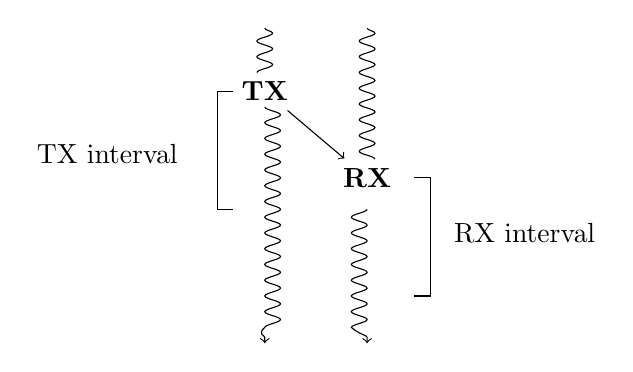
\begin{tikzpicture}
      \draw[->,decorate,decoration={snake,segment length=2mm, amplitude=1mm}]
        (0mm,0mm) -- (0,-5mm)
        (0mm,-8mm) node (TX) {\textbf{TX}} (0,-10mm) --
        (0mm,-40mm);
      \draw (-4mm,-8mm) -- (-6mm,-8mm) -- (-6mm,-23mm) -- (-4mm,-23mm);
      \draw (-20mm,-16mm) node {TX interval};

      \draw[->,decorate,decoration={snake,segment length=2mm, amplitude=1mm}]
        (13mm,0mm) -- (13mm,-16mm)
        (13mm,-19mm) node (RX) {\textbf{RX}} (13mm,-23mm) --
        (13mm,-40mm);
      \draw (19mm,-19mm) -- (21mm,-19mm) -- (21mm,-34mm) -- (19mm,-34mm);
      \draw (33mm,-26mm) node {RX interval};
      \draw[->] (TX) -- (RX);
    \end{tikzpicture}
    \label{fig:enforce:message_windows:tx_first}
  }
  \subfigure[][Intervals overlap; message is sent]{
    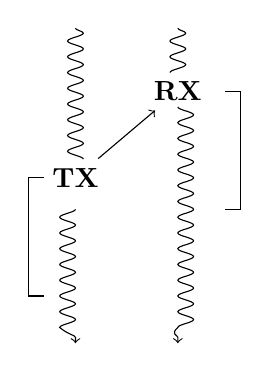
\begin{tikzpicture}
      \draw[->,decorate,decoration={snake,segment length=2mm, amplitude=1mm}]
        (0mm,0mm) -- (0,-16mm)
        (0mm,-19mm) node (TX) {\textbf{TX}} (0,-23mm) --
        (0mm,-40mm);
      \draw (-4mm,-19mm) -- (-6mm,-19mm) -- (-6mm,-34mm) -- (-4mm,-34mm);

      \draw[->,decorate,decoration={snake,segment length=2mm, amplitude=1mm}]
        (13mm,0mm) -- (13mm,-5mm)
        (13mm,-8mm) node (RX) {\textbf{RX}} (13mm,-10mm) --
        (13mm,-40mm);
      \draw (19mm,-8mm) -- (21mm,-8mm) -- (21mm,-23mm) -- (19mm,-23mm);
      \draw[->] (TX) -- (RX);
    \end{tikzpicture}
    \label{fig:enforce:message_windows:rx_first}
  }
  {\hfill}
  \subfigure[][Intervals do not overlap; no message can be sent.]{
    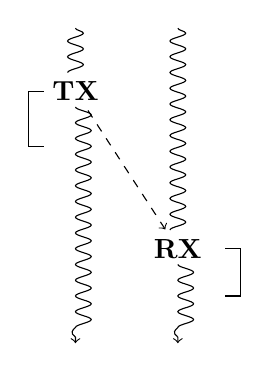
\begin{tikzpicture}
      \draw[->,decorate,decoration={snake,segment length=2mm, amplitude=1mm}]
        (0mm,0mm) -- (0,-5mm)
        (0mm,-8mm) node (TX) {\textbf{TX}} (0,-10mm) --
        (0mm,-40mm);
      \draw (-4mm,-8mm) -- (-6mm,-8mm) -- (-6mm,-15mm) -- (-4mm,-15mm);

      \draw[->,decorate,decoration={snake,segment length=2mm, amplitude=1mm}]
        (13mm,0mm) -- (13mm,-25mm)
        (13mm,-28mm) node (RX) {\textbf{RX}} (13mm,-30mm) --
        (13mm,-40mm);
      \draw (19mm,-28mm) -- (21mm,-28mm) -- (21mm,-34mm) -- (19mm,-34mm);

      \draw[->,dashed] (TX) -- (RX);
    \end{tikzpicture}
    \label{fig:enforce:message_windows:failed}
  }
  \caption{Overlapping TX and RX intervals allow the message to be
    sent, regardless of which operation is ordered first.  If the
    intervals do not overlap then no message can be sent. \todo{Fix diagram}}
  \label{fig:enforce:message_windows}
\end{figure}

Suppose, for instance, that the interval were set at 20ms.  A
\textbf{TX} operation were to occur at time 512ms would then be able
to communicate with an \textbf{RX} operation at 520ms.  This would
involve delaying the transmitting thread by 8ms so that the two
operations occur at the same time.  Similarly, the \textbf{TX}
operation could communicate with an \textbf{RX} at 498ms by delaying
the receiving thread by 14ms.  It would not, however, be possible for
the \textbf{TX} operation to communicate with \textbf{RX} operations
at 490ms or 540ms, because those fall outside of the interval.

There are two complications in implementing this behaviour.  First, it
is difficult for a \textbf{TX} operation to look ahead through the
execution to determine how long it should wait for the \textbf{RX}
operation to arrive, or vice versa.  Second, it might be that several
possible partner operations happen during the interval, and the LLI
must decide which to bind to.  In practice, it is not possible to
completely solve these problems and get precisely the desired
behaviour, but it is possible to approximate it reasonably accurately.
{\Implementation} uses the following algorithm to implement the peer
selection part of the \textbf{TX} algorithm; the \textbf{RX} algorithm
is symmetric:

\begin{itemize}
\item[1] Iterate over the global \texttt{rx\_thread} table.  All of
  the entries in this table will be LLIs which are currently at the
  \textbf{RX} state.  Compare the message which this LLI wants to
  transmit to the message which the other LLI wants to receive.  If
  they match, and if any side-condition on the message passes, the
  local LLI completes both message operations.  This means that it
  duplicates both LLIs, copies the necessary state between the two new
  LLIs, advances them past the message operation, and adds them back
  to the appropriate HLIs.
\item[2] Register the current LLI in the global \texttt{tx\_thread}
  table.
\item[3] Sleep for the interval.
\item[4] De-register the current LLI from the \texttt{tx\_thread}
  table.
\item[5] The current LLI now corresponds to the situation where no
  other threads arrived during the interval, and so it has failed and
  should exit.
\end{itemize}

The intent is that when a new \textbf{TX} operation starts, it first
looks for any existing \textbf{RX} operations which are waiting for
it, corresponding to
Figure~\ref{fig:enforce:message_windows:rx_first}.  If it finds any,
it completes both operations, creating new LLIs on both the receive
and transmit side to store its results.  It then goes to sleep waiting
for any further \textbf{RX} operations, corresponding to
Figure~\ref{fig:enforce:message_windows:tx_first}.  If any \textbf{RX}
operations arrive during this window then they will complete both the
\textbf{TX} and \textbf{RX} operations, and so when the sleep
completes the current LLI has no more to do and should exit,
corresponding to
Figure~\ref{fig:enforce:message_windows:failed}\footnote{{\Implementation}
  actually includes an optimisation to avoid creating and destroying
  LLIs unnecessarily in the common case where precisely one peer
  operation is available, but this does not fundamentally alter the
  algorithm and is not shown here.  Likewise, this discussion omits
  the enforcer-internal synchronisation necessary to implement this
  algorithm in a race-free way, to avoid unnecessarily complicating
  the presentation.}.

This algorithm solves the problem of not knowing how long to wait by
always waiting for the maximum possible time, and the problem of not
knowing which of many possible peers to synchronise with by simply
synchronising with all of them.  That is similar to but not quite
identical to the desired behaviour.  In particular, in the desired
semantics, when a message operation is destined to fail, it should not
wait at all, whereas here failing operations wait for the maximum
possible time.  In other words, the non-deterministic part of the
desired behaviour is correctly implemented, but the non-causal part is
not.  In practice, the only effect of this is to sometimes cause poor
performance, by introducing completely redundant delays.  If it were
necessary, the correct behaviour could be achieved using a
deterministic replay system\needCite{} and techniques similar to a
time-travelling debugger\needCite{}, but doing so would almost
certainly not fix the performance problems.  I have not investigate
this at all.

Observant readers will have noticed that this algorithm is itself
unimplementable.  It is common for a single HLI, and hence a single
concrete program thread to run multiple LLIs, and it is not possible
to delay one LLI in a thread without delay all of the others.  What,
then, should the enforcer do if the different LLIs need to perform
different message operations?  There are several interesting cases:

\begin{itemize}
\item Multiple LLIs need to perform unbound message operations at the
  same time.  In that case, they will all need to delay, and so the
  enforcer can just run steps one and two of the algorithm for each
  LLI, then perform a single delay step three, and then run steps four
  and five for each LLI.
\item One LLI $l_1$ needs to perform an unbound message operation
  while another $l_2$ has already completed a message operation.
  $l_2$ will have a bound thread, $l_3$.  In order to delay $l_1$ we
  must also delay $l_2$, and there is a risk that it will then miss
  its next deadline for communicating with $l_3$, causing both $l_2$
  and $l_3$ to fail.

  The problem here is type of timeout used by $l_3$.  In the simple
  low-level interpreter described in Section~\ref{sect:enforce:llis},
  $l_3$ considers $l_2$ to have failed to reach its message operation
  if $l_3$ has to wait more than fixed time for $l_2$ to arrive.  An
  equally valid definition would be to say that $l_2$ has some fixed
  amount of time to move from its $n$th message operation to its
  $(n+1)$th.  In that case, it is easy\editorial{This is a lie.  It
    was actually a complete pain in the arse, but I don't want to go
    into the details, so I'm going to wave my hands a bit and pretend
    it was easy.} to arrange that time spent waiting because of $l_1$
  does not count towards $l_2$'s deadline, hence allowing $l_3$ to
  eventually complete its message operation.
\item One LLI $l_1$ needs to perform an unbound message operation,
  while another LLI $l_2$ has yet to reach its first message
  operation.  In this case, an ideal enforcer would delay $l_1$ but
  not $l_2$ but, as already discussed, this is impossible in a real
  system.  Fortunately, delaying $l_2$ is unlikely to cause
  significant problems here, as it does not yet have a bound LLI, and
  there are therefore no enforcer-level constructs waiting for it in
  any other program threads.
\end{itemize}
    
All\editorial{All I've thought of, anyway} other cases can be reduced
to some combination of these.

The interactions with the \textbf{Succ} phase present a further
complication.  The \textbf{Succ} thread will sometimes need to
duplicate an LLI in order to handle ambiguities in the CFG.  If done
na\"ively, this might lead to a single LLI being bound to multiple
other LLIs.  For instance, if $l_1$ and $l_2$ are bound together and
$l_1$ is duplicated to $l_1'$, the obvious implementation would bind
$l_2$ to both $l_1$ and $l_1'$, which would then cause problems the
next time $l_2$ attempts a message operation.  At the same time,
it is clearly incorrect for $l_1'$ to be created unbound.
The solution is simple: duplicate $l_2$ at the same time as $l_1$
is duplicated, so that $l_1$ remains bound to $l_2$ and $l_1'$ is
bound to $l_2'$.

\subsubsection{Selecting the size of the timeout}
\label{sect:using:timeout_balancing}

Up to now, the discussion has assumed that all timeouts are the same,
fixed, size.  This is not always the best possible strategy.  In
particular, it is not always necessary or useful to delay both the
transmit and receive halves of a message operation.  I now show that
one of these delays can usually be omitted, and give a brief
discussion of how to decide which to omit.

Unbound timeouts are generally far more important than bound ones, in
terms of both their effects on the time taken to reproduce the bug and
their effects on the program's performance while running under the
enforcer, as the construction of the plan, and in particular the
selection of side-conditions, ensures that bound messages will only
happen when the target bug has a very high chance of reproducing.
Assume, then, that only unbound delays matter.  Assume further that
the enforcer is only trying to enforce one happens-before graph, that
there are only two threads in the program, and that the delay is small
enough that it does not meaningfully affect the program's behaviour.
There will then be only two message operations to consider, one
\textbf{TX} and one \textbf{RX}, and they will both occur with some
fixed frequency.  Call these frequencies $f_{\mathbf{TX}}$ and
$f_{\mathbf{RX}}$ and call the delays imposed by each operation
$D_{\mathbf{TX}}$ and $D_{\mathbf{RX}}$.

We can then easily estimate the performance cost of the enforcer.  The
fraction of program time spent in those delays is then
$f_{\mathbf{TX}}.D_{\mathbf{TX}} + f_{\mathbf{RX}}.D_{\mathbf{RX}}$,
and that is a reasonable proxy for the overhead $\omega$.

Next, estimate the expected time before the bug is reproduced.  One
way for the bug to reproduce is if the \textbf{TX} might occurs within
$D_{\mathbf{RX}}$ after a \textbf{RX} operation.  In effect, each
\textbf{RX} operation defines a window of size $D_{\mathbf{RX}}$ in
the program's timeline and the bug reproduces if a \textbf{TX} effect
lands in that window.  These windows will cover a fraction
$f_{\mathbf{RX}}.D_{\mathbf{RX}}$ of the timeline, and so, assuming
\textbf{TX}s occur randomly, each will have a probability of
$f_{\mathbf{RX}}.D_{\mathbf{RX}}$ of triggering the bug, giving a bug
reproduction rate of
$f_{\mathbf{TX}}.f_{\mathbf{RX}}.D_{\mathbf{RX}}$.  Symmetrically, the
bug might be reproduced if a \textbf{RX} operation occurs
$D_{\mathbf{TX}}$ after a \textbf{TX} one, giving a reproduction rate
of $f_{\mathbf{TX}}.f_{\mathbf{RX}}.D_{\mathbf{TX}}$.  These are the
only ways in which the bug can reproduce, and so the total
reproduction rate $\rho$ is
$f_{\mathbf{TX}}.f_{\mathbf{RX}}.(D_{\mathbf{RX}} + D_{\mathbf{TX}})$.

The task is now to choose $D$ so as to maximise the reproduction
rate whilst minimising the overhead.  Some simple algebra is
sufficient to show that

\begin{displaymath}
\rho = {\omega}.f_{\mathbf{RX}} + f_{\mathbf{RX}}.D_{\mathbf{RX}}(f_{\mathbf{TX}} - f_{\mathbf{RX}})
\end{displaymath}

In other words, if $f_{\mathbf{TX}} > f_{\mathbf{RX}}$ then the
reproduction rate for a given level of overhead is maximised by
setting $D_{\mathbf{RX}}$ as large as possible and $D_{\mathbf{TX}}$
to zero, and conversely when $f_{\mathbf{TX}} < f_{\mathbf{RX}}$.
{\Implementation} therefore keeps a counter of how many times the send
and receive sides of each message operation are attempted; if the send
operation has been attempted more times than the receive one then the
send operation delay is set to zero, and otherwise the receive delay
is set to zero.  The other delay is set to some user-configured
constant.

\subsection{Run-time considerations}

Evaluating side conditions is not always completely trivial, even once
all of the inputs are available.  In particular, $LD(addr)$
expressions require a moderate amount of care.  These are defined to
return the contents of memory at a particular address.  The problem is
that the address might turn out to be a bad pointer, and it is
important for the enforcer not to cause the program to crash in that
case.  {\Implementation} solves this problem by simply catching page
faults generated while evaluating side conditions.  If any such faults
occur then the relevant LLI is considered to have failed.  This is not
always ideal from the point of view of reproducing the bug, but avoids
spuriously crashing the program under test.

\todo{Why do we sometimes end up dereferencing pointers which the
  program never does? Answer: because the placement stuff sometimes
  ends up pulling validation over program control flow, which makes it
  easier to implement and easier to fast-out of the enforcer, but
  risks introducing these bad dereferences.}

Another approximation is that $LD$ expressions are defined to return
the ``initial'' contents of memory, but in {\implementation} they
instead return the contents of memory as soon as the address to be
loaded becomes evaluatable.  This might be different if the address
depends on some piece of program state which only becomes available to
the interpreter some time after the plan has started, as some other
program thread might modify memory in the meantime.  This is not
usually a serious issue, as the interpreter usually becomes able to
evaluate the address before the program itself is, and so can capture
the contents of a memory location at the first point where the code
being investigated might possibly have observed it.  That is usually
sufficient to evaluate the side-condition\editorial{Not sure how clear
  that really is.}.

\section{Gaining control of a running program}
\label{sect:enforce:gain_control}

Section~\ref{sect:reproducing_bugs} describes how to make bugs more
likely to reproduce, assuming that it can gain control of the program
at any point.  This section describes one possible way of doing so.
{\Implementation} does so by modifying the original program to contain
branches into the plan interpreter where necessary.  This has very low
runtime overhead and avoids excessively permuting the program's state,
but has one critical disadvantage: the instruction at which
{\implementation} needs to gain control might be smaller than a branch
instruction, and so inserting the branch might cause additional
instructions in the program binary to be corrupted.  {\Implementation}
must then ensure that the program never attempts to execute one of
these corrupted instructions.  For performance reasons, we would also
like to minimise the number of instructions which must be run in the
interpreter.

This is most easily understood as a kind of search problem.  The
algorithm starts in a state in which the original program is not
modified at all, but with a list of instructions at which it must gain
control; it must then find a path to a state in which it is guaranteed
to gain control at all necessary points and the program is guaranteed
never to branch to a corrupted instruction.  More explicitly, these
states consist of three sets:

\begin{itemize}
\item $\mathit{Patch}$ --- instructions at which we have decided to place a
  branch instruction.
\item $\mathit{Cont}$ --- instructions which might not themselves be
  patched, but which must be processed in the interpreter.  The
  program will not branch to the interpreter when it encounters one of
  these instructions, but if the interpreter has already started when
  one needs to be run then the interpreter will continue, even if the
  enforcement plan itself does not require that.
\item $\mathit{MustInterpret}$ --- instructions where the enforcement
  plan requires us to gain control, but where the patches described in
  this state would be insufficient to do so.
\end{itemize}

The search process then generates additional states according to two
rules:

\begin{itemize}
\item
  \textbf{PatchDirect} An instruction is removed from
  $\mathit{MustInterpret}$ and added to $\mathit{Patch}$.  The
  analysis then examines the instructions which would be corrupted by
  that new entry point to determine whether there are any potential
  branches to them and, if so, adds those branches to
  $\mathit{MustInterpret}$.  The corrupted instructions are themselves
  added to $\mathit{Cont}$.

  This rule is only valid when the existing $\mathit{Patch}$ set does
  not itself contain any patch operations which would overlap with the
  new patch point, as these branch instructions would otherwise
  corrupt each other and lead to an unrealisable solution.
\item
  \textbf{Prefix} As with \textbf{PatchDirect}, an instruction is
  removed from $\mathit{MustInterpret}$, but in this case it is added
  to $\mathit{Cont}$ and any instruction which might branch to it
  added to $\mathit{MustInterpret}$.  The idea here is that if we can
  ensure that all instructions which execute immediately prior to an
  instruction $i$ are executed in the interpreter and if the
  interpreter continues interpreting when it sees a branch to $i$ then
  that is sufficient to ensure that $i$ is also run in the
  interpreter.
\end{itemize}

Any state with an empty $\mathit{MustInterpret}$ set then represents a
valid solution to the patching problem.  The number of instructions in
$\mathit{Cont}$ is a rough proxy for the number of additional
instructions which will have to be interpreted due to the corrupted
instructions problem, and hence for the overheads of the patching
process, and so the search process aims to minimise the
$\mathit{Cont}$ set.  Usefully, both rules increase the size of
$\mathit{Cont}$ and so a simple exploration strategy which always
selects the state in the queue with the smallest $\mathit{Cont}$ set,
applies both rules to that state, and places the two new states in the
queue is guaranteed to always find the minimal result, and this is the
strategy adopted by {\implementation}.

One complication here is that the algorithm needs to be able to find
the predecessors of an instruction.  In the fully general case this is
an impossible thing to determine for an arbitrary binary.
{\Technique} makes two key assumptions in order to solve it:

\begin{itemize}
\item
  Functions are only ever entered at their entry point, as determined
  by the analysis described in Section~\ref{sect:function_head}.  In
  particular, any branches from dynamically generated or library code
  back into the main program must branch to a function head.
\item
  For any dynamic branch within a function, the dynamic analysis
  observes all possible targets of that branch.
\end{itemize}

Given those assumptions, the static analyses already discussed can
determine all of the branches to any instruction in the program except
for a function head, and can detect whether an instruction is a
function head.  {\Technique} then simply disables any rule which
requires it to calculate the predecessors of a function head.

This can sometimes lead to the patch problem being unsolvable if the
entire function is smaller than a single branch instruction, as in
that case it is possible that neither rule might be enabled at the
function head.  In that case, {\implementation} simply gives up and
reports an error.  This is rarely a problem in practice, as very few
functions are that small without very aggressive compiler
optimisations, and most compilers, including gcc and LLVM\needCite{},
will at high optimisation levels pad functions to a multiple of 16
bytes for performance reasons.

The assumption that the dynamic analysis is complete is more of a
problem.  This can sometimes lead to the program executing one of the
corrupted instructions if its behaviour deviates significantly from
that observed during dynamic analysis.  That is just about tolerable
in a tool such as {\technique}'s crash enforcers, which are only
intended as a debugging aid for knowledgeable programmers, but is more
of a concern when {\technique} is being used to fix bugs. \todo{I'm
  going to need to say something clever here.}

This problem was also tackled by the AutoPaG project, and the solution
they developed is similar. \todo{Similar but not the same.  They use a
  dominator-based scheme, and hence avoid needing the global branch
  information but can end up with much larger patches and a higher
  risk of deadlocks/starvation problems.  The original version of
  {\technique} used basically the same algorithm (although I did it
  first); should probably explain why I had to switch.}

An alternative approach would be to take control of the program using
debug breakpoints rather than jump instructions.  These are either a
single byte (for the \verb|int3| instruction) or no bytes at all (for
debug registers), and so avoid the instruction clobbering problem.
This would work, but would have a couple of important disadvantages:

\begin{itemize}
\item
  Debug breakpoints are far slower than branches.  This might be
  important if the critical section\editorial{?} is to be inserted on
  a particularly hot code path and has a side-condition which usually
  fails.
\item
  Using debug breakpoints in this way would interfere with any other
  debugger which the developer might want to use.  With a branch-style
  patch, standard debuggers work without modification for any part of
  the program which has not been patched, whereas a breakpoint-style
  patch requires extensive coordination between the debugger and the
  patch mechanism for either to work at all.
\item
  Breakpoint registers are of strictly limited number on most
  architectures (four, on x86).  This means that they can never
  provide a complete solution by themselves.
\item
  On most UNIX-type operating systems, including Linux and FreeBSD,
  catching debug breakpoints requires modifying the program's signal
  handling configuration, which requires some level of coordination
  with the program to be modified.  It would be possible to use an
  alternative API, but this would require kernel modifications,
  complicating the use of the generated patches.
\end{itemize}

{\Implementation} therefore generates exclusively branch-style patches.

\todo{I did implement a breakpoint-based scheme, so it might be
  interesting to actually include some numbers on their relative
  effectiveness.}

\todo{Placing patch points is actually the most computationally
  expensive step of building the enforcer, once you've got the VC.  I
  might need to do some implementation work to make that a bit less
  crazy.}

Of course, a patch strategy which ensures that the interpreter gains
control at appropriate instructions is not quite the same as one which
ensures that the interpreter gains control at appropriate CFG nodes,
because {\technique} CFG nodes are identified by stack context in
addition to their raw instruction pointer.  The interpreter must
therefore be able to check this call stack.  

The interpreter has access to all of the process registers and the
stack when it gains control.  The challenge here is to locate the
return addresses on the stack, without access to either debug symbols
or a frame pointer, so that the function calling context can be
properly checked.  {\Technique} uses a static analysis, performed when
generating the crash enforcement plan, to solve this problem.  The
static analyses already described are sufficient to determine the
entry point of the function containing a given instruction pointer,
and so it is easy to perform a simple abstract interpretation forwards
from that point to the given instruction pointer and hence find the
number of bytes which the function will push onto the stack on the
way\footnote{This is generally fixed for all possible paths, due to
  the way in which most compilers are implemented.}.  The first entry
in the call stack is trivially true because of the way the jumps are
patched in.  The second one is the return address of the current
function, which can be found using that offset.  The third one is the
return address of the calling function, and the offset there is just
the previous offset plus the offset in the calling function.  In this
way all necessary offsets can be found and the entry-point stack
checked completely.  \todo{Rewrite para}

\section{Fixing bugs using global locks}
\label{sect:fix_global_lock}

In addition to finding bugs, {\technique} can also be used to fix
them.  The basic approach here is to binary patch the program to
introduce a new global lock covering the program's relevant
instructions, preventing them from executing in parallel and hence
preventing the bug from occurring (assuming that the relevant
instructions have been correctly identified).  The relevant
instructions are duplicated into a binary patch, unrolling loops and
tracing across function boundaries in a way which reflects the
function inlining and loop unrolling performed during the initial CFG
generation phase, and the duplicates modified to acquire and release
the lock at appropriate points.  The original program is then patched
to branch to the duplicates when necessary.

\subsection{Identifying the instructions which must be protected}

The first step in producing such a fix is correctly identifying the
instructions which must be included in the critical sections.  These
will be roughly a subset of the instructions involved in the
control-flow graphs associated with \StateMachines; a ``subset''
because some instructions in the CFG do not need to be protected, and
``roughly'' because some instructions not in the CFG will also be
included in the critical section.

As an example of the former, consider a program like this:

\begin{verbatim}
crashing_thread() {
    ptr = complicated_local_calculation();
    dptr = *ptr;
    if (dptr != NULL) {
       dptr = *ptr;
       *dptr = 5;
    }
}
interfering_thread() {
    ptr = complicated_local_calculation();
    *ptr = NULL;
}
\end{verbatim}

Here, the crashing thread computes some pointer using entirely local
operations, loads from it once and then, if the result is
non-\texttt{NULL}, loads from it again and uses the resulting pointer.
Meanwhile, the interfering thread sets a potentially coincident memory
location to \texttt{NULL}.  The crashing thread clearly has a
potential time-of-check, time-of-use race bug.  The {\StateMachines}
generated by {\technique} will include the buggy code itself but might
also include part or all of \texttt|complicated\_local\_calculation()|
and a side-condition which requires the two pointers to match up.
This extra information is useful when analysing the bug
(Section~\ref{sect:using:check_realness}) or when attempting to reproduce it
(Section~\ref{sect:reproducing_bugs}), but cannot be used by this kind
of instruction-level fix\footnote{But see future work for a possible
  alternative scheme which would make use of it.}, so including it in
the fix is unhelpful and would tend to lead to unnecessarily large
critical sections.  The fix generating process must therefore select a
useful subset of the instructions in the control-flow graph.

The approach taken here is simple:

\begin{itemize}
\item
  Extract all of the happens-before edges from the bug summary's
  verification condition.  These entirely capture the
  instruction-interleaving parts of the bug to be fixed, and, since
  instruction-interleaving is the only thing which can be influenced
  by inserting locks, the resulting set of edges contains all of the
  useful information in the condition.
\item
  Identify all of the CFG nodes which are mentioned in one of those
  happens-before edges.
\item
  Trim the CFG such that every path starts and ends in one of those
  mentioned nodes.  All such paths will be included in a critical
  section, and so no such paths will be permitted to execute in
  parallel.
\end{itemize}

In this way the CFG is restricted to just those instructions which are
involved in the interleaving which is to be prevented.

Note that this is not guaranteed to produce an optimal selection of
critical sections, in the sense that sections can sometimes be larger
than is strictly necessary.  Consider, for example, a program with the
same crashing thread as the previous example but an interfering thread
in which the pointer is assigned to twice:

\begin{verbatim}
interfering_thread() {
    ptr = complicated_local_calculation();
    *ptr = NULL;
    *ptr = NULL;
}
\end{verbatim}
    
There are now two obvious ways of protecting this program:

\begin{itemize}
\item
  Place both loads in the crashing thread in a single critical section and
  both stores in the interfering thread in another one.
\item
  Place both loads in the crashing side in a single critical section,
  but give each store in the interfering thread its own critical
  section.  In other words, drop and re-acquire the lock in between
  the two stores.
\end{itemize}

Both approaches correctly eliminate the bug, but they will have
different performance characteristics.  In particular, dropping and
re-acquiring the lock reduces the size of the critical section, which
might improve concurrency and reduce starvation, but imposes higher
overheads due to the greater number of lock operations.  In principle
the verification condition contains enough information to determine
whether dropping the lock is safe, but {\technique} does not make use
of this information, and always uses the former strategy.

\subsection{The interpreter}

\todo{Rewrite paragraph.} The input to this phase of {\technique} is a
fix plan, which consists of a set of CFG fragments such that the bug
will be fixed if {\technique} can arrange that two fragments never run
in parallel with each other.  The output of the phase is a modified
version of the program which ensures just that.  To explain how this
works, I first show how to modify a hypothetical machine-code
interpreter to enforce the fix and then show how to convert such an
interpreter into a compiler.  The resulting compiler generates a
modified version of the program which enforces the plan with very low
run-time overhead.

The goal of the interpreter is to emulate the original program's
machine code in a way which ensures that if one thread enters a
protected CFG then no other thread is able to enter a protected CFG
until the original thread has left the protected CFG.  There are two
important complications here:
                                                                                                                                                                             
\begin{itemize}
\item The CFG to be protected is a fragment of the unrolled CFG used
  when building state machines, rather than the program's actual CFG.
  This means that one program instruction might potentially be
  represented by several CFG nodes, and given a simple instruction
  pointer it is not always possible to determine where in the CFG a
  thread is currently executing.

\item CFG fragments might sometimes overlap, and the interpreter must
  ensure that the program does not allow concurrent execution until
  every relevant fragment has finished.  At the same time, it must
  also ensure that the program cannot acquire the same lock multiple
  times, to avoid the risk of self-deadlocks.
\end{itemize}

Solving these issues is relatively simple.  The interpreter simply
keeps track of the set of CFG nodes which each thread might
potentially be executing and arranges to acquire the lock whenever
this set goes from empty to non-empty and to release it whenever it
goes from non-empty to empty.  This is analogous to the way in which
enforcers handle ambiguity in the \textbf{Succ} phase (see
Section~\ref{sect:enforce:succ}).

I now give a little more detail of the interpreter.  At this stage,
assume that the entire program is run in the interpreter; later
sections show how to reduce the amount of the program which must be
interpreted and eventually eliminate the interpreter completely.

When running, the interpreter cycles repeatedly through these phases:

\begin{itemize}
\item \textbf{CheckForEntry} The interpreter checks whether the
  current instruction is the entry point of any other CFG fragments.
  If it is, the relevant CFG node is added to the current set of
  active CFG nodes.  Note that this potentially involves checking the
  thread's function call stack in addition to its current instruction
  pointer.

\item \textbf{Lock} The interpreter now acquires the patch lock, with
  a timeout, provided that it does not currently own it and the set of
  active CFG nodes is non-empty.  If the lock times out then the
  interpreter gives up on trying to protect the program; this
  introduces a risk of the bug reproduces, but is necessary to avoid a
  potential deadlock with the program's own synchronisation strategy.

\item \textbf{Emul} The interpreter runs the instruction from the
  original program, performing any necessary memory accesses or
  register updates.  This is essentially the same as the phase of the
  same name in the enforcer's LLI loop (see
  Section~\ref{sect:enforce:llis}).

\item \textbf{Succ} The \textbf{Emul} phase will have computed the
  instruction pointer of the next instruction to be executed.  This
  can then be compared to the set of currently active CFG nodes and to
  the CFG fragment which is to be protected to calculate a new set of
  active CFG nodes.  Again, this is analogous to the phase of the same
  name in the enforcer's LLI loop.

\item \textbf{Unlock} Finally, the interpreter can now consider
  releasing the patch lock.  It does so if it currently holds the lock
  and the set of active CFG nodes has become empty.  The instruction
  cycle then restarts at \textbf{CheckForEntry}.
\end{itemize}

This scheme ensures that the lock is always held when instructions
from the original program execute if there is any possibility that the
thread is currently executing one of the CFG fragments.  At the same
time, it correctly ensures that the lock is never double-acquired or
double-released.  It therefore correctly implements the desired fix,
but at the expense of potentially very high overhead due to running
the entire program in an interpreter.

\subsection{Running unprotected code without an interpreter}

The most important source of undesired overhead in this scheme is that
the entire program must run in the interpreter, even the parts which
are not being protected by the fix.  The common case is that the fix
protects a very small fraction of the total instructions in the
program, and so this is extremely inefficient.  Fortunately, it is
also reasonably easy to fix.  Section~\ref{sect:enforce:gain_control}
has already described a scheme for binary patching a program to gain
control at a defined set of instructions, and this can be used
unmodified here.  The interpreter starts in the \textbf{CheckForEntry}
phase with an empty set of active CFG nodes and not holding the lock.
It is then only necessary to introduce an additional \textbf{Return}
phase in between \textbf{CheckForEntry} and \textbf{Lock} which
transfers control from the interpreter back to the original program if
the active CFG node set has become empty.

One slight complication here is that the patch strategy might need to
modify the program in places other than the instructions at which it
must gain control, and so might have to extend the set of instructions
which are to be interpreted; in the terminology of
Section~\ref{sect:enforce:gain_control}, it might have a non-empty
$\mathit{Cont}$ set.  If so, the implementation of the \textbf{Return}
phase must be careful not to return to an instruction in the
$\mathit{Cont}$ set and must instead continue interpreting.  This is
straightforward to arrange.

One possibly surprising property of this design is that, even with
this refinement, the interpreter can still sometimes run while not
holding the lock if the program is executing $\mathit{Cont}$
instructions.  An alternative approach would be to simply acquire the
lock when the interpreter starts running and release it when the
interpreter exits.  This would be a valid approach, and would perhaps
result in a very slightly simpler implementation, but at the expense
of enlarging the size of the critical sections slightly.  In practice
this decision very rarely makes any meaningful difference.  The main
exception occurs if protecting the $\mathit{Cont}$ set would cause the
critical section to span an entire loop rather than just a single
iteration of it, which could potentially aggravate the liveness and
fairness issues which are inherent to any lock-based scheme.

\subsection{Recompiling the protected code with additional protection}

This scheme allows the program to run at native speed when executing
code which does not have to be protected, but still requires it to be
interpreted when in the critical sections.  This can sometimes be an
issue if the bug to be fixed is a rare one in a very hot path.
{\Implementation} therefore includes a mechanism to recompile the
protected code back into machine code with the necessary additional
synchronisation added.  One productive way of thinking of this is to
say that the interpreter has been supercompiled or partially evaluated
so as to fix both the fix plan and the original program's machine
code, leaving only the original program's external inputs unspecified.

The main complication here is that the compiled fix has no good way of
storing its state: registers and the stack are unavailable, as they
are used by the program to be protected; main memory does not work,
because most of the state needs to be thread-local; and anything based
on system calls is undesirable because the state needs to be accessed
so frequently, sometimes multiple times per instruction.  The approach
taken by {\implementation} is to, in effect, encode the per-thread
state into the program's instruction pointer, creating a duplicate of
each program instruction for each interpreter state which that program
instruction might execute in.  This is practical because the number of
interpreter states per program instruction is usually very small,
often just one, and so the number of duplicates is manageable.

One major advantage of this instruction duplication approach is that
the supercompiler knows, when emitting an instruction, precisely what
state the interpreter is in, and so a quite na\"ive implementation can
still generate reasonably efficient machine code for the interpreter
operations.  Further, most instructions in the original program can be
copied across without modification, and so most compiler optimisations
applied to the original program continue to be effective in the
patched version.

One way of thinking about this is to say that the program's
instruction pointer is replaced with a more complicated structure
containing both the original pointer and the state of the interpreter.
The state of the interpreter is itself a three-tuple containing the
current set of active CFG nodes, a flag saying whether the lock is
currently held, and the instruction cycle phase.  The interpreter
described above shows how the original program's CFG can be combined
with the fix plan to give a new CFG expressed in terms of these
extended instruction pointers, and the compiler then lowers this
extended CFG back into ordinary machine code.  The lowering process
itself is easiest to think about as a kind of partial evaluation:

\begin{itemize}
\item \textbf{Lock} phases partially evaluate to either the machine
  code for a lock operation (if the lock is not currently held and the
  set of active CFG nodes is non-empty) or a no-op (otherwise).

\item \textbf{Unlock} phases likewise evaluate to either the machine
  code for an unlock operation or a no-op.
\item \textbf{Return} partially evaluates to either a no-op (usually)
  or a branch back to the original program (if the set of active CFG
  nodes is empty and the current instruction pointer is not in
  $\mathit{Cont}$).

\item \textbf{CheckForEntry} evaluates to a context validation tree,
  discussed below.

\item \textbf{Issue} will usually partially evaluate to the program's
  original instruction, which can be emitted unchanged into the final
  patch.  The two exceptions are instruction pointer-relative
  addressing modes, which must be re-encoded to still refer to the
  same data after moving the instruction, and control flow transfer
  instructions, which are discussed below.
\end{itemize}

The result of partially evaluating the nodes in the extended CFG is a
set of fragments of machine code which can then be stitched back
together to form the core of the new patch.

\subsection{Context validation trees}

The \textbf{CheckForEntry} phase is responsible for checking whether
the program thread has just entered the start of a new protected CFG
fragment and extending the set of active CFG nodes if appropriate.
This obviously involves checking whether the current instruction
pointer matches with any of those entry-point CFG nodes, and that part
of the check is very easy.  More difficult is checking the
instruction's calling context.  {\Technique} can handle some
cross-function bug behaviour, which can sometimes lead to instructions
being protected in different ways depending on which function called
them.  This calling context is expressed as a list of return addresses
$ra_1$, $ra_2$, $\ldots$, $ra_n$, where $ra_1$ is the return address
of the current function, $ra_2$ the return address of the calling
function, $ra_3$ the return address of that function's caller, and so
forth.  The \textbf{CheckForEntry} phase must check that the context
matches in addition to checking the raw instruction pointer.  There
are a number of important complications in doing so:

\begin{itemize}
\item The program to be modified might lack frame pointers and debug
  information, and this can make it non-trivial to locate the return
  address on the stack.  This has already been discussed on pages 24
  and 25, in the context of extracting call stacks from core dumps,
  and essentially the same algorithm works here as well.  This allows
  SLI to determine, for each return address in a call context, where
  on the stack that return address is expected to be found, as an
  offset from the current stack pointer.
\item It is not necessarily safe to access every stack location
  involved in a calling context.  In particular, if a particularly
  deep context is checked while the program is actually in a
  particularly shallow one then the addresses at the top of the deep
  context might be beyond the limit of the processor stack, and so
  accessing them would risk causing a segmentation violation \todo{(or
    whatever the platform equivalent is)}.  This problem can be
  avoided if \textbf{CheckForEntry} is careful to always check call
  contexts starting at the bottom (i.e. the return address location
  nearest to the current stack pointer).  This is safe because if
  $ra_i$ matches the desired value then that ensures that all of the
  functions up to $i$ in the call chain, which means that $ra_{i+1}$
  will be in the expected place on the stack and can be accessed
  without fear of a segmentation fault\footnote{The only exception
    here is if there is some function on the stack which cannot return
    without immediately underflowing the stack.  The only common
    functions of that form, at least on Linux, are
    \texttt{\_\_libc\_start\_main} and \texttt{start\_thread}, both of
    which are in libc, and SLI will not attempt to fix bugs in system
    libraries.}

  \todo{This is a really obvious point which I'm explaining really
    badly.}
\item It might sometimes be that one calling context is a subset of
  another.  For example, it might be that instruction A should always
  start CFG node X, and should in addition start CFG node Y if its
  return address is B.  \textbf{CheckForEntry} must correctly handle
  this case.
\item And, of course, we would like the context checking to itself
  have minimal overhead.  In particular, if the currently-active CFG
  node set is empty then that will constrain the call contexts which
  the thread might currently occupy, and it would be useful to avoid
  redundantly testing stack locations whose values are already fixed
  by these constraints.
\end{itemize}

The algorithm used by the interpreter is then reasonably simple:                                                                                                             

\begin{enumerate}
\item Collect up all of the possible entry point CFG nodes for this
  instruction, along with their call contexts.  For each return
  address in each call context, calculate the location on the stack at
  which the return address is expected to be found.

  Note that all of the entry points in this set will be for the same
  instruction, and hence the immediate return address will be in the
  same stack location.

\item Calculate the context which is implied by the currently-active
  CFG node set.  The design of the interpreter ensures that all of the
  contexts associated with nodes in the active set will match the
  current context, in the sense that all of the return addresses which
  are mentioned will match the current contents of the stack, but they
  will not all necessarily be the same, as some contexts might include
  more return addresses than others.  The context implied by the
  active set is then the longest context associated with any node in
  the set (i.e. the one with the most return addresses).
  
  Note that the implied context is for the same instruction as the
  possible entry point contexts, and so its immediate return address
  will be in the same stack location as the immediate return address
  of the entry point contexts.
  
\item This implied context is used to filter the set of possible entry
  points.  Each return address in the implied context is considered in
  turn and compared to the first return address in each entry point
  context.  If they match then that return address of the entry point
  context will definitely match with the contents of the run-time
  stack, and can hence be discarded.  If they do not match then it
  will definitely not match, and so the entry point must be discarded.

  Note that all of the addresses which are discard must match, across
  all possible entry point contexts and the implied context.  This
  means that they refer (\todo{in some sense}) to the same
  instruction, and hence have the same offset to the next stack
  location to test, and so inductively it continues to be the case
  that the first entry in each context tests the same stack location.
  \todo{That's possibly harder to understand than is justified by its
    importance.}

  If any possible entry point contexts become empty then that implies
  that the entire context would match completely, and so the relevant
  CFG node is added to the active CFG nodes set.  If the possible
  entry points set itself becomes empty then the
  \textbf{CheckForEntry} phase is finished and the interpreter moves
  on to the |Return| phase.

\item At this point it is necessary to check the program's actual
  stack.  The interpreter fetches the stack location for the next
  return address to check and uses the value of that location to
  refine the set of possible entry points in exactly the same way as
  it would for stack locations in the implied context.  This repeats
  until the set of possible entry points becomes empty, at which point
  the interpreter can move on to the \textbf{Return} phase.
\end{enumerate}
  
As advertised, this algorithm walks the call stack in the correct
order and avoids redundantly testing stack locations whose value is
implied by the active node set.  It can also be easily supercompiled,
specialising it for the set of currently-active nodes and the set of
possible entry points.  The first three steps in the algorithm are
completely unchanged, except that they run at compile time rather than
at runtime.  The final step is replaced with a tree of machine code
fragments where the internal nodes are n-way tests on a stack location
and the leaves are branches to the relevant \textbf{Return} phase.
\todo{Might need some more detail there?  It's pretty much just a SMOP
  at this point, but perhaps that's non-obvious.}

\subsection{The stack red zone}

Some ABIs, including that used in AMD64 Linux, allow programs to use a
small region immediately below the stack for temporary values.  This
region is known as the red zone.  In order to use the stack (e.g. when
calling into lock acquire or release functions) the patch must first
adjust the stack pointer so as to leave this red zone, and must ensure
that it restores the red zone before returning to normal operation.
At the same time, we would like to avoid redundantly clearing and
restoring the red zone when not necessary.  {\Implementation}
therefore extends the interpreter state with an additional field
indicating any manipulations which the patch has made to the program
stack, with the obvious matching changes to the compiler.  This makes
it trivial to arrange to clear and restore the red zone precisely when
necessary.  Saving and restoring the flags register is handled in a
similar way.

This is not, by itself, a particularly important optimisation,
although it can sometimes save a few instructions.  More important is
that correct stack handling is critical to correctly handling indirect
control flow operations, discussed in the next section.

\subsection{Control flow instructions}

Most of the program's original instructions are copied into the patch
verbatim as part of the \textbf{Issue} phase.  The main exceptions are
control flow instructions, which set the instruction pointer to some
other value.  If these were included verbatim in the patch then
{\implementation} would lose control of the program's execution,
preventing it from applying the necessary concurrency protections.

The important part here is determining which CFG nodes should be in
the active set after the control flow instruction executes.  For
simple direct branches, this is straightforward, as the target of the
branch is apparent in the instruction itself and can be easily
compared to the active node set and the CFG fragment to be protected
in order to find the new set of active nodes.  Other types of
branch instruction are more complicated.  For the AMD64 architecture,
there are four main cases to consider: direct calls, indirect jumps,
indirect calls, and returns.  I consider each in turn.

\subsubsection{Direct call instructions}

A direct call instruction is used to call a function when the address
of the function is known at compile time.  Their effect is to push the
current instruction pointer\footnote{Or, more accurately, the
  instruction pointer plus the size of the current instruction, but
  that can be ignored here.} on the stack and to then set the current
instruction pointer to a given target value.  {\Implementation}'s
behaviour here depends on the function which is to be called.

The simplest case is that the called function might itself need to be
protected.  These can be handled by converting the \texttt{call}
instruction into a \texttt{push} instruction, pushing the return
address on the stack, followed by a \texttt{jmp} instruction which
branches to the part of the patch which implements the called
function.

Alternatively, it might be that the called function does not need to
be protected.  In that case, the lock, if held, should be released and
control transferred back to the original program.  Control is
transferred back to the original program using a simple \texttt{jmp}
instruction to the original \texttt{call}.

Finally, the called function might be a library function, such as
\texttt{malloc} or \texttt{printf}.  The main analysis
phase of {\technique} treats library functions as if they were a
special kind of instruction, with the result that the CFG to be
protected will sometimes include calls to library functions even when
the definitions of those library functions are unavailable.  The fix
generation process has two options, both bad:

\begin{itemize}
\item It could call into the library function whilst holding the lock.
  This ensures that the desired atomic blocks really do behave
  atomically, but at the cost of a significant risk of deadlocks if
  the called function is something like \texttt{pthread\_mutex\_lock}.
\item It could release the lock while calling into the library
  function.  This is much less likely to deadlock, but also much
  less likely to correctly eliminate the bug.
\end{itemize}

{\Implementation} always chooses to hold the lock when calling library
functions from a patch.  It then mitigates the damage from deadlocks
by applying a timeout whenever it acquires the patch lock.  This
timeout might itself lead to incomplete protection, but generally
happens less frequently than library calls, and so is a less severe
problem\footnote{Note that library calls are not the only possible
  cause of deadlocks here, as the program might implement its own
  synchronisation primitives\needCite{}, and so the timeout would
  still be necessary even if the patch lock were dropped during
  library calls.}.

\subsubsection{Indirect jump instructions}

Indirect jump instructions are those which simply set the instruction
pointer to a calculated value.  These do not require any special
handling, as the target of the branch is available at run time.  They
are more difficult to handle in the compiler, as the target is not
available at compile time and the compiler must ensure that it
generates code for every state which might be reached, along with
appropriate branches to activate that code at appropriate times.

There are three cases which need to be considered:

\begin{itemize}
\item There might be an edge in the CFG corresponding to the branch.
  In that case, the patch must branch to the target of the jump
  without releasing the lock.
\item There might not be any such edge, indicating that the lock
  should be released, but the instruction might be in the
  $\mathit{Cont}$ set, so the patch cannot jump directly back to the
  program's original code.
\item The target might not be in either the fragment to be protected
  or in $\mathit{Cont}$, in which case the patch should release the
  lock and return to the program's original code.
\end{itemize}

Fortunately, the set of targets which fit into the first two cases is
finite, easily determined at compile time, and usually small, and so
the compiler can simply generate appropriate code fragments for each
of them.  Ignoring races, it is then easy to emit a series of
conditional branches which select the appropriate fragment at run
time, or perform a simple indirect jump which returns to the original
program if none of them match.

The potential for races is a minor complication.  In the AMD64
architecture, computing the target address for an indirect jump can
load from memory, and might therefore race.  The patch must be careful
not to drop the lock early if such a race causes the target of the
jump to switch between two locations which must both be protected.
The simplest way to achieve this is to capture the result of the
target computation into a thread-local register, but that means that
the previous contents of that register must be saved somewhere and
restored later.  This is easy for branches which remain within the
patch, as the compiler controls the target of the branch and can
restore the program's state from there, but is more difficult if the
branch must return to the original program, as in that case the patch
must simultaneously restore the register, the instruction pointer,
and, if necessary, the stack red zone.  The AMD64 ABI provides very
few instruction sequences capable of doing so.  {\Implementation} uses
this sequence to do so:

\begin{verbatim}
xchgq %rdi, (%rsp) ; Restore rdi and set the next instruction address
ret $0x80          ; Restore the red zone and branch to next instruction
\end{verbatim}

Here, \texttt{rdi} is the register used to store the computed branch
target, the old value of \texttt{rdi} was stored to the top of the
stack before the branch was computed, and \texttt{0x80} is the size of
the red zone.  In this sequence, the \texttt{xchgq} instruction swaps
the top of the stack with \texttt{rdi}, restoring the old value of
\texttt{rdi} and setting the top of the stack to the target of the
branch and the \texttt{ret} instruction then branches to this location
and removes the top \texttt{0x80} bytes from the stack, restoring the
red zone.  The sequence therefore correctly implements the desired
behaviour.

%% It does, however, have some unpleasant performance implications.  In
%% particular, the \texttt{ret} instruction does not match with any
%% \texttt{call} instruction, which can be extremely difficult for
%% processor branch prediction units to handle\needCite{}, and if this
%% leads to a branch misprediction then performance will be quite poor.
%% Unfortunately, there is no way of achieving the desired behaviour
%% which does not share this behaviour: the instruction and stack
%% pointers must be modified simultaneously, and \texttt{ret} is the only
%% instruction capable of doing so.

%% It is perhaps worth explaining in more detail why the two pointers
%% must be modified by the same instruction.  Modifying the instruction
%% pointer before the stack pointer is obviously incorrect, as modifying
%% the instruction pointer means that we lose control of program
%% execution and therefore never get the chance to perform the stack
%% pointer modification, but modifying the stack pointer first sounds
%% like it might be an effective strategy.  The resulting fragment of
%% code might look like this:

%% \begin{verbatim}
%% lea 0x80(%rsp), %rsp   ; Restore the red zone
%% xchgq %rdi,-0x88(%rsp) ; Save the branch target and restore rdi
%% jmp -0x88(%rsp)        ; Perform the branch
%% \end{verbatim}

%% Executed in isolation, this code correctly sets all three registers
%% (\texttt{rdi}, the stack pointer, and the instruction pointer), and
%% avoids damage to the branch prediction units.  In a program running on
%% most Unix-like operating systems, however, it contains a dangerous
%% race with signals.  The target of the branch instruction is stored
%% \texttt{0x88} bytes below the stack pointer, just outside of the red
%% zone.  If the program receives a signal immediately before executing
%% the \texttt{jmp} instruction then this is precisely the location at
%% which the signal handling stack frame will be constructed, clobbering
%% the branch target.  When the signal handler returns the program will
%% almost certainly crash.  Avoiding this issue is impossible without
%% forcing the program to use a dedicated signal stack, which is
%% extremely fragile without cooperation from the program\footnote{An
%%   alternative scheme would be to just disable signals during the
%%   critical section.  This does not work, as the signal disposition
%%   must be restored when the program resumes, which requires a system
%%   call and hence the use of registers, which brings us back to the
%%   original problem.}.

%% \smh{This is all fine, but it is a detail that probably doesn't
%%   deserve the best part of a page!  Focus, select, highlight,
%%   abstract.}

\subsubsection{Indirect call instructions}

Indirect call instructions are similar to indirect jumps, except that,
in addition to setting the instruction pointer, they also push the old
value of the pointer on to the stack.  That extra stack manipulation
somewhat complicates returning to the original program\footnote{As
  before, the case where the call remains within the protected region
  is straightforwards}.  {\Implementation} implements this operation
using this instruction sequence:

\begin{verbatim}
mov %rdi, 0x80(%rsp) ; Store next instruction address
mov 0(%rsp), %rdi    ; Restore RDI
lea 0x80(%rsp), %rsp ; Restore red zone
call *0(%rsp)        ; Call target function
jmp return_address   ; Return to original program
\end{verbatim}

This perhaps requires some additional explanation:

\begin{itemize}
\item \texttt{mov \%rdi, 0x80(\%rsp)}.  This stores the address which
  we need to call into \texttt{0x80(\%rsp)}.  \texttt{0x80} is the
  size of the red zone, and so once the red zone has been cleared this
  will be stored at \texttt{0(\%rsp)}.
\item \texttt{mov 0(\%rsp), \%rdi}.  This restores the value of
  \texttt{\%rdi} from the top of the stack.
\item \texttt{lea 0x80(\%rsp), \%rsp}.  This restores the program's
  original red zone.  The address which is to be called is now at
  \texttt{0(\%rsp)}.
\item \texttt{call *0(\%rsp)}.  The effect of this instruction is
  somewhat complicated: it sets the instruction pointer to the initial
  contents of \texttt{0(\%rsp)}, then sets \texttt{0(\%rsp)} to the address
  of the next instruction, and then decrements \texttt{\%rsp} by eight
  bytes.  This means that the target function will be invoked with the
  desired stack pointer and its return address set to the \texttt{jmp}
  instruction.

  In other words, the sequence uses the stack location which will
  store the return address as a temporary location to store the
  address of the function to be called.
\item \texttt{jmp return\_address}.  This runs once the called function
  returns and immediately branches to the instruction after the
  indirect call instruction.
\end{itemize}

This means that the indirect branch is correctly emulated.

\subsubsection{Return instructions}

\texttt{ret} instructions pop a pointer off the stack and set the
current instruction pointer to be that value.  They are equivalent to
this sequence of instructions:

\begin{verbatim}
lea 8(%rsp), %rsp
jmp *0(%rsp)
\end{verbatim}\footnote{The AMD64 instruction sets also includes a \texttt{ret n} instruction, which performs additional adjustments of the stack pointer; this can be emulated by adjusting the \texttt{8} and \texttt{0} offsets in this sequence.}

It would, therefore, be correct to treat \texttt{ret} instructions as
ordinary indirect branches, but it is sometimes possible to do
slightly better by examining the interpreter state at the time of the
\texttt{ret}.  In particular, CFG nodes include an inlining context
(see Section~\ref{sect:derive:cross_function_cfgs}), and this allows
the compiler to determine precisely where the instruction will return
to, converting the indirect branch into a direct one.  The compiler
will usually produce more efficient code for direct branches than for
indirect ones\footnote{In particular, it can avoid run-time tests of
  the $\mathit{Cont}$ set for direct branches.}, and so this leads to
a patch with slightly lower overhead.

%% \todo{Move this para to be later.}\smh{Yes} One concern here might be
%% that modifying the program's stack in this way might confuse another
%% thread which is simultaneously examining the stack.  Such cross-stack
%% accesses are rare in most programs anyway, and in any case are handled
%% correctly for correct programs here because the modified stack pointer
%% never escapes into any of the original program's code.  This means
%% that the modifying thread will not be able to determine that
%% additional stack space has been allocated, and so will only be able to
%% tell that the stack has been modified if it is accessing what is, as
%% far as it can tell, memory past the end of the stack.  This is not
%% allowed by the ABI, and so correct programs will not do it.  You might
%% suspect that operating system introspection services such as
%% \verb|ptrace| would allow the remote thread to tell that the stack
%% pointer register has been modified, but this is highly unlikely, at
%% least on modern versions of Linux, which prohibit one thread in a
%% program from calling \verb|ptrace| on another\needCite{}.  The remote
%% thread would therefore need to coordinate the \verb|ptrace| operation
%% with another process, and such an unlikely configuration is ignored
%% here.  {\Technique} does not claim to be able to protect programs
%% which are actively trying to avoid its protection, and so the fact
%% that the generated patches misbehave on some actively malicious
%% program is not a problem such behaviour is sufficiently rare in real
%% programs.  \todo{Signal handlers can also leak the fact that we've
%%   extended the stack.  Also need to talk about why there's no
%%   realistic risk of running out of stack space here.}

\todo{Might want another example here.}

\todo{I've avoided talking about the flags register here, because that
  makes everything much more complicated and this is pretty fiddly as
  it is.  Not sure if I can get away with that.}\smh{In general you
  can mention something at a reasonable level of abstraction without
  needing to provide every detail.}
